%% Copernicus Publications Manuscript Preparation Template for LaTeX Submissions
\documentclass[gmd, manuscript]{copernicus} %final manuscript
\definecolor{dark-gray}{gray}{0.55}

\begin{document}
\title{The GGCMI phase II emulators: global gridded crop model responses to changes in CO$_2$, temperature, water, and nitrogen (version 1.0)}

\Author[1,2]{James}{Franke}
\Author[3]{Christoph}{M\"{u}ller}
\Author[2,4]{Joshua}{Elliott}
\Author[5]{Alex C.}{Ruane}
\Author[3,2,4,5]{Jonas}{J\"{a}germeyr}
\Author[6]{Abigail}{Snyder}
\Author[7]{Marie}{Dury}
\Author[8]{Pete}{Falloon}
\Author[9]{Christian}{Folberth}
\Author[7]{Louis}{Fran{\c{c}}ois}
\Author[10]{Tobias}{Hank}
\Author[11,12]{R.\ Cesar}{Izaurralde}
\Author[7]{Ingrid}{Jacquemin}
\Author[11]{Curtis}{Jones}
%\Author[12]{Marian}{Koch}
\Author[2,13]{Michelle}{Li}
\Author[14,15]{Wenfeng}{Liu}
\Author[16]{Stefan}{Olin}
\Author[5,17]{Meridel}{Phillips}
\Author[18,19]{Thomas A.\ M.}{Pugh}
\Author[11]{Ashwan}{Reddy}
\Author[8]{Karina}{Williams}
\Author[1,2]{Ziwei}{Wang}
\Author[10]{Florian}{Zabel}
\Author[1,2]{Elisabeth}{Moyer}
%%%%%%%%%%%%%%%%%%%%%%%%%%%%%%
\affil[1]{Department of the Geophysical Sciences, University of Chicago, Chicago, IL, USA}
\affil[2]{Center for Robust Decision-making on Climate and Energy Policy (RDCEP), University of Chicago, Chicago, IL, USA}
\affil[3]{Potsdam Institute for Climate Impact Research, Member of the Leibniz Association, Potsdam, Germany}
\affil[4]{Department of Computer Science, University of Chicago, Chicago, IL, USA}
\affil[5]{NASA Goddard Institute for Space Studies, New York, NY, United States}
\affil[6]{Joint Global Change Research Institute, Pacific Northwest National Laboratory, College Park, MD, USA}
\affil[7]{Unit{\'{e}} de Mod{\'{e}}lisation du Climat et des Cycles Biog\'eochimiques, UR SPHERES, Institut d'Astrophysique et de G\'eophysique, University of Li\`ege, Belgium}
\affil[8]{Met Office Hadley Centre, Exeter, United Kingdom}
\affil[9]{Ecosystem Services and Management Program, International Institute for Applied Systems Analysis, Laxenburg, Austria}
\affil[10]{Department of Geography, Ludwig-Maximilians-Universit\"{a}t, Munich, Germany}
\affil[11]{Department of Geographical Sciences, University of Maryland, College Park, MD, USA}
\affil[12]{Texas Agrilife Research and Extension, Texas A\&M University, Temple, TX, USA}
\affil[13]{Department of Statistics, University of Chicago, Chicago, IL, USA}
\affil[14]{EAWAG, Swiss Federal Institute of Aquatic Science and Technology, D\"{u}bendorf, Switzerland}
\affil[15]{Laboratoire des Sciences du Climat et de l'Environnement, LSCE/IPSL, CEA-CNRS-UVSQ, Universit\'{e} Paris-Saclay, F-91191 Gif-sur-Yvette, France.}
\affil[16]{Department of Physical Geography and Ecosystem Science, Lund University, Lund, Sweden}
\affil[17]{Earth Institute Center for Climate Systems Research, Columbia University, New York, NY, USA}
\affil[18]{School of Geography, Earth and Environmental Sciences, University of Birmingham, Birmingham, UK.}
\affil[19]{Birmingham Institute of Forest Research, University of Birmingham, Birmingham, UK.}

%%%%%%%%%%%%%%%%%%%%%%%%%%%%%%
\runningtitle{The GGCMI crop model emulators}
\runningauthor{Franke et al.}
\correspondence{James Franke (jfranke@uchicago.edu)}
%%%%%%%%%%%%%%%%%%%%%%%%%%%%%%

%% These dates will be inserted by Copernicus Publications during the typesetting process.
\received{}
\pubdiscuss{} %% only important for two-stage journals
\revised{}
\accepted{}
\published{}
%%%%%%%%%%%%%%%%%%%%%%%%%%%%%%
\firstpage{1}
\maketitle
%%%%%%%%%%%%%%%%%%%%%%%%%%%%%%
\begin{abstract}
Statistical emulation of process-based crop models provides the opportunity to combine advantageous features of statistical and process-based crop models.  
The Global Gridded Model Intercomparison Project (GGCMI) Phase II consists of a set of simulations run on a suit of process based models with an explicit goal of producing a structured training dataset for crop model emulator development across four dimensions: atmospheric carbon dioxide (CO$_2$) concentrations, temperature, water supply, and nitrogen inputs (CTWN). 
These training datasets are available for two contrasting assumptions on growing season adaption: fixed growing seasons (through adaptation in cultivar choice) and growing seasons shortening in warmer climates (assuming no adaptation in cultivar choice).
In this study we present the construction of a set of crop model emulators of mean-climatological yield for nine process-based crop models and five crops. 
After presenting the rationale and technical implementation of the emulator construction, we evaluate the emulator performance and discuss the general applicability of these emulators as well as individual cases, where the emulators show unexpected behavior.
%The GGCMI Phase II systematic parameter sweep protocol allows disentangling the climate-driven mean response from year-over-year variations; we show that the two responses have very different relationships to standard climate metrics such as mean growing season temperature. 
The climatological mean yield response can be readily represented with a simple polynomial in almost all locations where crops are currently grown, permitting a tool that captures model responses in a lightweight, computationally tractable form. 
The crop model emulators presented here should therefore facilitate both model comparison and integrated assessment of climate impacts.
\end{abstract}

%\copyrightstatement{TEXT}

\introduction
\label{S:1}
Improving our understanding of the impacts of future climate change on crop yields is critical for global food security in the twenty-first century. 
Projections of future yields under climate change are generally made with one of two approaches: either process-based models, which  simulate the process of photosynthesis and the biology and phenology of individual crops, or statistical models, which use historical weather and yield data to capture relationships between observed crop yields and major drivers.
Process-based crop models provide some advantages, including capturing the direct effects of CO$_2$ fertilization and allowing projections in areas where crops are not currently grown. 
However, they are computationally expensive, and can be difficult or impossible to directly integrate into integrated climate change impacts assessments.
Statistical crop models can only capture crop responses under the range of current conditions, but have several advantages: they implicitly include management and behavioral practices that are difficult to model explicitly, and they are typically simple analytical expressions that are easily implemented by downstream impact modelers. 
Both types of models are routinely used, and comparative studies have concluded that when done carefully, both approaches can provide similar yield estimates \citep[e.g.][]{Lobell2010, Moore2017, Roberts2017, zhao2017,liu2016similar}. 

Statistical emulation allows combining some of the advantageous features of both statistical and process-based models.
The approach involves constructing a ``surrogate model'' of numerical simulations by using their output as training data for a statistical representation \citep[e.g.][]{OHAGAN2006, OHAGAN2010}. 
Emulation is particularly useful in cases where simulations are complex and output data volumes are large, and has been used in a variety of fields, including hydrology \citep[e.g.][]{Razavi2012}, engineering \citep[e.g.][]{STORLIE2009}, environmental sciences \citep[e.g.][]{RATTO2012}, and climate \citep[e.g.][]{Castruccio14, Holden2014}. 
For agricultural impacts studies, emulation of process-based models allows capturing key relationships between input variables in a lightweight, flexible form that is compatible with economic studies. 
The resultant statistical model can produce yield projections under arbitrary emissions scenarios and is an important diagnostic tool for model comparison and model evaluation.

Interest is rising in applying statistical emulation to crop models, and multiple studies have developed crop model emulators in the past decade.
Early studies proposing or describing potential crop yield emulators include \citet{Howden2005, raisen2006, Lobell2010}, and \citet{Ferrise2011}.
Studies developing single-model emulators include  \citet{Holzkamper2012} for the CropSyst model, \citet{RUANE2013a} for the CERES wheat model, and \citet{Oyebamiji15} for the LPJmL model. 
More recently, emulators have begun to be used in the context of multi-model intercomparison, with multiple authors \citep{BLANC2015, BLANC2017, Ostberg2018, Mistry2017}  using them to analyze the five crop models  of the Inter-Sectoral Impact Model Intercomparison Project (ISIMIP). ISIMIP offers a relatively large training set --  control, historical, and several Representative Concentration Pathway (RCP) scenarios using output from up to five climate models \citep{Warszawski3228, Frieler2017} -- and choices of emulation strategy differ.
\citet{BLANC2015} and \citet{BLANC2017} use historical and RPC8.5 scenarios, combine multiple climate model projections for RCP8.5, and regress across soil regions. 
\citet{Ostberg2018} use global mean temperature change (and CO$_2$) as regressors, and then pattern-scales to emulate local yields. 
\citet{Mistry2017} compare emulated and observed historical yields, using local weather data and a historical crop simulation. 
The constraints of the ISIMIP experiment mean that all these efforts do share important common features. 
All emulate annual crop yields along an entire scenario or scenarios, and all future climate scenarios are non-stationary, with important covariates (temperature and precipitation for example) evolving simultaneously. 

An alternative approach to emulation involves construction of a ``parameter sweep'' training set, a collection of multiple stationary scenarios that systematically cover a range of input parameter values.
A parameter sweep offers several important advantages for emulation over an experiment in which climate evolves over time. 
First, it allows separating the effects of different variables that affect yields but that are highly correlated in realistic future scenarios 
like those used in ISIMIP 
(e.g.\ CO$_2$ and temperature). 
Second, it allows making a distinction between year-over-year yield variations and climatological changes, which may involve different responses to the particular climate regressors used \citep[e.g.][]{Ruane2016}. 
For example, if year-over-year yield variations are driven predominantly by variations in the distribution of temperatures throughout the growing period, and long-term climate changes are driven predominantly by additive mean shifts, then regressing on the mean growing period temperature will produce different yield responses at annual vs.\ climatological timescales.  

Systematic parameter sweeps have begun to be used in crop model evaluation and emulation, with early efforts in 2014 and 2015 \citep{ruane2014, Markowski2015, Pirttioja2015}, and several recent studies in 2018 and 2019 \citep{FRONZEK20182, RUIZRAMOS2018,Snyder2018}. 
These three studies sample multiple perturbations to temperature and precipitation, and two of the three add CO$_2$ as well, for a total of 132, 99 and 220 different combinations, respectively. 
All take advantage of the structured training set to construct emulators (``response surfaces'') of climatological mean yields, omitting year-over-year variations. 
All studies have some limitations, however, for assessing global agricultural impacts. 
None of the 2018--2019 papers offer responses in every grid cell globally, most instead focus on a limited number of sites.
Two involve many crop models but only one crop (wheat) \citep{FRONZEK20182,RUIZRAMOS2018}, while \citet{Snyder2018} analyzes yield responses for four crops from a variety of site-specific crop models. % of voluntarily submitted site-specific crop model results, but extrapolates from a network of site yield to latitude zone responses due to data limitations.
%Snyder et al. analyzes yield responses for four crops from a variety of voluntarily submitted site-specific crop model results, but extrapolates from a network of site yield to latitude zone responses due to data limitations.

In this paper we describe a set of globally-gridded crop model emulators developed from the new parameter-sweep dataset of the Global Gridded Crop Model Intercomparison (GGCMI) Phase II effort. 
GGCMI Phase II, a part of the Agricultural Model Intercomparison and Improvement Project (AgMIP) \citep{ROSENZWEIG2013, Rosenzweig2014}, provides the first near-global-coverage systematic parameter sweep of multi-model crop simulations consisting of up to 756 combinations in CO$_2$, temperature, water supply, and applied nitrogen (CTWN). 
%with two counterfactual assumptions on growing season adaptation (A: none vs. regaining growing season length) \citep{franke2019ctwnexperiment,minoli2019adaptation} .
The experiment is specifically designed for construction of crop model emulators, and to allow diagnosing the impacts on crop yields of both individual factors and their joint effects.
In the following, we describe the training dataset (Section \ref{S:2}), the statistical model used for emulation (Section \ref{S:3}), measures of emulator fidelity (Section \ref{S:4}), and examples of preliminary results (Section \ref{S:5}). 

%%%%%%%%%%%%%%%%%%%%%%%%%%%%%%%%%%%%%%%%%%%%%%%%%%%%%%%%%%%%%%%
%%%%%%%%%%%%%%%%%%%%%%%%%%%%%%%%%%%%%%%%%%%%%%%%%%%%%%%%%%%%%%%
\section{Training dataset}
\label{S:2}
\subsection{The GGCMI Phase II dataset}

\begin{table*}[ht]
    \caption{
    Crop models included in GGCMI Phase II emulators and the number of CTWN-A (Carbon, Temperature, Water, Nitrogen, Adaptation ) simulations performed for each model. 
    The maximum number is 756 for A0 (no adaptation) experiments, and 648 for A1 (maintaining growing length) experiments, since T0 is not simulated under A1. 
    ``N-Dim.'' indicates whether the models are able to represent varying nitrogen levels.
    Each model provides the same set of CTWN simulations across all its modeled crops, but some models omit individual crops.
    Table adapted from \citet{franke2019ctwnexperiment}. 
    For clarity, three simulation models included in Phase II are not shown here, those that provided a training set too small to be used in emulation.
    }
    \label{table:models}
    \begin{tabular}{p{6cm} p{1cm} p{1cm} p{1cm} p{1cm} p{1cm} p{1cm} p{1.9cm}}
        \tophline
        \textbf{Model (Key Citations)} & \textbf{Maize} & \textbf{Soybean} & \textbf{Rice} & \textbf{Winter wheat} & \textbf{Spring wheat} & \textbf{N dim.} & \textbf{Sims per crop (A0 / A1)}\\ \middlehline
        \textbf{CARAIB},    \citet{Dury2011, Pirttioja2015}    & X & X & X & X & X & -- & \textbf{252 / 216} \\ \middlehline
        \textbf{EPIC-TAMU}, \citet{Izaurralde06}               & X & X & X & X & X & X & \textbf{756 / 648} \\ \middlehline
        \textbf{JULES},     \citet{Osborne2015, Williams2015, Williams2017} & X & X & X & -- & X & -- & \textbf{252 / 0}\\ \middlehline
        \textbf{GEPIC},     \citet{LIU2007478, FOLBERTH201221} & X & X & X & X & X & X & 430 / 181\\ \middlehline
        \textbf{LPJ-GUESS}, \citet{Lindeskog2013, Olin2015}    & X & -- & -- & X & X & X & \textbf{756 / 648}\\  \middlehline
        \textbf{LPJmL},     \citet{von_Bloh_implementing_2018} & X & X & X & X & X & X & \textbf{756 / 648}\\ \middlehline
        \textbf{pDSSAT},    \citet{Elliott2014b, JONES2003235} & X & X & X & X & X & X & \textbf{756 / 648}\\ \middlehline
        \textbf{PEPIC},     \citet{LIU2016164, LIU2016}        & X & X & X & X & X & X & 149 / 121\\ \middlehline
        \textbf{PROMET},    \citet{Hank2015, MAUSER2015, Zabel2019}  & X & X & X & X & X & -- & 261 / 232\\
        \bottomhline
    \end{tabular}
\end{table*}

\begin{table*}[ht]
    \caption{
    GGCMI Phase II input levels for the parameter sweep. 
    Values for temperature and water supply are perturbations from the historical climatology. 
    For water supply, perturbations are fractional changes to historical precipitation, except in the irrigated (W$_{\infty}$) simulations, which are all performed with the maximum beneficial levels of water. 
    Bold font indicates the `baseline' historical level. 
	One model (XX) also provided simulations at the T+5 level. 
    The full protocol samples across all parameter combinations for a total of 756 cases.
    Table repeated from \citet{franke2019ctwnexperiment}.
    }
    \label{table:inputs} 
    \begin{tabular}{lcc} 
        \tophline \vspace{1mm}
        \textbf{Input variable} & \textbf{Tested range} & \textbf{Unit} \\ \middlehline \vspace{1mm}
        [CO$_2$] (C) & \textbf{360}, 510, 660, 810 & ppm\\ \middlehline \vspace{1mm}
        Temperature (T) & -1, \textbf{0}, 1, 2, 3, 4, 6 & $^{\circ}$C\\ \middlehline \vspace{1mm}
        Precipitation (W) & -50, -30, -20, -10, \textbf{0}, & \% \\
        {} & 10, 20, 30, (and W$_{\infty}$) & {} \\ \middlehline \vspace{1mm}
        Applied nitrogen (N) & 10, 60, \textbf{200} & kg ha$^{-1}$ \\ \middlehline \vspace{1mm}
        Adaptation (A) & \textbf{A0: none}, A1: new cultivar to maintain original growing season length & -\\ \bottomhline
    \end{tabular}\\
\end{table*}

The GGCMI Phase II simulations are described in detail in \citet{Franke2019a}, but we summarize briefly here. 
The experiment involves nine different globally gridded crop models, each simulating multiple crops (maize, rice, soybean, and spring and winter wheat) across a systematic parameter sweep of as many as 756 combinations, each driven by a historical climate timeseries with systematic perturbations to CO$_2$, temperature, water supply, and nitrogen application (CTWN). 
Table \ref{table:models} shows the participating models and the number of simulation scenarios that each provides, and Table \ref{table:inputs} shows the specified 4 levels of atmospheric CO$_2$, 7 of temperature, 9 of water supply, and 3 of applied nitrogen. 
See Table \ref{table:inputs} for all values associated with each dimension; we sample across all parameter combinations.

These simulations are repeated for two adaptation scenarios: ``A0'' simulations assume no adaptation in cultivar choice, so that growing seasons shorten in warmer climates, while ``A1'' simulations assume that adaptation in cultivar choice maintains fixed growing seasons. 
The complete protocol for each modeling group involves up to 43,524 years of global simulated output for each crop. 
Because the computational demand is high, modeling groups were allowed to submit at various specified levels of participation, with the lowest recommended level of participation consisting of 20\% of the maximum possible simulations; the mean participation level is 65\%. 
Three models (APSIM-UGOE, EPIC-IIASA, and ORCHIDEE-crop) that contributed data %to the CTWN-A experiment %\citep{Franke2019a} 
below this recommended threshold are excluded here since they could not be robustly emulated. (All provided under 5\% of the full protocol). See Supplemental Figure S1 for model sampling density.

Each individual crop model simulation is run for 31 years over historic weather for the period of 1980-2010, with added uniform perturbations to any of the CTWN variables.
Historical weather is taken for most models from the AgMERRA \citep{Ruane2015} historical daily climate data product, but the PROMET model uses the ERA-Interim reanalysis \citep{dee2011era} and the JULES model uses a bias-corrected version of ERA-Interim, WFDEI (WATCH-Forcing-Data-ERA-Interim) \citep{weedon2014wfdei} as these groups have specific sub-daily input data requirements. 
Temperature perturbations are applied as additive mean shifts, water supply as fractional multipliers to precipitation (except in the irrigated W$_{\infty}$ case), and CO$_2$ and nitrogen application levels are specified as fixed values. 
Models provide near-global output at 0.5 degree latitude and longitude resolution for each simulation year, including areas not currently cultivated. 
In analyses where we distinguish yields over currently cultivated land, we use the masks of \citet{Portmann2010}. 
See Supplemental Figures S2 and S3 for maps of cultivation area.


%%%%%%%%%%%%%%%%%%%%%%%%%%%%%%%%%%%%%%%%%%%%%%%%%%%%
%%%%%%%%%%%%%%%%%%%%%%%%%%%%%%%%%%%%%%%%%%%%%%%%%%%%
\subsection{Climatological vs. year-to-year response}

We emulate the climatological mean response, because that is the response of interest in assessments of climate change impacts. 
The year-over-year response can be significantly different from the forced climatological one, so we do not use information from year-to-year variability but instead emulate the aggregated mean yield in each 30-year simulation. 
Emulation then becomes relatively straightforward, since changes in time-averaged yields are also considerably smoother than those in year-to-year yield response.
In the GGCMI Phase II simulation output dataset, year-over-year responses to weather are often quantitatively distinct from responses to climatological shifts, with the discrepancy especially strong in wheat and rice. 
This behavior is illustrated in Figure \ref{fig:yearvclim}, which shows irrigated and rainfed maize and wheat in representative locations; open circles and black lines show the climatological mean response, and solid circles and colored lines the responses for the 30 individual years in individual scenarios.  
%Year-over-year and climatological responses do not generally match,  
When discrepancies are large, year-over-year responses are generally stronger than climatological ones, but exact responses differ by crop and region and even by model within GGCMI Phase II. 

\begin{figure*}[ht]
\centering
   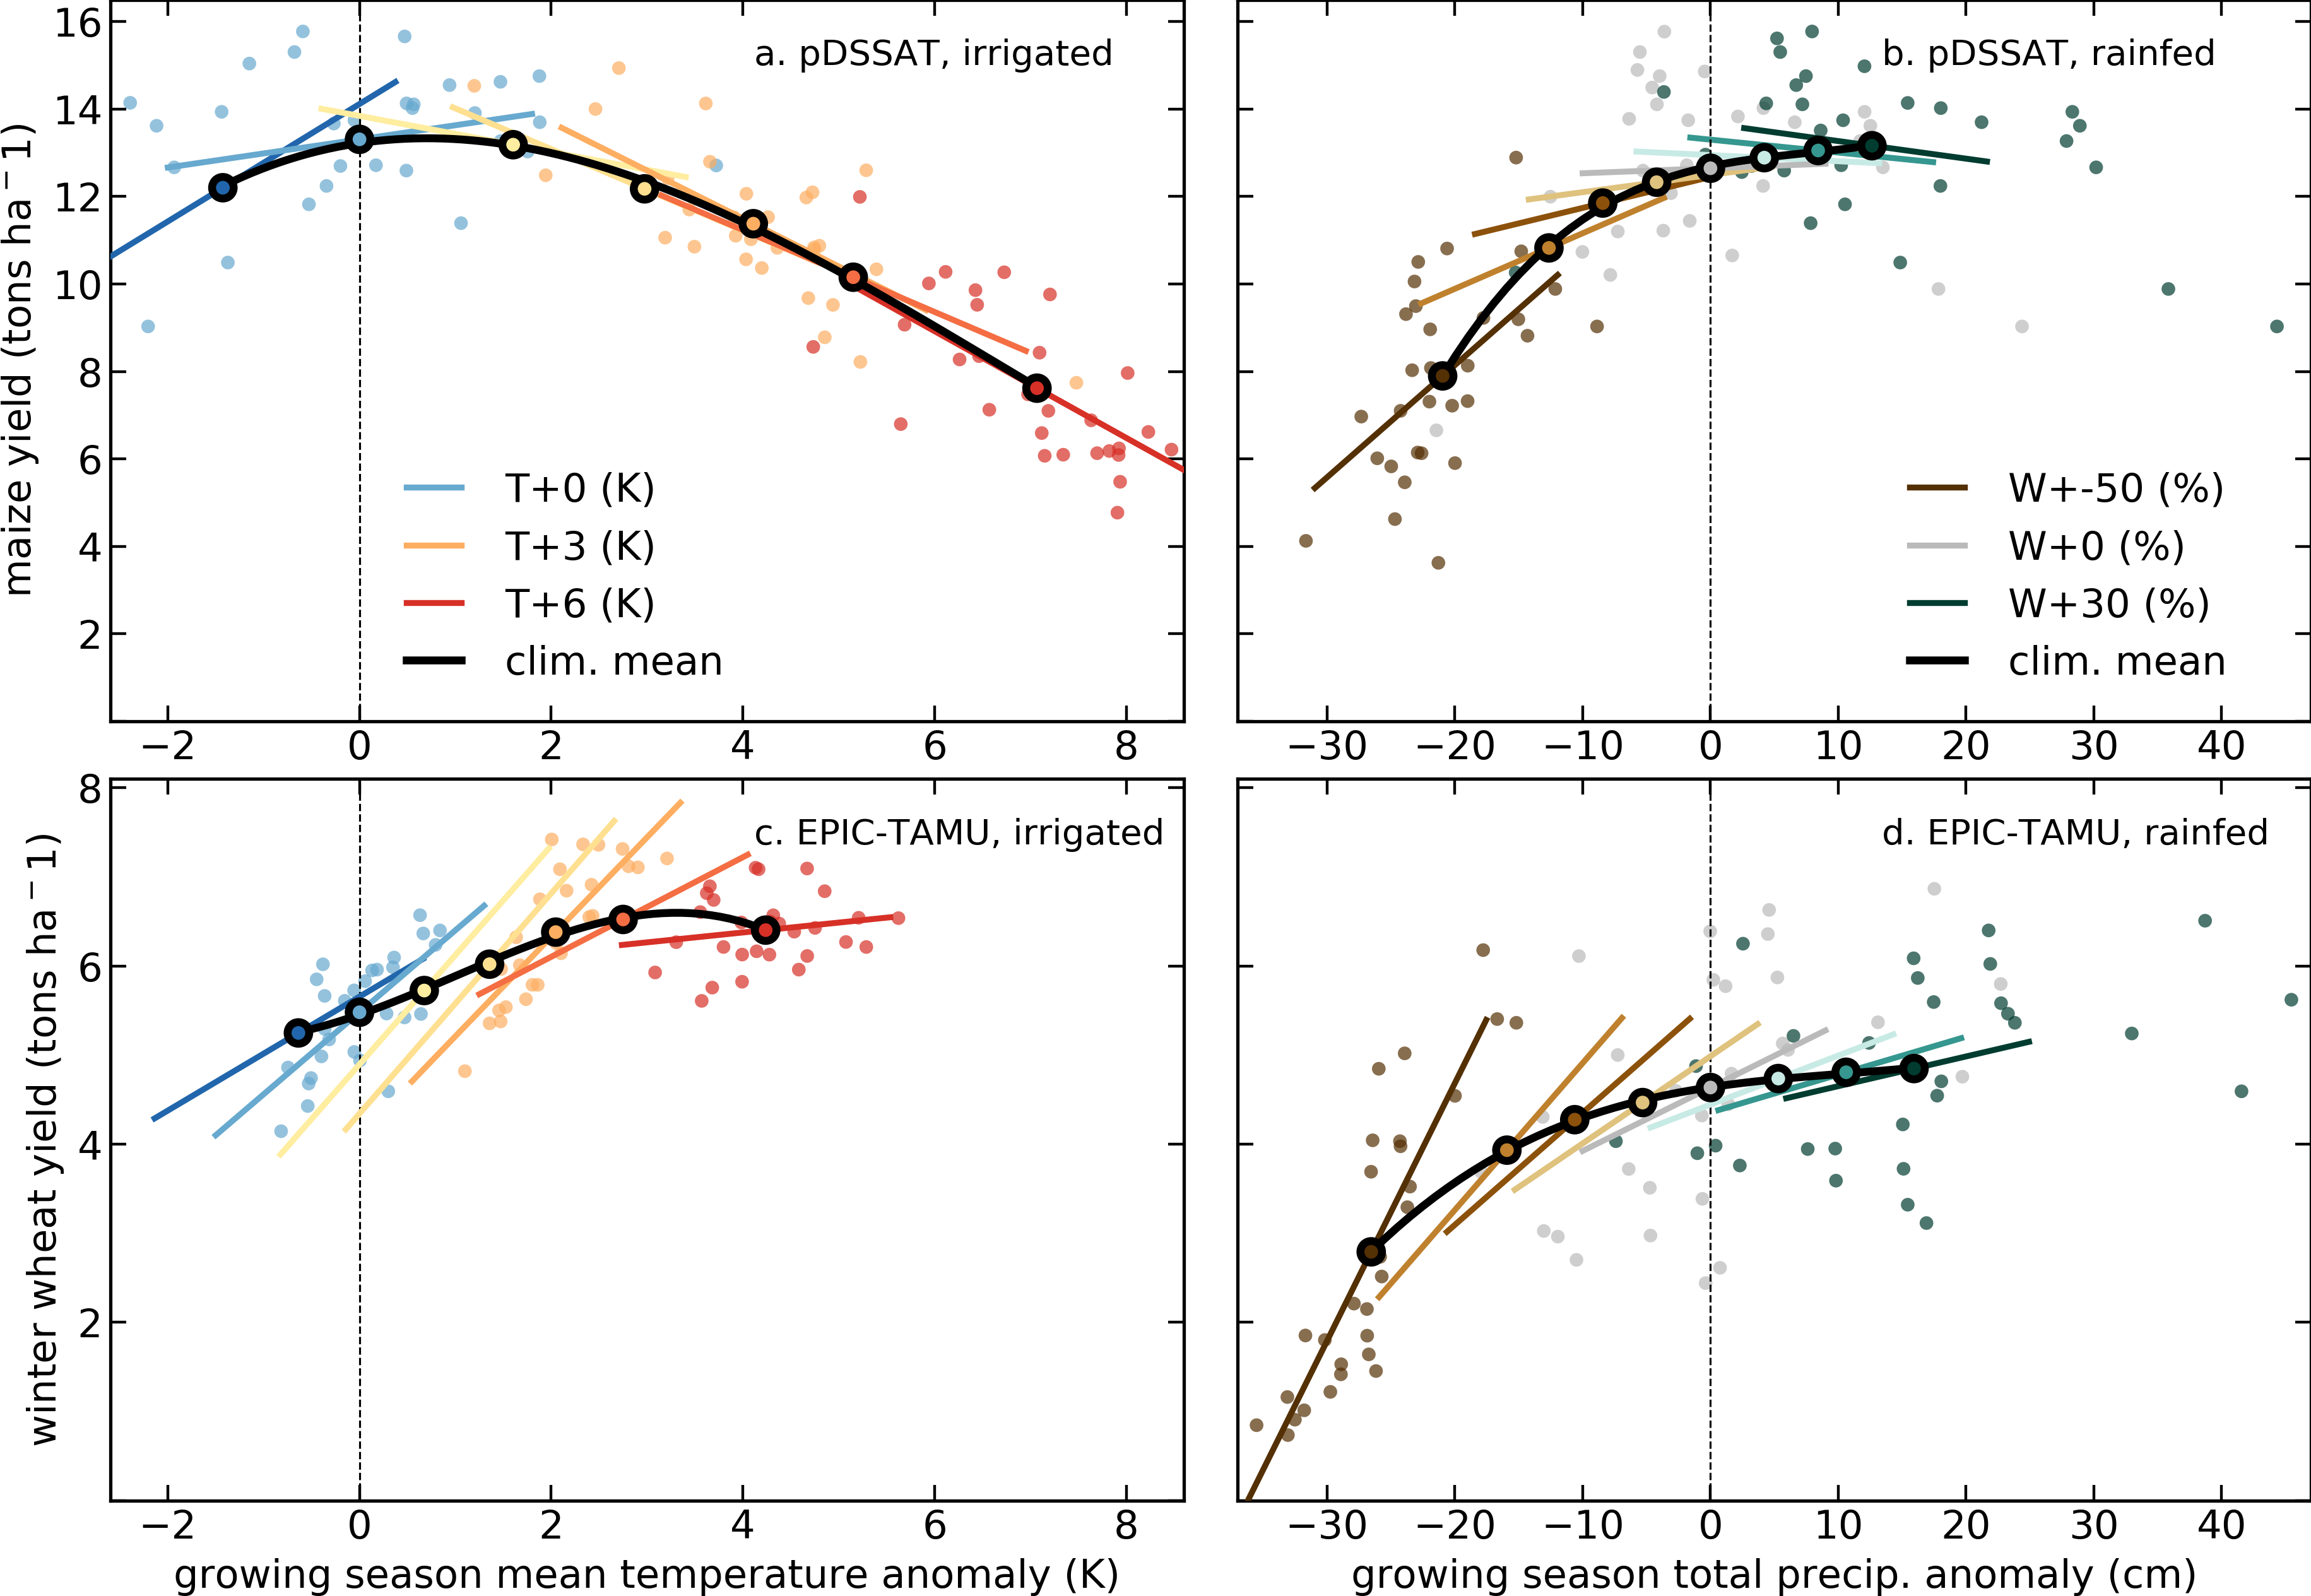
\includegraphics[width=15cm]{figures/phase_II_em_figure_1.png}
   \caption{
	   Example showing distinction between crop yield responses to year-to-year and climatological mean shifts in climate variables, for maize from the pDSSAT model in a representative high-yield region (grid cell in northern Iowa, top row) and for winter wheat in France in the EPIC-TAMU model (bottom row).
	Left column (\textbf{a \& c}) are irrigated crops, all temperature cases % (T-1, +0, +1, +2, +3, +4, +6) 
	with other variables held at baseline values, and right column (\textbf{b \& d}) are rainfed crops, all precipitation cases. %(W -50\%, -30\%, -20\%, -10\%, W, +10\%, +20\%, +30\%).
       Open black circles mark climatological mean yields and bold black lines show a 3rd order polynomial fit through them. 
       Colored lines show linear regressions (by orthogonal distance regression) through the 30 annual yields of each parameter case. 
       Colored circles show annual yields for selected cases. %.: \textbf{left}: T+0 (blue) and T+6 K (red), and \textbf{right}: W-50\% (brown) and W+30\% (green).
       Differences in slopes of colored and black lines mean that responses to year-over-year fluctuations differ from those to longer-term climate shifts. Differences are generally stronger for wheat (bottom) than maize (top).  
       Note that for rain-fed crops, slope differences in this representation could also result from correlated precipitation and temperature fluctuations in the baseline timeseries, but P-T correlations do not contribute to the effects shown here. 
       Such correlations would complicate emulations based on year-over-year yields but would not necessarily bias them.
       See Supplemental Figures S4-S8 for other crops, models, and locations.
       %For precipitation, responses to year-over-year responses resemble those to climatological shifts -- colored lines are approximately tangent to black line -- but the both responses are highly nonlinear. % Maize and soy are more regular in temperature, wheat and rice are not. Precip is irregular in ever case as far as I can tell.% For temperature, responses to year-over-year fluctuations are very different from those to longer-term climate shifts for some crops: slope of colored and black lines differ. %For precipitation, responses to year-over-year responses resemble those to climatological shifts -- colored lines are approximately the tangent of the black line -- but the climatological response is highly nonlinear.
       }
   \label{fig:yearvclim}
\end{figure*}

While differences in responses at different timescalescan arise for many reasons, including memory in the crop model or lurking covariates, the most likely explanation here is that the regressors used, mean growing-season temperature or precipitation, do not fully describe the conditions that affect crop yields. 
The mean growing-season value is only a proxy for the distribution of daily climatic conditions that crops are sensitive to, and present-day variations between years can be very different from future forced changes. 
That is, variations in growing-season \textit{means} from year to year at present are associated with changes in growing-season \textit{distributions} that are unrelated to any changes in future warmer climates: a warm year at present may be quite different from a warm year in the future \citep[e.g.][]{Ruane2016}. % XX not sure this is the right citation for this...
Changes in temperature distributions have been shown to strongly affect crop yields \citep[e.g.][]{Hansen2000, Gadgil2002}, though precipitation effects should be smaller since crops respond not to rainfall but to soil moisture, which integrates over weeks or even months \citep[e.g.][]{potter2005effects, Glotter14, CHALLINOR200499}. 

A second factor of importance is that any nonlinearity in crop responses will itself lead to a distinction between climatological and year-over-year fits, even if distributional differences are irrelevant. 
Given the interannual variations in the climate timeseries, the mean annual yield response to a perturbation is not the same as the response of the climatological mean yield. 
The effect of nonlinearity may be particularly relevant for precipitation, since model crop yields drop steeply and nonlinearly with increasing dryness. 
(Crop yields should drop under excess precipitation as well, but process-based models do not capture losses in saturated conditions well \citep[e.g.][]{Glotter15,Li2019}.) 

In the GGCMI Phase II experiment, the imposed perturbations involve no changes in underlying distributions. % (reasonable since summertime change are expected to be small \textcolor{red}{cite}).
The choice is reasonable, since climate models do not agree on distributional changes.
However, most models do project small mean increases in growing-season temperature variability for many areas, and projected changes can be substantial in more localized regions, though models disagree on spatial patterns.
For example, in business-as-usual climate projections to the year 2100, growing season temperature variability over currently cultivated rice areas in the HadCM3L model increases by 31\%, though in CESM1-0-1 model it decrease by 12\%. 
(See Supplemental Table S1 for results from multiple climate models for the different crops).
We therefore explicitly test (in Section \ref{S:4.3}) the assumption that distributional changes are not consequential for climatological mean yields, by confirming that an emulator trained on the GGCMI Phase II dataset can successfully reproduce yield changes under a full climate model projection.

\begin{figure*}[ht]
\centering
   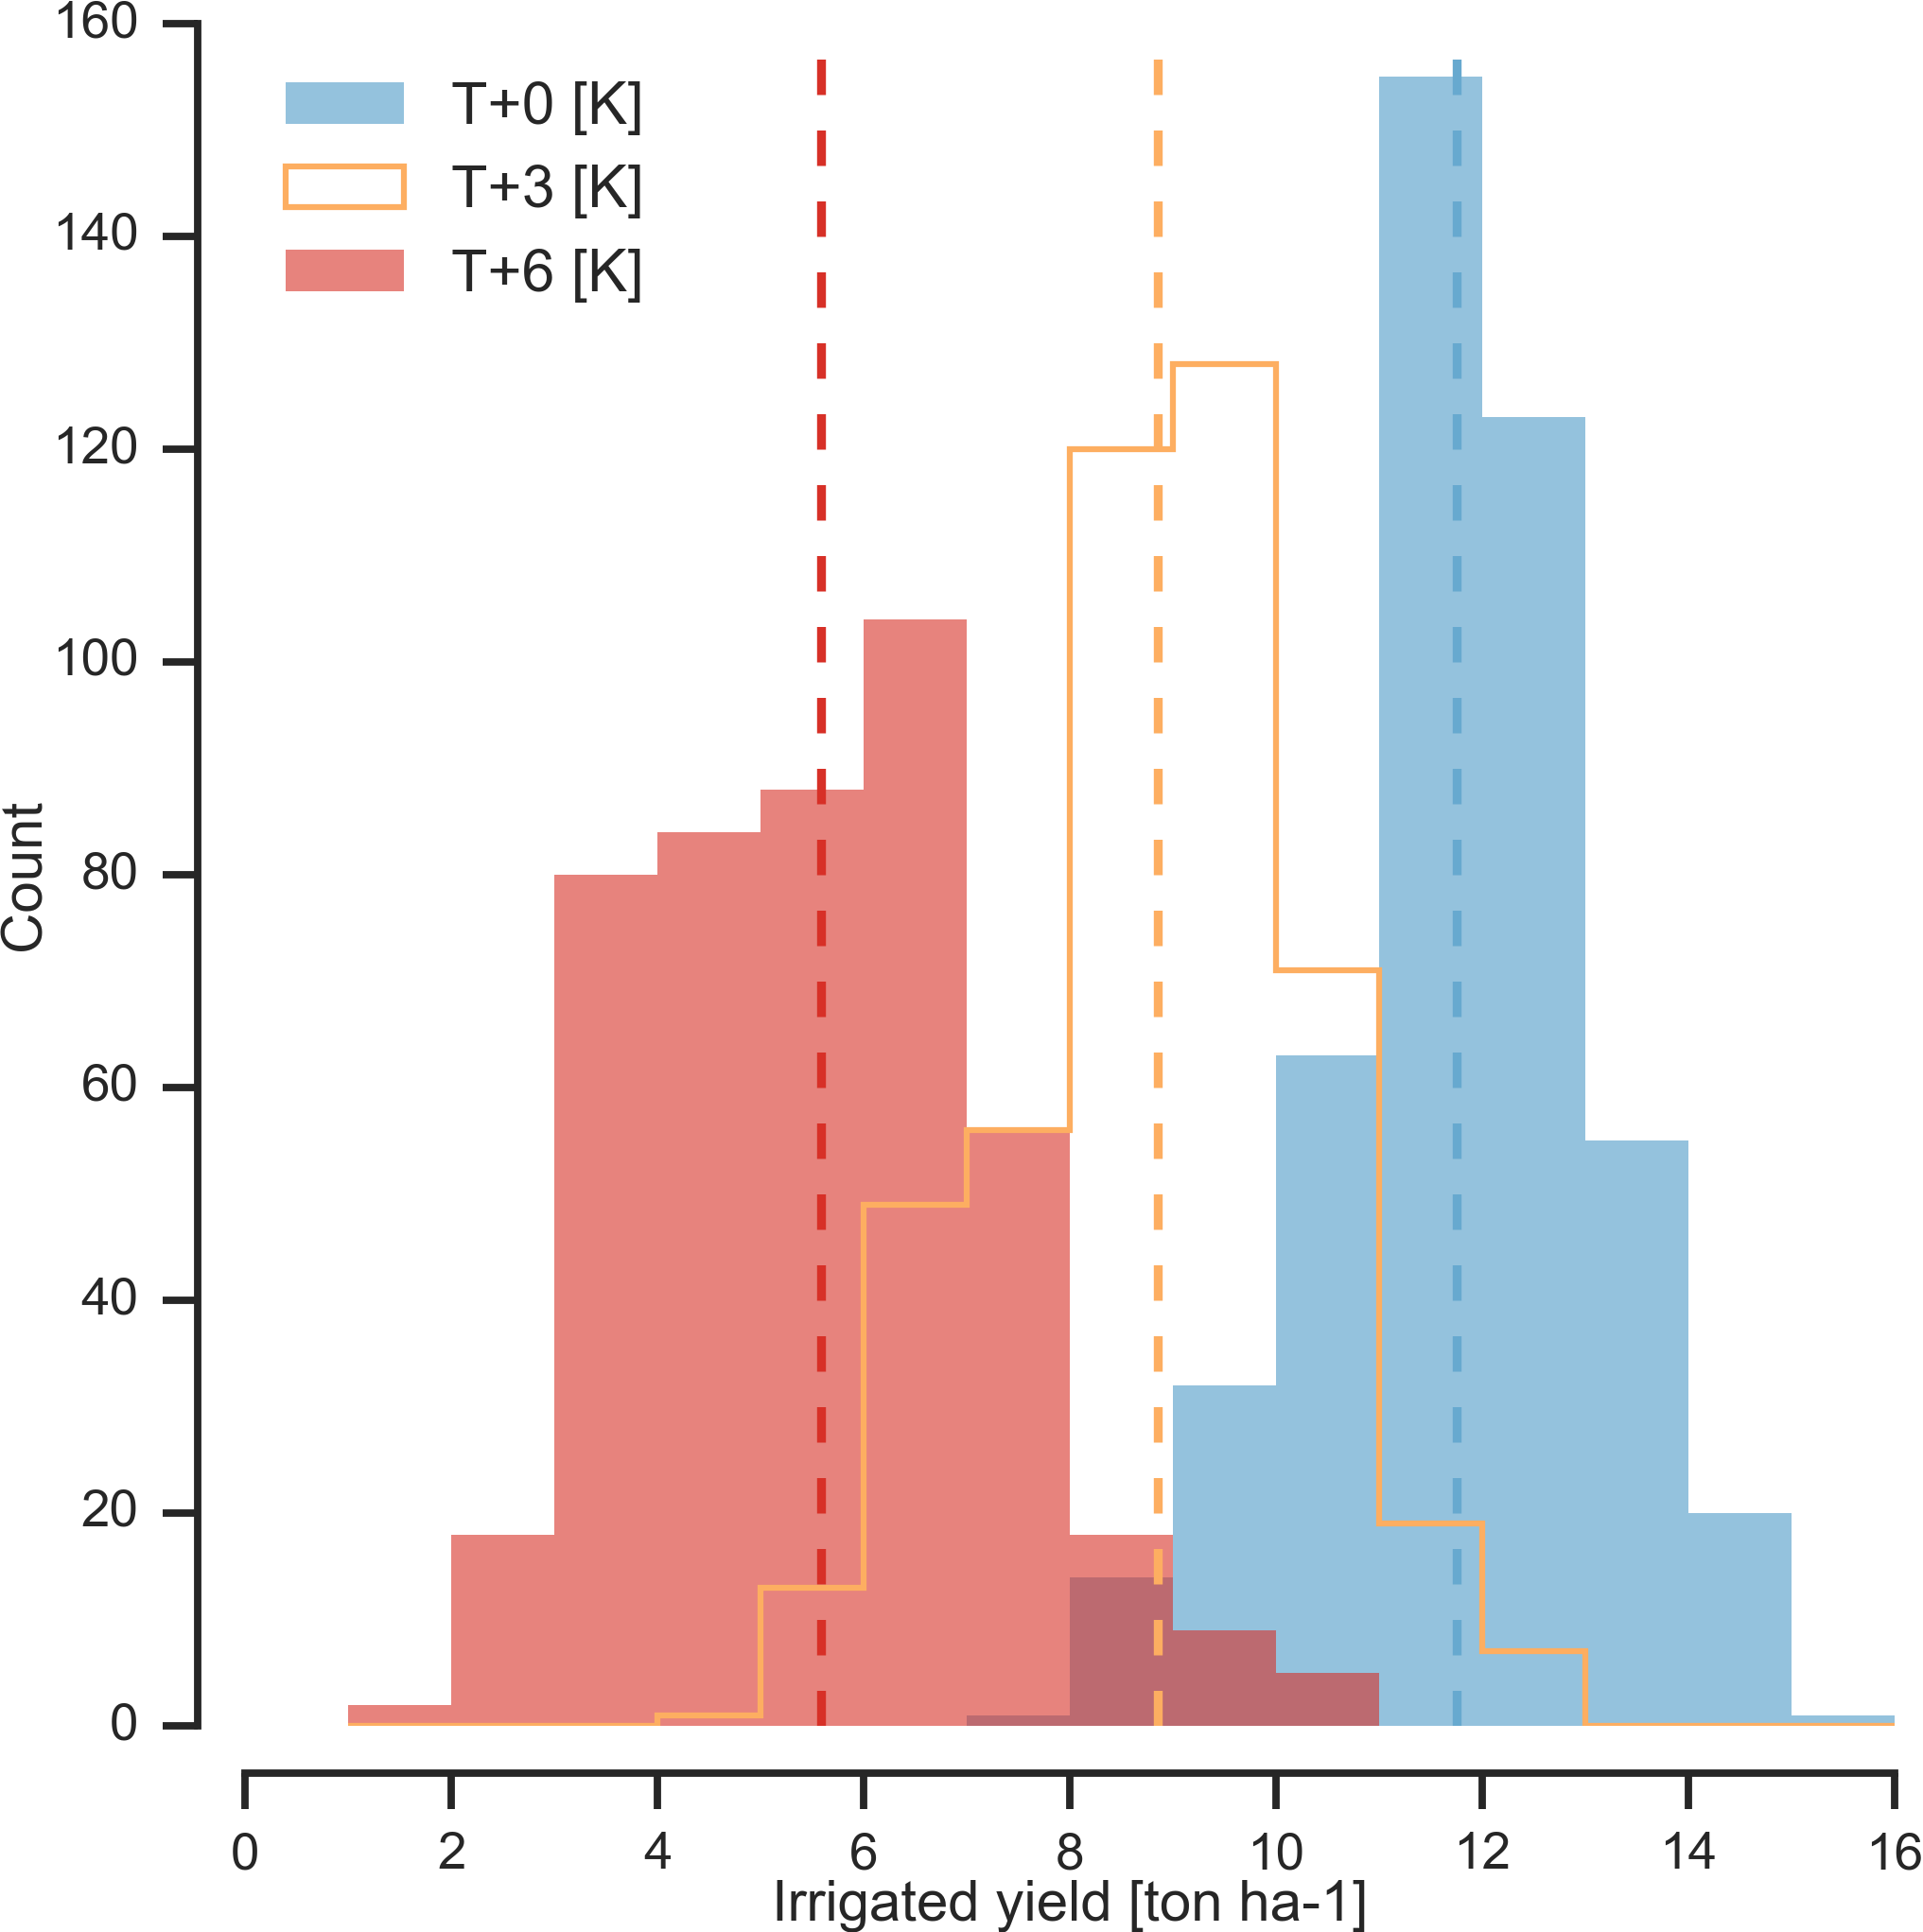
\includegraphics[width=7cm]{figures/hist_year_t.png} \hspace{10mm} 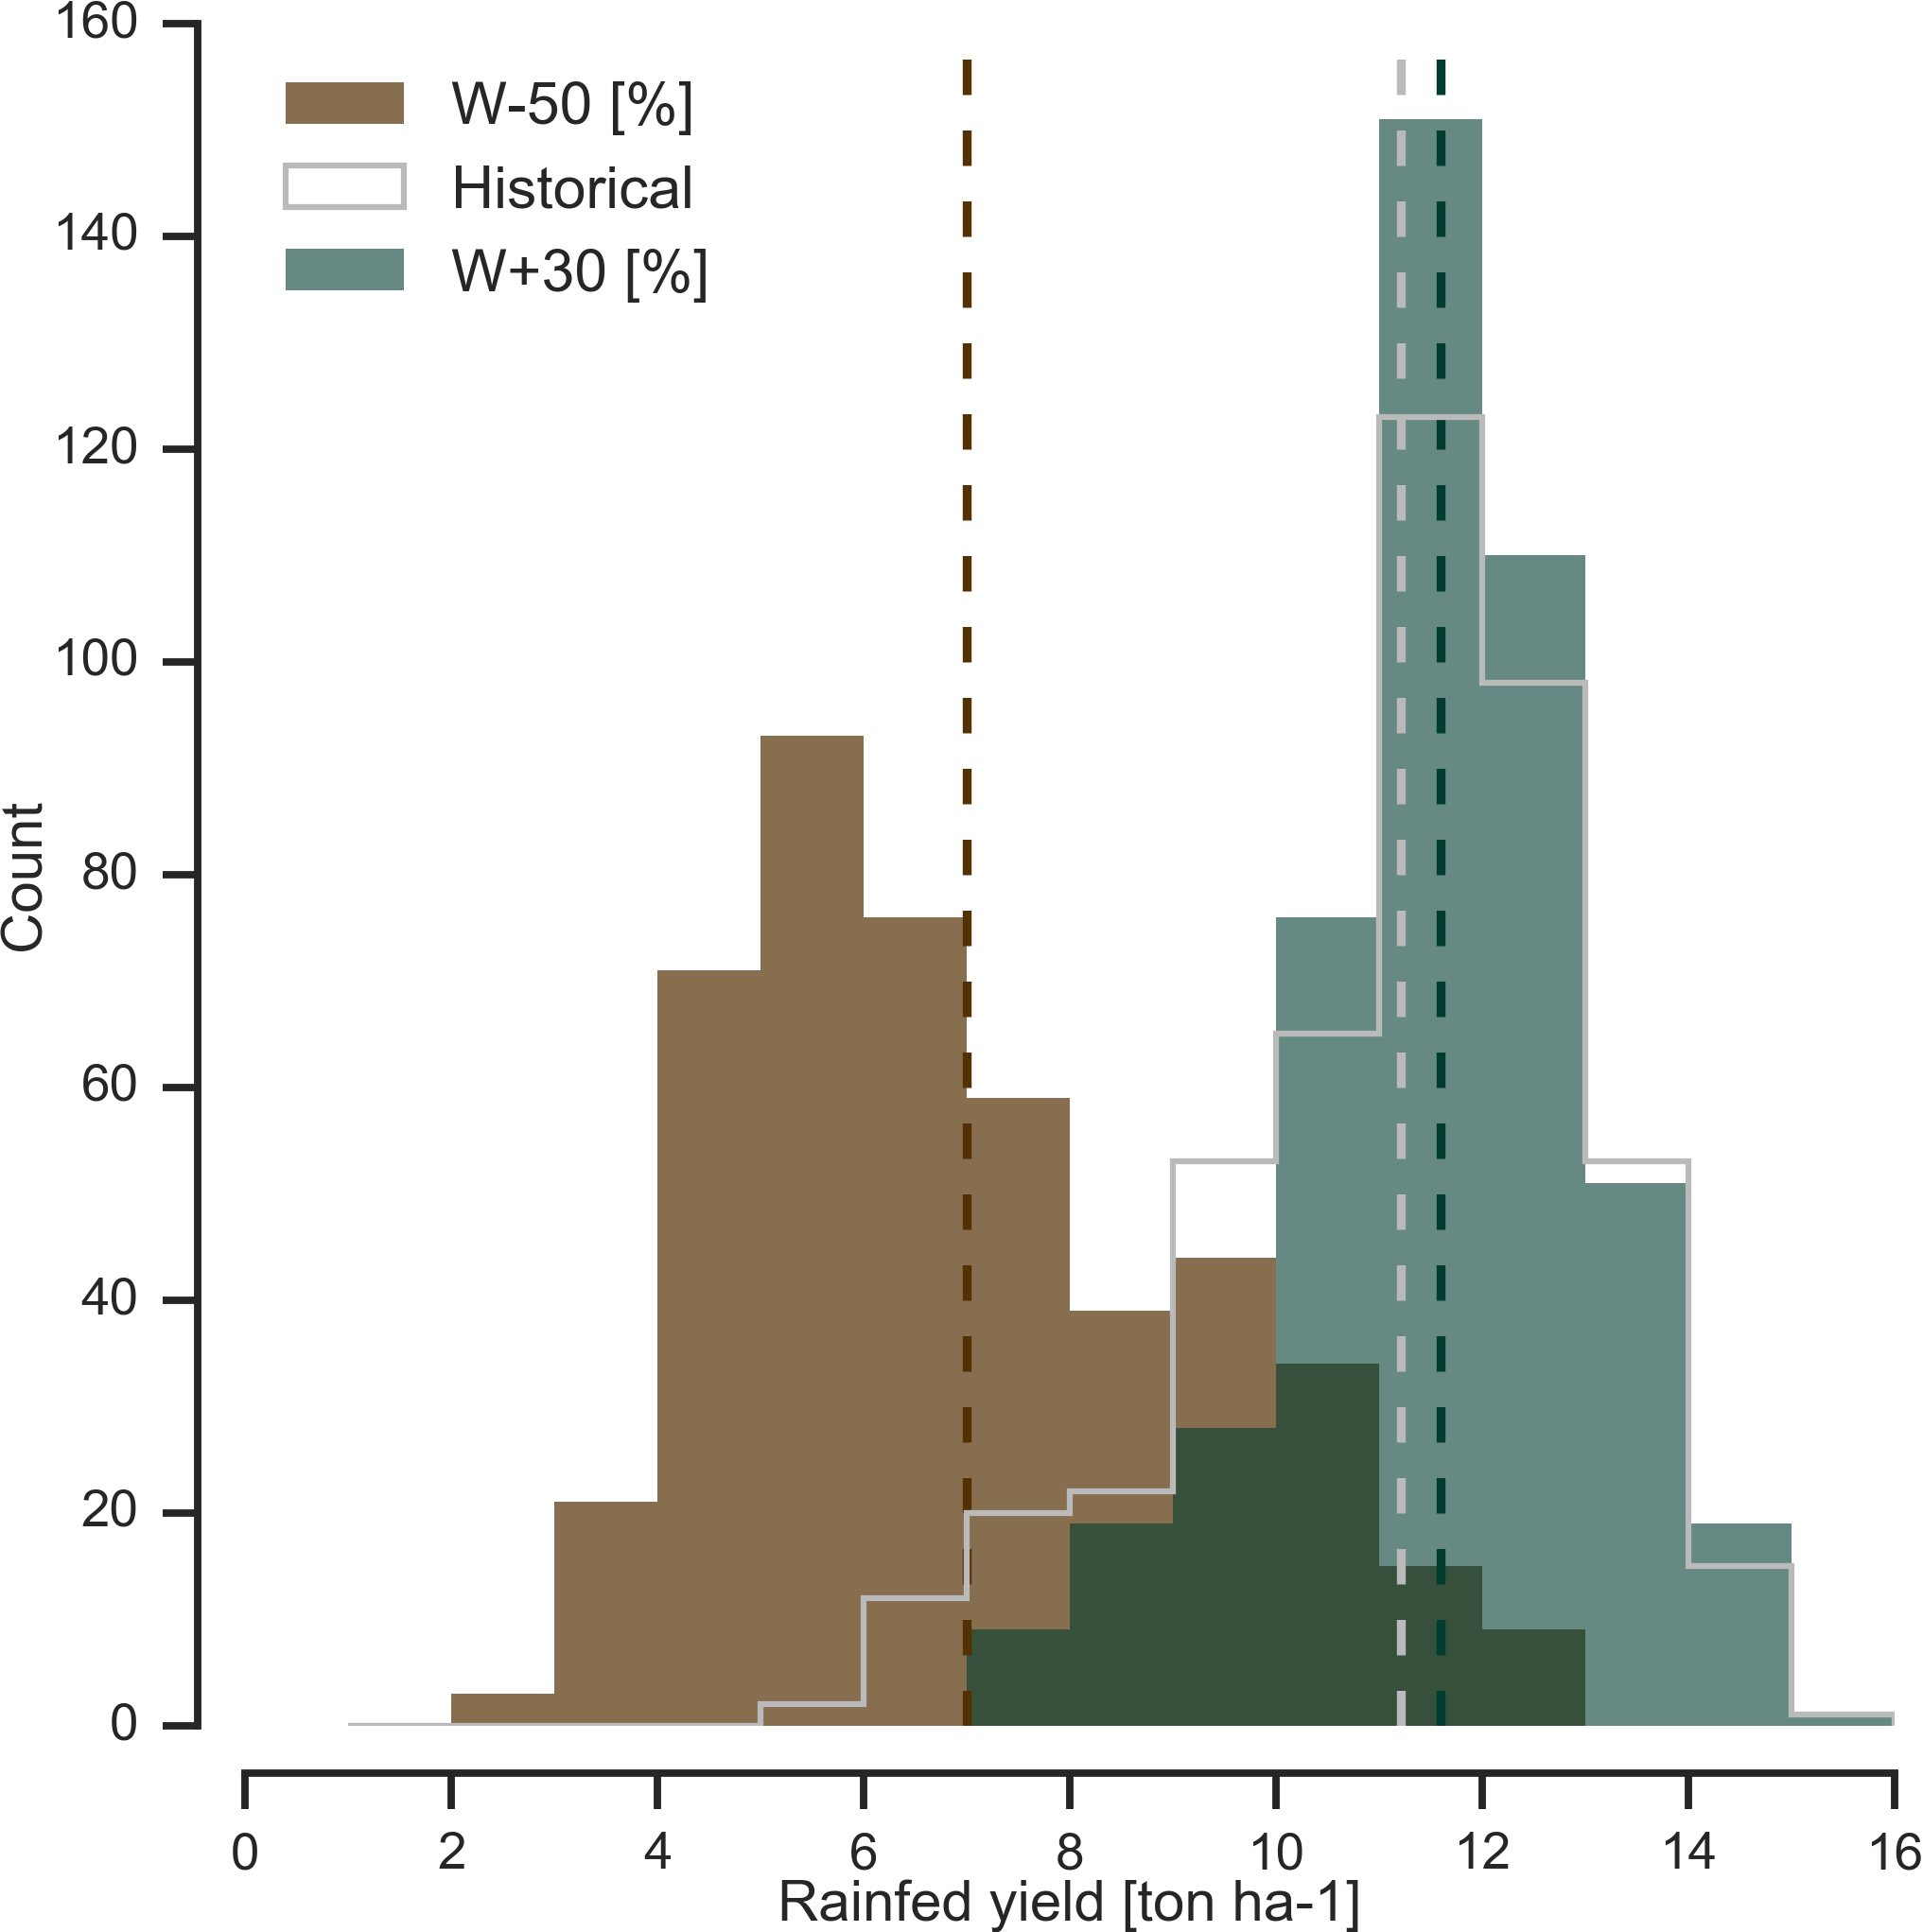
\includegraphics[width=7cm]{figures/hist_year_pr.png}
   \caption{
   Example showing results of increased crop yield sensitivity to year-over-year climate variations under climate stress. 
	Yield distributions are from examples of Figure \ref{fig:yearvclim}, top row, of maize in Iowa, (\textbf{left}) for irrigated maize in scenarios of altered temperature and (\textbf{right}) for rainfed maize in scenarios of altered precipitation.
	Because yield sensitivities rise under strong warming or drying, distributions of year-over-year crop yields widen in T+6  and P-50\% scenarios relative to present-day simulations, even though all input climate timeseries have identical variance for temperature. Note: precipitation changes have different variance since the perturbations are fractional.  
    }
   \label{fig:yearly}
\end{figure*}

Note that even though distributions of climate variables are unchanged in the GGCMI Phase II simulations, the spread in annual yields still becomes wider in highly impacted climate states, because of the nonlinearity of yield responses (Figure \ref{fig:yearly}). 
In the GGCMI Phase II dataset, all crops except rice show  greater year-to-year yield variance  in conditions of extreme climate stress. %, as crop yields become more sensitive to additional perturbations. % because yield sensitivities to perturbations increases. 
(Rice is typically irrigated and experiences no water stress.) 
This effect has been noted in previous studies. For example, \cite{Urban2012} found an increase in yfield variance of U.S.\ maize of \textcolor{red}{20\% per degree K temperature rise}, using a combination of climate model projections and statistical models trained on present-day yields. While the authors do not diagnose a specific cause of that increase, they discuss multiple potential mechanisms, including nonlinearity in responses. 


%%%%%%%%%%%%%%%%%%%%%%%%%%%%%%%%%%%%%%%%%%%%%%%%%%%%
%%%%%%%%%%%%%%%%%%%%%%%%%%%%%%%%%%%%%%%%%%%%%%%%%%%%
\section{Emulation}
\label{S:3}
Emulation involves fitting individual regression models from GGCMI Phase II output for each crop and model and 0.5 degree geographic pixel; the regressors are the applied perturbations in CO$_2$, temperature, water, and nitrogen (CTWN). 
We discuss here largely emulations of climatological mean crop yield with no growing season adaptation (A0 scenarios), but note that any output of the crop models can potentially be emulated. 
We provide separate emulations of not only irrigated and rainfed yields but also applied irrigation water (pirrww in mm\ yr$^{-1}$, see \citep{Franke2019a}) in both the A0 and A1 growing season, meaning that each model and crop combination results in six sets of regressions. (See Supplementary Material SXX for more information on additional cases not shown.)

\subsection{Statistical model and feature importance}
For the statistical model of crop yields as a function of CTWN, we choose a relatively simple parametric model with a 3rd-order polynomial basis function (Equation \ref{eqn:features_original}). 
If the climatological mean response is relatively smooth, then a simpler form provides a reasonable fit that allows for some interpretation of resultant parameter weights. 
A relativity simple parametric form also allows fast model emulation at the grid cell level as opposed to the global or large regional level. 
By emulating at the grid cell level, we indirectly include any yield response to geographically distributed factors such as soil type, insolation, and the baseline climate, and preserve the spatial resolution of the parent models.
To facilitate potential parameter-by-parameter comparison across crop models, we hold the functional form constant in space, across all crops, and models. 
That is, the same statistical model is used for all grid cells, models, and rainfed crops. 
Note however that regressions for irrigated crops do not contain W terms and models that do not sample the nitrogen levels omit the N terms.
With all higher order terms included (minus $N^{3}$), the resultant model contains 34 terms (Equation \ref{eqn:features_original}). 
We necessarily omit the N$^3$ term, which cannot be fitted because we sample only three nitrogen levels, but retain other higher-order N terms. 
Results shown for the remainder of the paper use this specificaiton.


\begin{align}
    \label{eqn:features_original}
    Y\ = \ & K_{1}  \\
    + \ & K_{2} C     + K_{3} T      + K_{4} W      + K_{5} N  + K_{6} C^2 \nonumber \\
    + \ & K_{7} T^2    + K_{8} W^2    + K_{9} N^2 + K_{10} C W \nonumber \\
    + \ & K_{11} C N   + K_{12} T W   + K_{13} T N + K_{14} W N \nonumber \\
    + \ & K_{15} C T + K_{16} T^3  + K_{17} W^3  + K_{18} C^3 + {\color{dark-gray}K_{*} N^3} \nonumber \\
    + \ & K_{19} T W N + K_{20} T^2 W + K_{21} W^2 + K_{22} W^2 N  \nonumber \\
    + \ & K_{23} C W N + K_{24} C T N + K_{25} C T W + K_{26} N^2 C \nonumber \\
    + \ & K_{27} N^2 T + K_{28} N^2 W + K_{29} T^2 N + K_{30} T^2 C  \nonumber \\
    + \ & K_{31} W^2 C + K_{32} C^2 W + K_{33} C^2 T + K_{34} C^2 N \nonumber
\end{align}

Both higher-order and interaction terms are expected to be important for representing crop yields. Higher order terms are needed because crop yield responses to weather are well-documented to be nonlinear: e.g.\ \citet{Schlenker2009} for T perturbations and \citet{He2016} for W (precipitation). 
Interaction terms are needed since the yield response is expected to depend on interactions between the major inputs. 
For example, \citet{Lobell2007} and \citet{Tebaldi2008} showed that in real-world yields (with C and N fixed), the joint distribution in T and W is needed to explain observed yield variance.  
Other observation-based studies have shown the importance of the interaction between W and N \citep[e.g.][]{AULAKH2005}, and between N and C \citep{Mitsuru92, Nakamura97}.

We do not focus in this study on comparing different functional forms or non-parametric models and instead focus on feature importance.
Some prior studies have used other statistical specifications in crop model emulation: for example, \citet{BLANC2015} and \citet{BLANC2017} use a 39 term fractional polynomial. 
Such a high-dimensional model is difficult to fit, especially for a training set of realistic simulations in which input parameters are highly correlated, and  \citet{BLANC2015} and \citet{BLANC2017}  ``borrow information across space'' by fitting grid points simultaneously across soil region in a panel regression. 
Our simpler functional form can be fit independently at each grid cell while still providing a satisfactory emulation of all GGCMI crop models and crops. 
(See Section \ref{S:4} for evaluation of emulator fidelity.)

To investigate the relative importantce of terms in the statical model and to improve the interpretability of the terms, we apply a feature selection cross-validation process in which terms in the polynomial are tested for importance.
In this procedure higher-order and interaction terms are added successively to the regression model one by one, and we calculate an aggregate mean absolute error with each increasing terms and eliminate those terms that do not contribute significant reductions in error (top row of Figure \ref{fig:features}). 
Some terms that did not reduce the aggregate error are included if a higher order version of that term provided a decrease in mean squared error: for example, the $T^3$ term cannot be included without also taking the $T^2$ and $T$ terms. 
We select terms by applying the feature selection process to three example models: two that provided the complete set of 672 rainfed simulations (pDSSAT, EPIC-TAMU, and one that provided the smallest training set (121 input combinations, PEPIC). 
Feature importance is not uniform due to spatial heterogeneity across models and crops, so we weight the loss function by currently cultivated area during this step. 
The resulting choice of terms is then applied for all emulators and all crops. 
Since the goal of the emulator is interpolation within the sample space and not extrapolation, we err on the side of including terms that are useful in at least some cases, because the added predictive ability outweighs the costs to distribution of the residuals or over-fitting.  

\begin{figure*}[ht]
\centering
   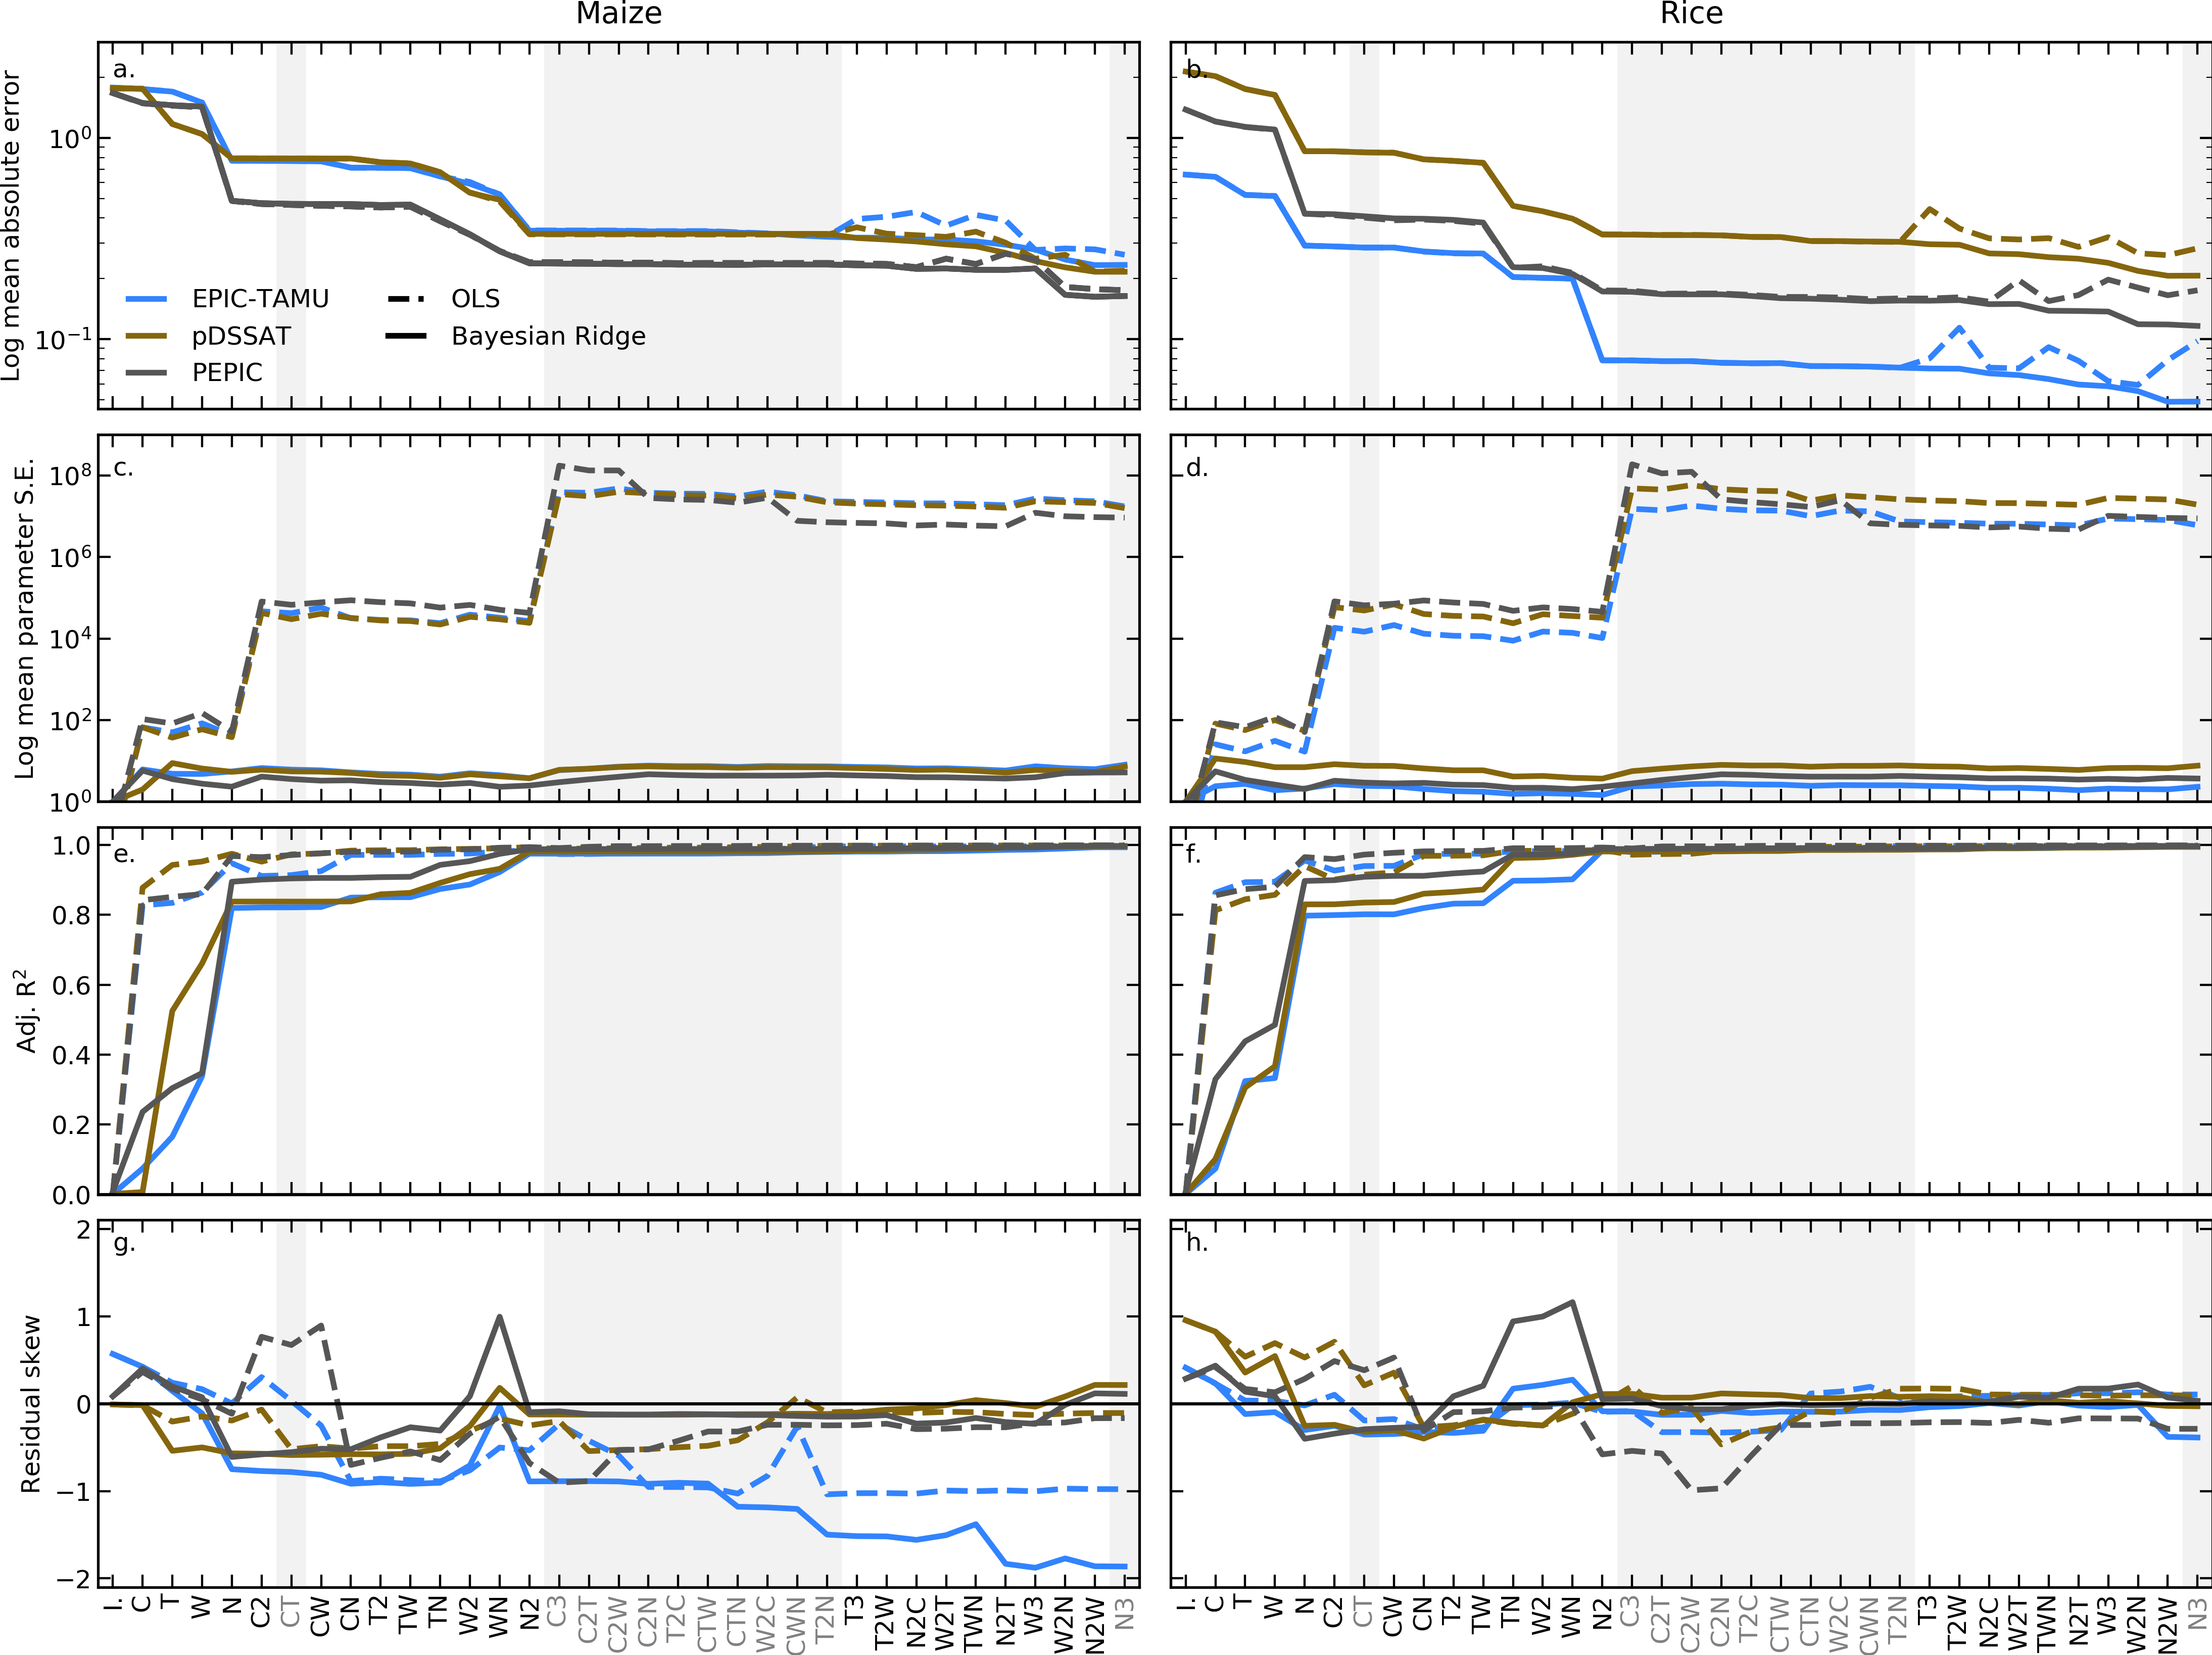
\includegraphics[width=16.3cm]{figures/model_select_maize_rice.png}
	\caption{
    Illustration of results from the polynomial feature selection process for three different crop models (colors), for all grid cells with more than 1000 ha cultivated for maize (\textbf{left}) and rice (\textbf{right}). 
    Solid lines are Bayesian Ridge regression results and dashed lines those for standard OLS. Rows show four metrics of fit quality and x axes the terms successively tested in the statistical model, sequentially added to the model in order from left to right.
    Terms that do not reduce the aggregate error are marked in {\color{dark-gray} gray} and are not included in the final model. 
    \textbf{a \& b:} log mean absolute error between emulated yield and simulated values calculated with a three fold cross validation process, where the emulator is trained on two thirds of the data and predicts the remaining third.
    \textbf{c \& d:} log mean standard parameter error. The Bayesian Ridge method strongly reduces parameter error and results in more stable estimates. 
    \textbf{e \& f:} adjusted R$^2$ score for the fit at each model specification. 
	\textbf{g \& h:} distribution of the residuals. Skewness is low at the high model specifications tested in all model cases other than EPIC-TAMU maize.
	}
   \label{fig:features}
\end{figure*}

\begin{align}
    \label{eqn:features_original}
    Y\ = \ & K_{1}  \\
    + \ & K_{2} C     + K_{3} T      + K_{4} W      + K_{5} N  + K_{6} C^2 \nonumber \\
    + \ & K_{7} T^2    + K_{8} W^2    + K_{9} N^2 + K_{10} C W \nonumber \\
    + \ & K_{11} C N   + K_{12} T W   + K_{13} T N + K_{14} W N \nonumber \\
    + \ & {\color{dark-gray}K_{a} C T} + K_{15} T^3  + K_{16} W^3  + {\color{dark-gray}K_{b} C^3} + {\color{dark-gray}K_{c} N^3}\nonumber \\
    + \ & K_{17} T W N + K_{18} T^2 W + K_{19} W^2 + K_{20} W^2 N  \nonumber \\
    + \ & {\color{dark-gray}K_{d} C W N} + {\color{dark-gray}K_{e} C T N} + {\color{dark-gray}K_{f} C T W} + K_{21} N^2 C \nonumber \\
    + \ & K_{22} N^2 T + K_{23} N^2 W + {\color{dark-gray}K_{g} T^2 N} + {\color{dark-gray}K_{h} T^2 C}  \nonumber \\
    + \ & {\color{dark-gray}K_{i} W^2 C} + {\color{dark-gray}K_{j} C^2 W} + {\color{dark-gray}K_{k} C^2 T} + {\color{dark-gray}K_{l} C^2 N} \nonumber
\end{align}

Feature importance is remarkably consistent across models (Figure \ref{fig:features}) with some notable exceptions. (JULES and PROMET for example show significant reductions in error for some of the higher order carbon interaction terms).
Even though the models exhibit different absolute levels of error, all three models agree remarkably well on feature importance, that is on  which terms reduce error and which provide no predictive benefit. (Agreement means that line slopes match in Figure \ref{fig:features}.) 
The feature selection process allows us to eliminate 12 terms, leaving a final polynomial in 23 terms.
The eliminated terms include many of those in C: the cubic; the CT, CTN, CTW, and CWN interaction terms; and all higher order interaction terms in C. 
Finally, we eliminate one 2nd-order interaction term in W and two in T. 
Implications of this choice include that nitrogen interactions are complex and important, and that water interaction effects are more nonlinear than those in temperature.  
The reduced-form emulator is acceptable across currently cultivated land for all but the JULES and PROMET models. See supplemental for addiontial information. 

\subsection{Model fitting}
To fit the parameters $K$, we use a Bayesian Ridge regularization method \citep{MacKay91} rather than standard ordinary least squares (OLS). 
The Bayesian Ridge method reduces volatility in parameter estimates when the sampling is sparse, by weighting parameter estimates towards zero, allowing the use of a consistent functional form across all models and locations. 
The choice slightly reduces mean absolute error for some of the high-order interaction terms in the model (Figure \ref{fig:features}, top row) but drastically reduces standard parameter error in the model by stabilizing the estimates (Figure \ref{fig:features}, third row).
The estimation method scores relatively lower on adjusted $R^2$ for the simplest parameter specifications, but reaches parity with the OLS at the number of terms included in this study. We use adjusted $R^2$ as a metric because additional terms are penalized (Equation \ref{eqn:rsquare}, where $n$ is the number of samples and $k$ is the number of features): 
\begin{equation}
	\centering
    \label{eqn:rsquare}
    R^{2}_{adj} = 1 - \frac{(n-1) \cdot (1 - R^{2})}{n - k}
\end{equation}
We use the implementation of the Bayesian Ridge estimator from the scikit-learn package in Python \citep{scikit-learn}. 

An additional diagnostic of a fit is the distribution of residuals. Normally or near-normally distributed residuals indicate that errors around the fit are random and not biased in some way. 
When fitting Equation \ref{eqn:features_original} to the GGCMI Phase II dataset, the distribution of the residuals depends on the number of features included in the regression, the method for estimating the parameters, and the target distribution in the training set. The residuals are only normally distributed (pvalue > 0.05 in the Shapiro–Wilk test) for a single model, PEPIC, for any specification tested here, but %  \citep{Shapiro1965}  
their skew is relatively small except in a single case, the EPIC-TAMU model for maize (Figure \ref{fig:features}, fourth row).
While including higher order terms in the model tends to reduce residual skew, the opposite occurs with EPIC-TAMU maize. 
Higher-order terms for EPIC-TAMU maize increase skew instead, but also reduce error in cross-validation, which is more important in the context of emulation.
This indicates new predictions from the emulator for EPIC-TAMU will be biased high, but with a low magnitude deviation.  

%%%%%%%%%%%%%%%%%%%%%%%%%%%%%%%%%%%%%%%%%%%%%%%%%%%%%%%%%%%%%%%
%%%%%%%%%%%%%%%%%%%%%%%%%%%%%%%%%%%%%%%%%%%%%%%%%%%%%%%%%%%%%%%
\section{Emulator evaluation}
\label{S:4}
In this section we show illustrations of the GCCMI models yield responses to climate perturbations, and evaluate metrics of emulator performance. 
Model emulation with the parametric method used here requires that crop yield responses be sufficiently smooth and continuous to allow fitting with a relatively simple functional form; we demonstrate that this condition largely holds in the GGCMI Phase II simulations. Emulation errors -- discrepancies between emulation and simulation --  are generally small, especially when compared to the differences across crop models or climate model inputs.
Emulation errors become problematic only in certain cases: in models that provide limited sampling of the GGCMI parameter space, and in some geographic locations where crops are currently not grown. 

\subsection{Yield response}
Crop yields show strong spatial differentiation across geographic regions, and emulators are able to readily reproduce these. Figure \ref{fig:map_pattern} illustrates the spatial yield pattern under current climate for one crop and model (maize in LPJmL). Absolute emulation errors are low --  99.8\% of grid cells have errors below 0.5 tons ha$^{-1}$ -- but 
emulation errors as a percentage of baseline yield can be large in areas with low potential yield and no current cultivation in the real world (e.g.\ the Sahara, Patagonia).
These regions are not currently viable for agriculture and may never become viable even under extreme climate change.  
Emulation spatial skill varies across models and crops, with maize being the quantitatively easiest to emulate across all models and locations.

\begin{figure*}[ht]
\centering
    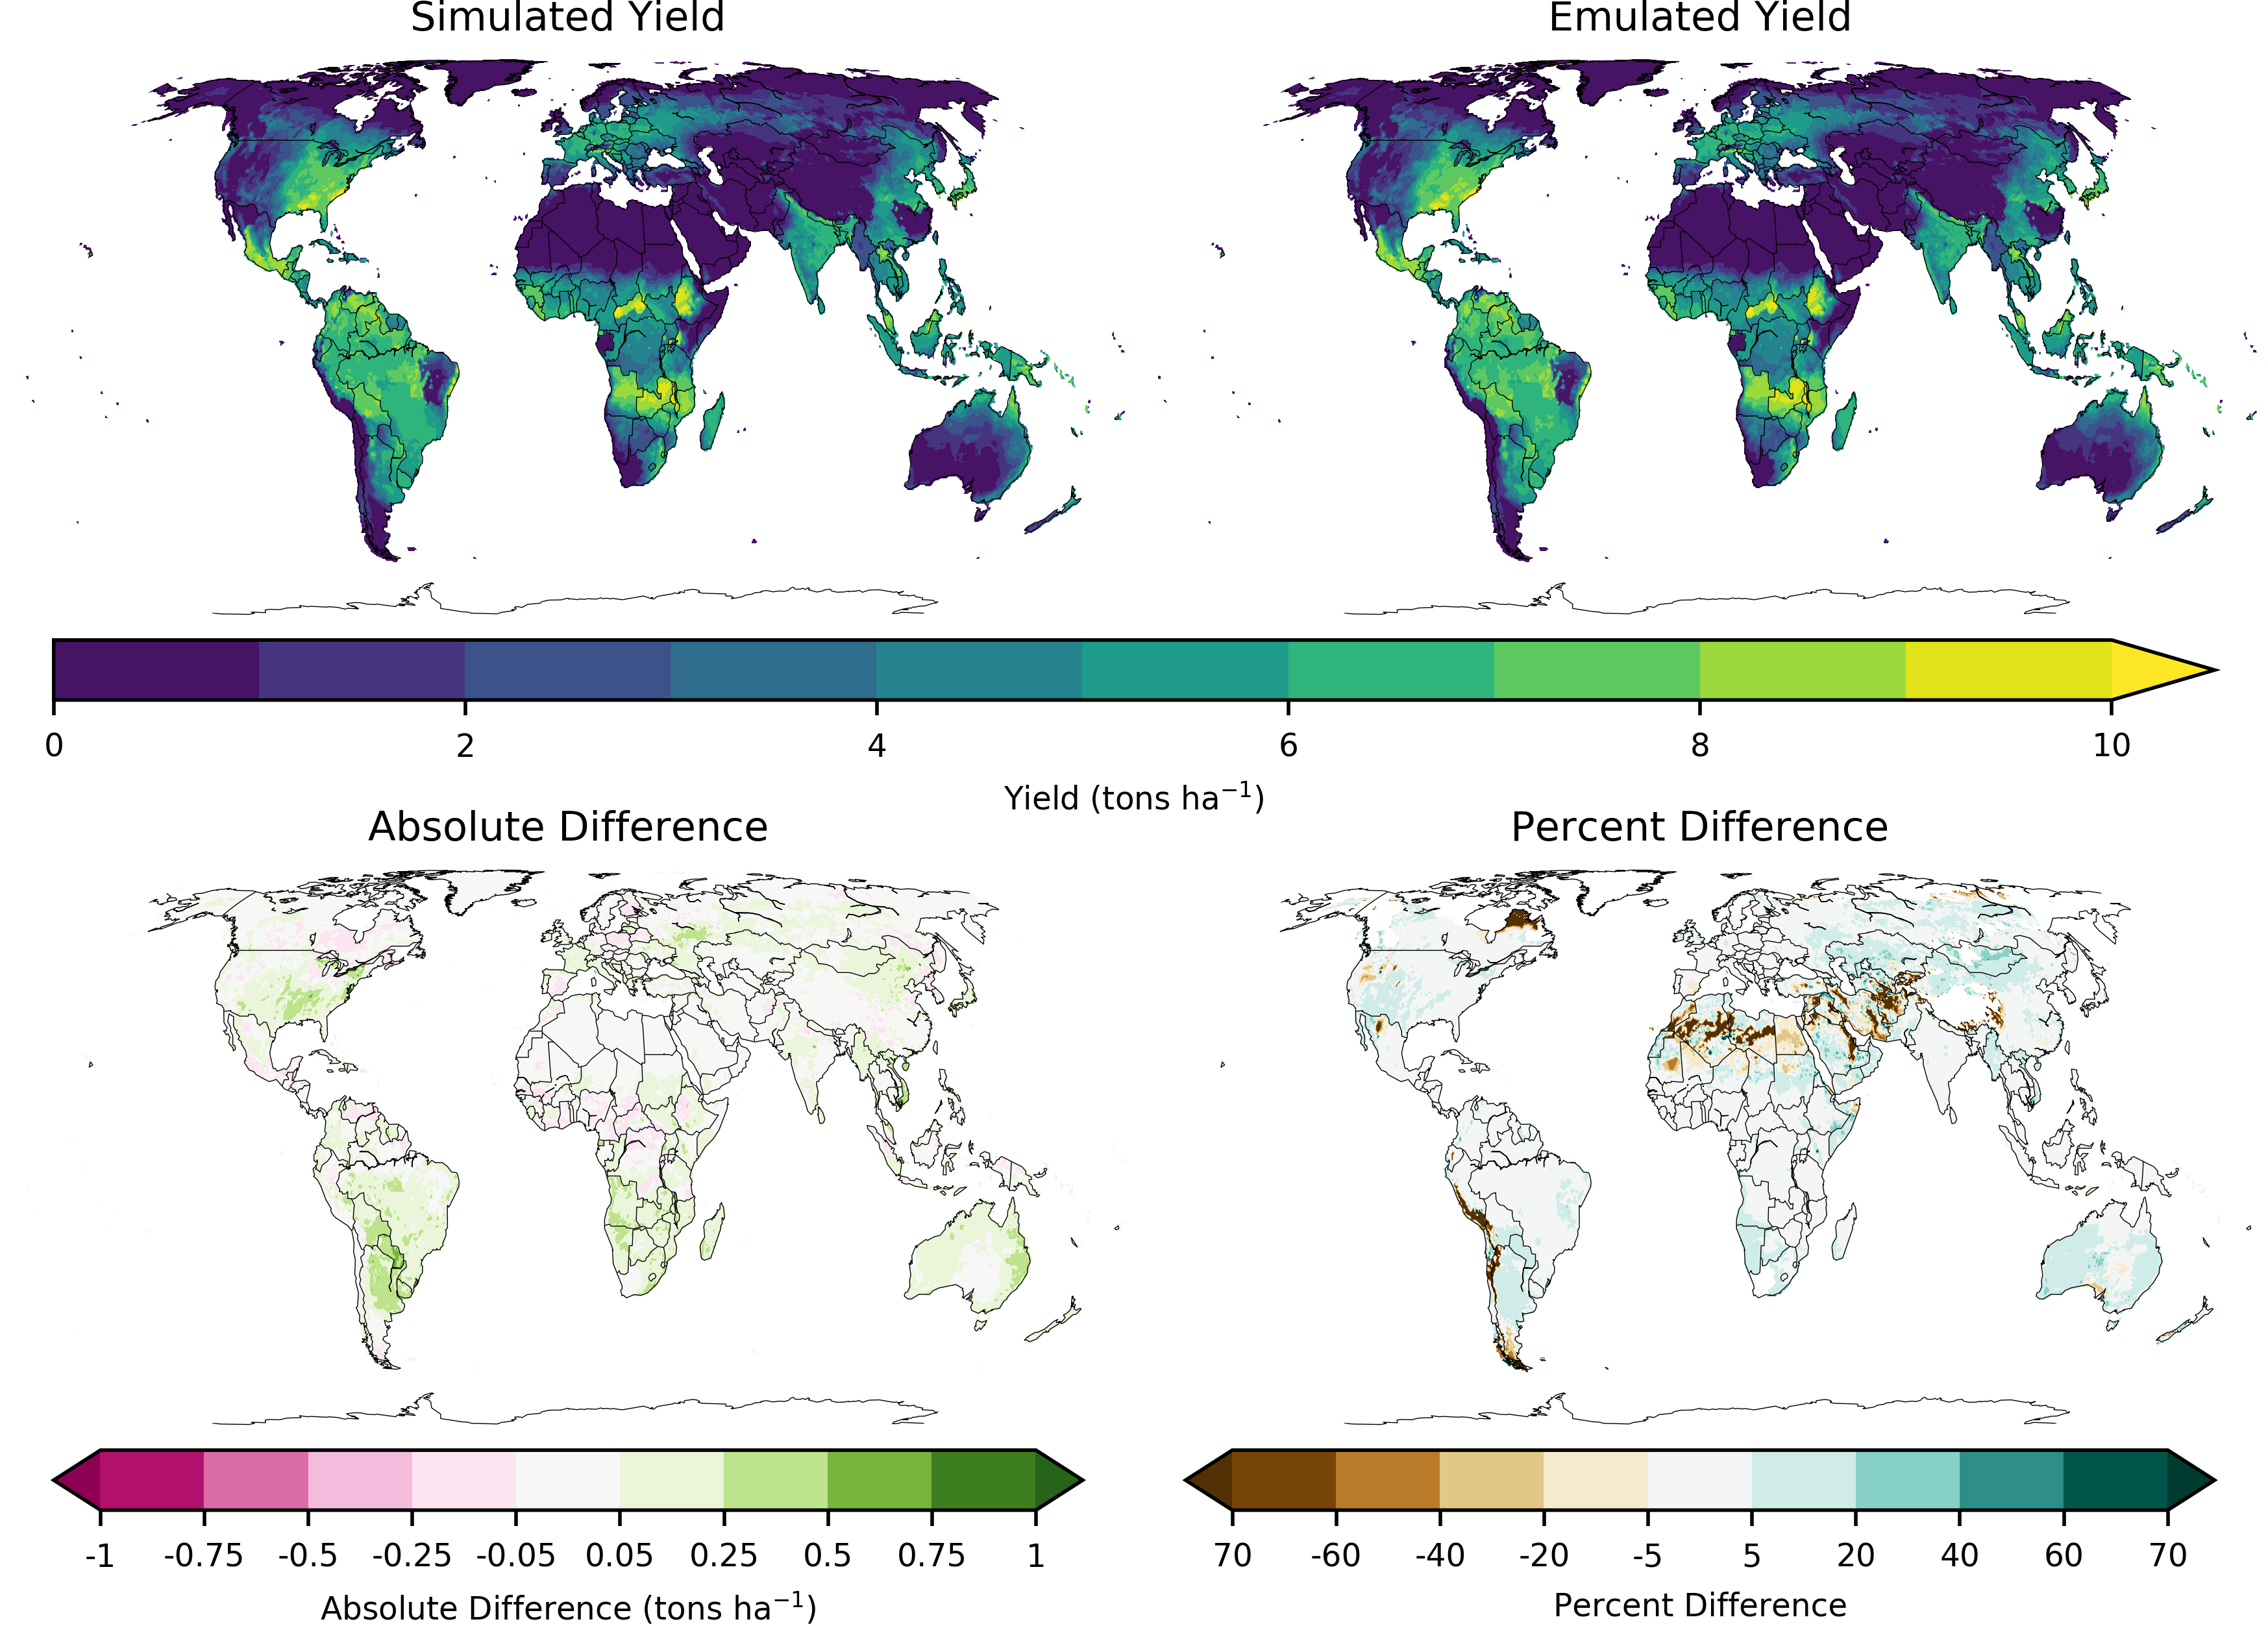
\includegraphics[width=16.0cm]{figures/lpjml_maize.png}
    \caption{
    Illustration of spatial pattern in baseline yield successfully captured by the emulator.
    Simulated (\textbf{a.}) and emulated (\textbf{b.}) yield under historical (1981-2010) conditions for rainfed maize from the LPJmL model.
    Absolute yield differences (\textbf{c.}) are less that 0.5 ton ha$^{-1}$ in almost all (99.8\%) grid cells across the globe.
    Percent difference (from simulated baseline, \textbf{d.}) is below 5\% in most (75\%) grid cells currently cultivated in the real world.
    Approximately 7\% of grid cells have errors over 20\% different from baseline, but only 3\% of grid cells with current cultivation have errors over 20\%.
    Notable exceptions include areas with very low baseline yield in the simulations including, for example, the Sahara, the Andes, and northern Quebec. 
    Percent error weighted by cultivation area globally is essentially zero (see also Table \ref{table:ASE}).
    Performance varies by crop and model. 
    See Supplementary Figure SX for more examples.
    }
   \label{fig:map_pattern}
\end{figure*}

\begin{figure*}[ht]
\centering
    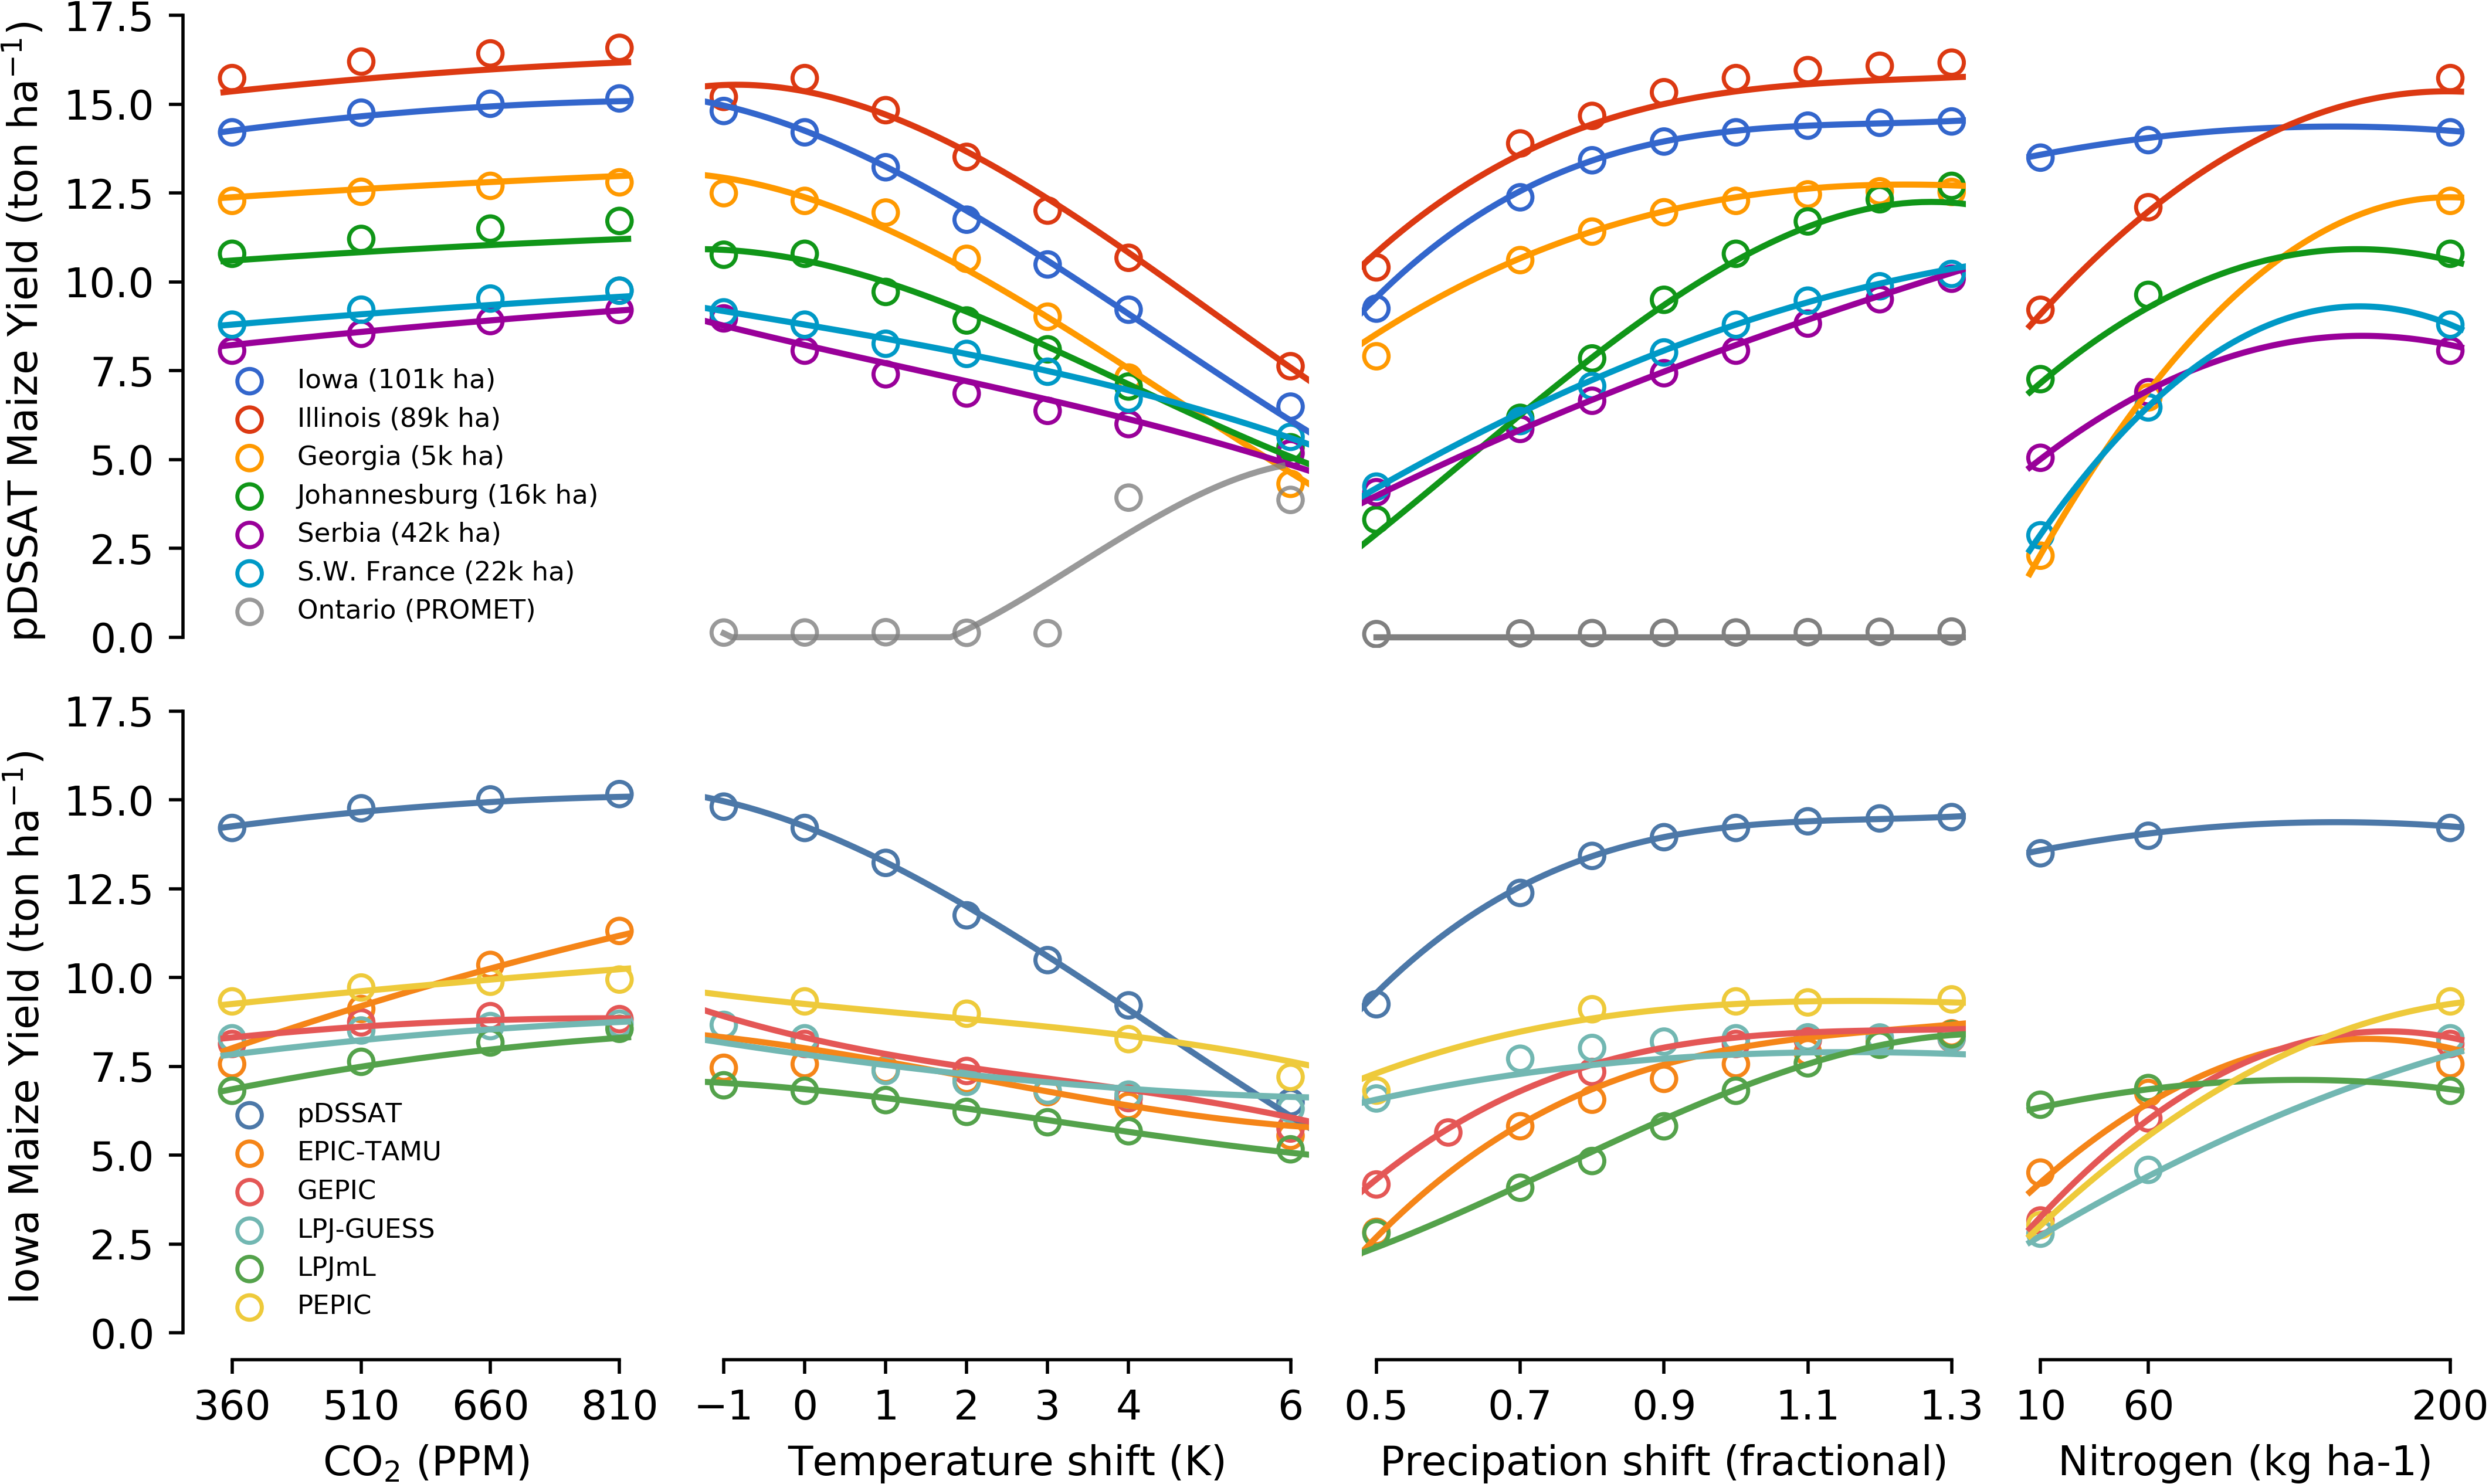
\includegraphics[width=16.3cm]{figures/regression_example.png}
    \caption{
    Illustration of spatial variations in yield response, which are successfully captured by the emulator. 
    Panels show simulations (points) and emulations (lines) of rainfed maize in the pDSSAT model in six example locations selected to represent high-cultivation areas around the globe. 
    Legend includes hectares cultivated in each selected grid cell. 
    Each panel shows variation along a single variable, with others held at baseline values. 
    Dots show climatological mean yields and lines the results of the full 4D emulator of Equation \ref{eqn:features_original}. 
    In general the climatological response surface is sufficiently smooth that it can be represented within the sampled variable space by the simple polynomial used in this work. 
    In some cases extrapolation would produce misleading results, and the emulator fails in conditions where yield response changes abruptly. 
    Failure is illustrated here by rainfed maize in north-central Ontario for the PROMET model (in gray), which shows present-day yields of zero rising abruptly if temperature warms by 4 degrees.
    }
   \label{fig:regression}
\end{figure*}

\begin{figure*}[h!!]
\centering
    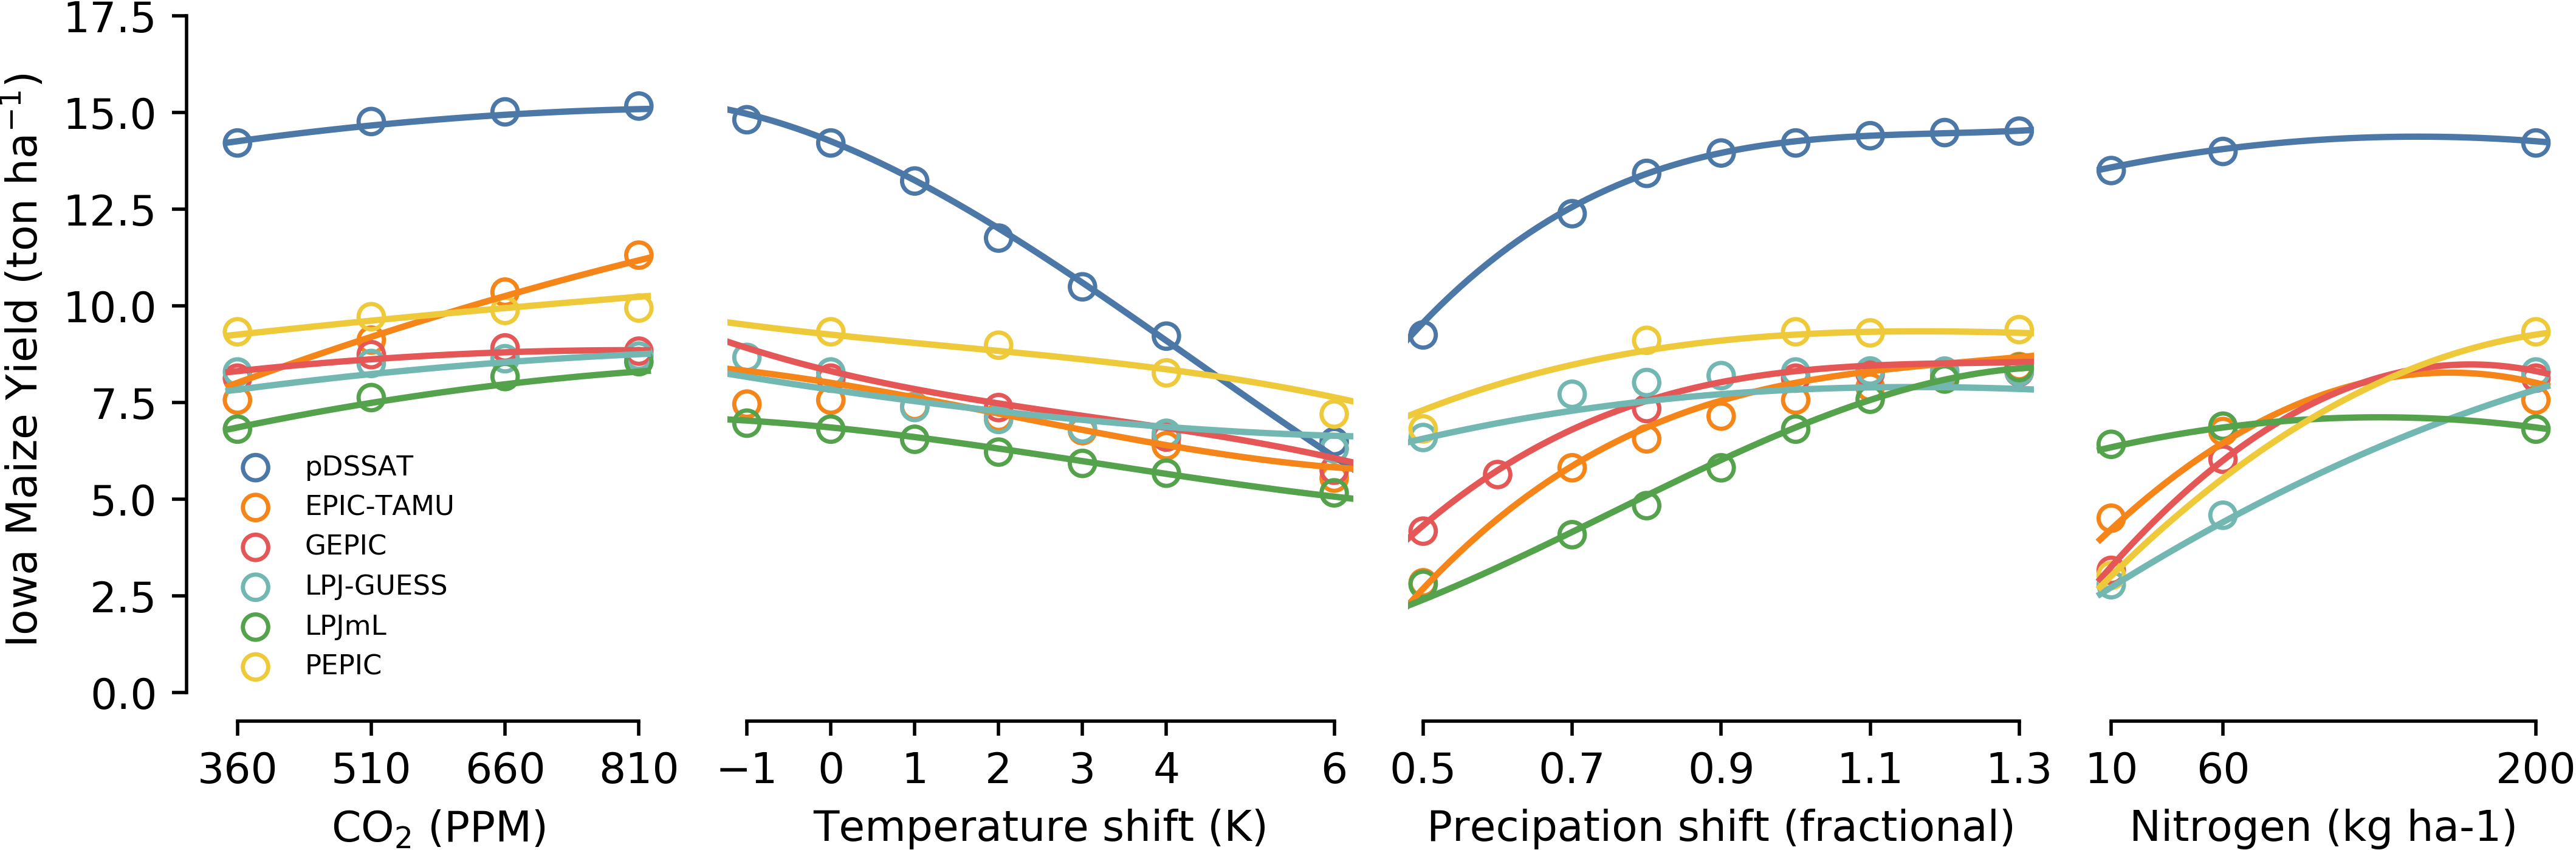
\includegraphics[width=16.3cm]{figures/regression_example_2.png}
    \caption{
    Illustration of variations in yield response across models, again successfully captured by the emulator. 
    Panels show simulations and emulations from six representative GGCMI models for rainfed maize in the same Iowa grid cell shown in Figure \ref{fig:regression}, with the same plot conventions. 
    Three models (PROMET, JULES, and CARAIB) that do not simulate the nitrogen dimension are omitted for clarity. 
    Models are uncalibrated, producing spread in absolute yields. 
	While most model responses can readily emulated with a simple polynomial, some response surfaces diverge slightly from the polynomial form, producing emulation error (e.g.\ LPJ-GUESS here, for all parameter dimensions), but 
    resulting error generally remains small relative to differences across models.
    }
   \label{fig:regression_2}
\end{figure*}

Yield responses to the four main drivers considered here (C, T, W, and N) are also quite diverse across locations, crops, and models, but in nearly all cases the local climatological mean responses are smooth enough to permit emulation with the functional form used here.
Figure \ref{fig:regression} illustrates geographic diversity of responses within a single crop and model, for rainfed maize in pDSSAT. While CO$_2$ responses (in t ha$^{-1}$/ppm) are quite similar, precipitation response is stronger in more arid locations and nitrogen responses appear strongly soil-dependent. This heterogeneity supports the choice of emulating at the grid cell level. 
In regions with current cultivation, yields evolve smoothly across the space sampled, and the polynomial fit captures the climatological-mean response to perturbations well. 
Emulators do perform poorly in a few regions that involve discontinuous or irregular yield responses. 
This condition is illustrated here with maize from the PROMET model in northern Canada, which is considered too cold for maize at present (0 ton ha$^{-1}$ yield), but which shows an abrupt rise to moderate yields once temperature rises by 4 degrees. 
Under these conditions, the 3rd order polynomial cannot fit the response, and errors are high. See Section \ref{S:4.1} for additional discussion. 

Crop yield responses in all models generally follow similar functional forms at any given location, though with a spread in magnitude (Figure \ref{fig:regression_2}, which shows rainfed maize in northern Iowa in a selection of GGCMI models). 
Absolute yield differences between models can be substantial because models are uncalibrated in some cases.
In general, models are most similar in their responses to temperature perturbations, and least similar to changes in CO$_2$. 
That is, CO$_2$ fertilization effects \textit{within} a single model are consistent across locations, but CO$_2$ effects differ strongly \textit{across} models. 
Differences in response shape can lead to some differences in the fidelity of emulation for different crop-model combinations; we evaluate these in more detail in the following section. 

Note that while the nitrogen dimension is important, it is also the most troublesome to emulate in this work because of its limited sampling compared to other dimensions. 
The GGCMI Phase II protocol specified only three nitrogen levels (10, 60 and 200 kg~N y$^{-1}$ ha$^{-1}$), so a third-order fit would be over-determined but a second-order fit can result in potentially unphysical results. 
Steep and nonlinear declines in yield with lower nitrogen levels mean that some regressions imply a peak in yield between the 100 and 200 kg~N y$^{-1}$ ha$^{-1}$ levels (Figure \ref{fig:regression_2}, right). 
While reduced yields under high nitrogen levels are physically possible and could reflect over-application at particular times in the growing period, they are implausible at the magnitude shown here and likely an artifact of the fit. 
The Bayesian Ridge estimator mitigates the `peak-decline effect' in the nitrogen dimension relative to ordinary least squares, but does not entirely remove it. 
The polynomial fit also cannot capture the well-documented saturation effect of nitrogen application \citep[e.g.][]{Torsten77} as accurately as would be possible with a non-parametric model. 

\subsection{Emulator performance metrics}
\label{S:4.1}
\begin{figure*}[ht]
\centering
    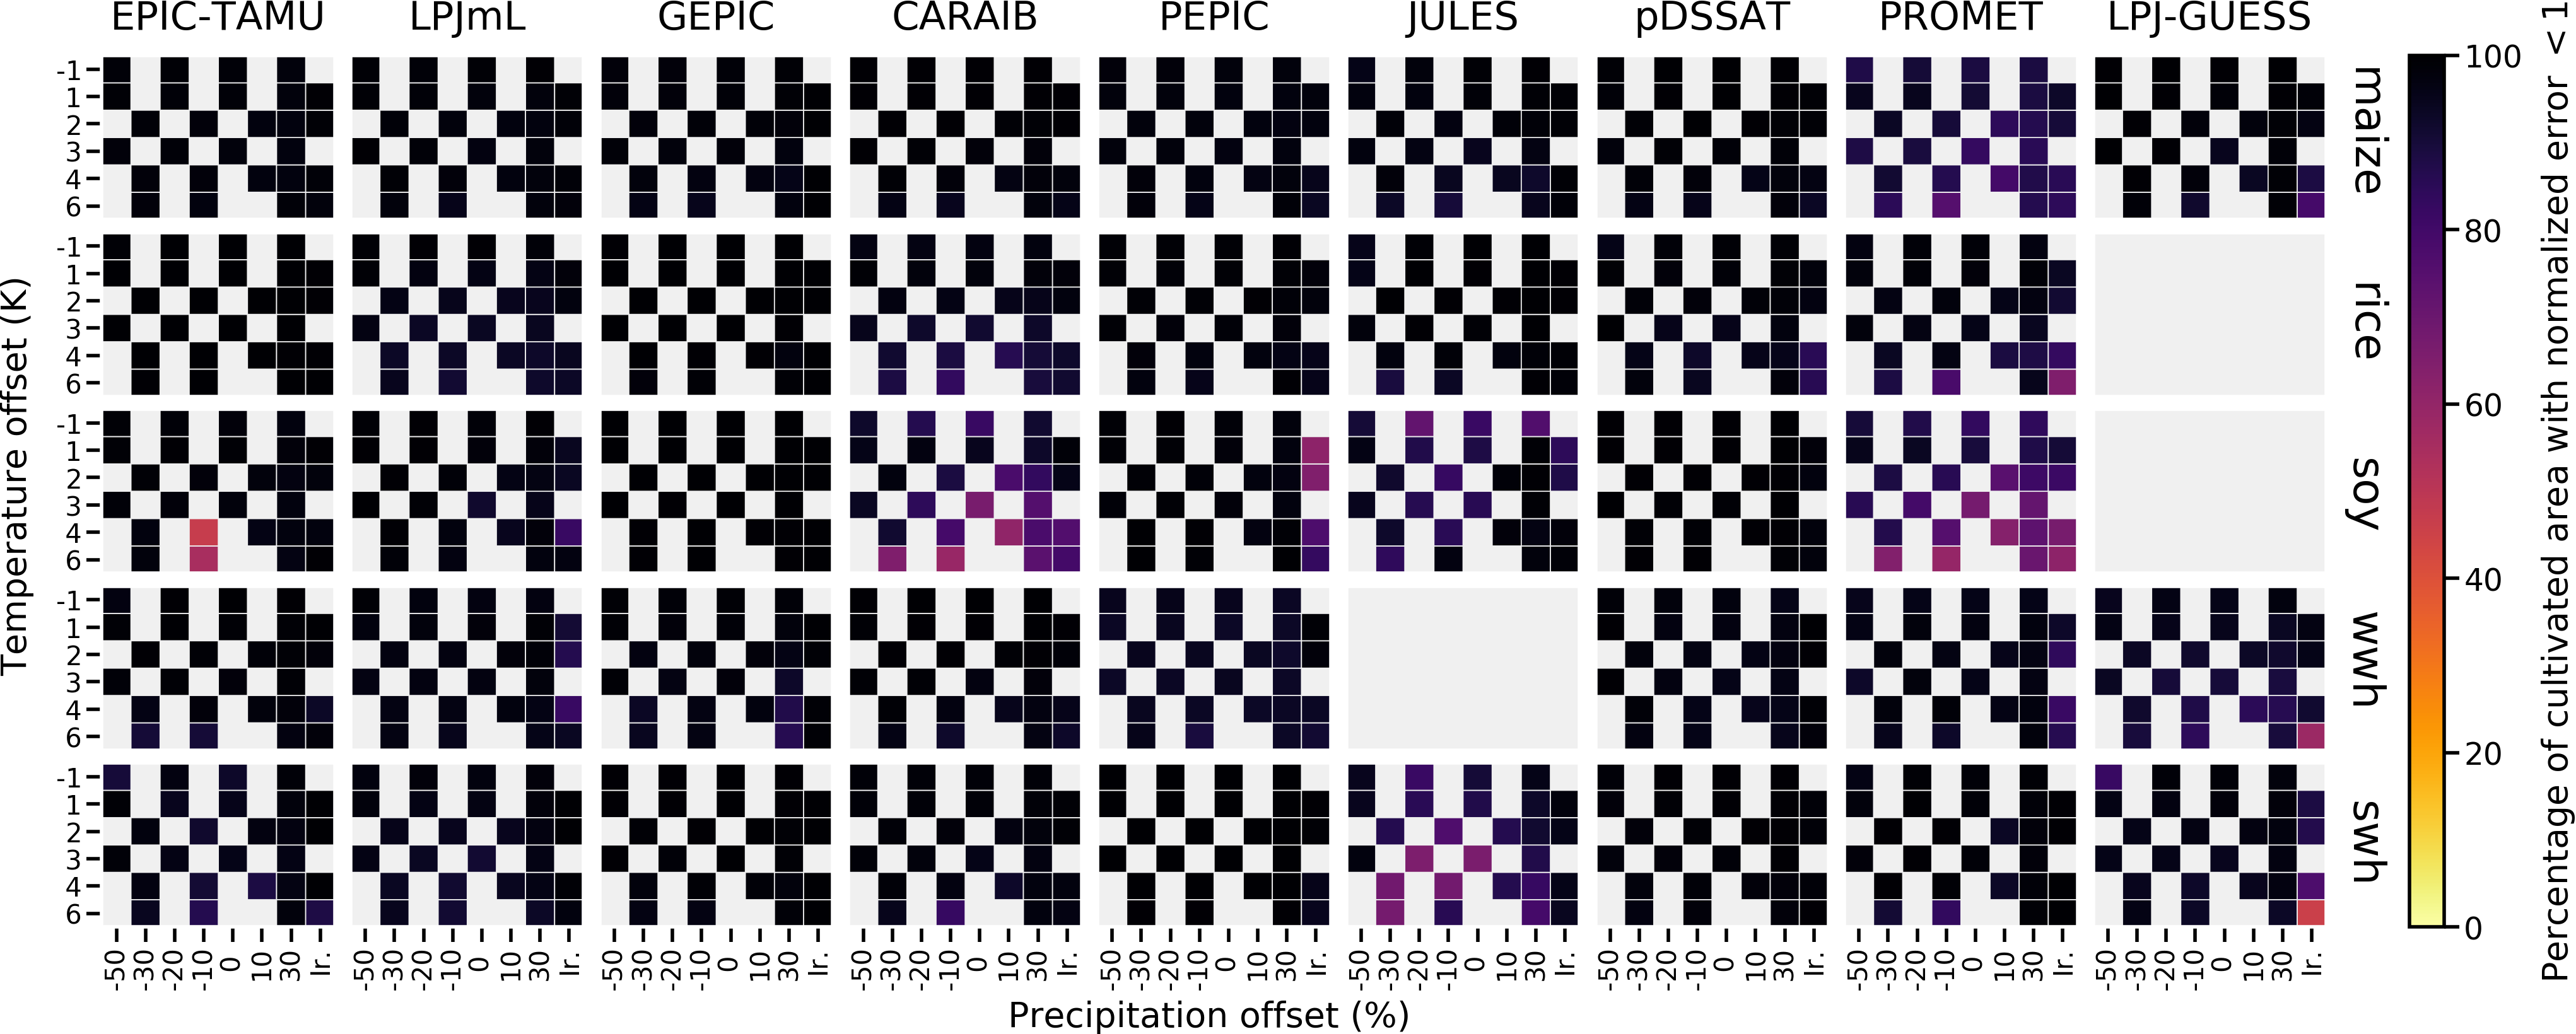
\includegraphics[width=16.3cm]{figures/error_grid_new.png}
    \caption{
    Assessment of emulator performance over currently cultivated areas based on normalized error (Equations \ref{eqn:error}). 
    We show performance of all 9 models emulated, over all crops and all sampled T and W inputs (``ir.'' indicates the irrigated W$_{\infty}$ setting), but with CO$_2$ and nitrogen held fixed at baseline values. 
    Large columns are crops and large rows models; squares within are T, W scenario pairs. 
    Colors denote the fraction of currently cultivated hectares (``area frac'') for each crop with normalized area $e$ less that 1 indicating the the error between the emulation and simulation less that one standard deviation of the ensemble simulation spread. 
    Of the possible 63 scenarios at a single CO$_2$ and N value, we consider only those for which all 9 (8 for rice, soybean, and winter wheat) models submitted data (Figure S1) so the model ensemble standard deviation can be calculated uniformly in each case. 
    JULES did not simulate winter wheat and LPJ-GUESS did not simulate rice and soybean. Emulator performance is generally satisfactory, with some exceptions. 
    Emulator failures (significant areas of poor performance) occur for individual crop-model combinations, with performance generally degrading for colder and wetter scenarios.
    }
   \label{fig:error_360}
\end{figure*}

\begin{figure*}[ht]
\centering
    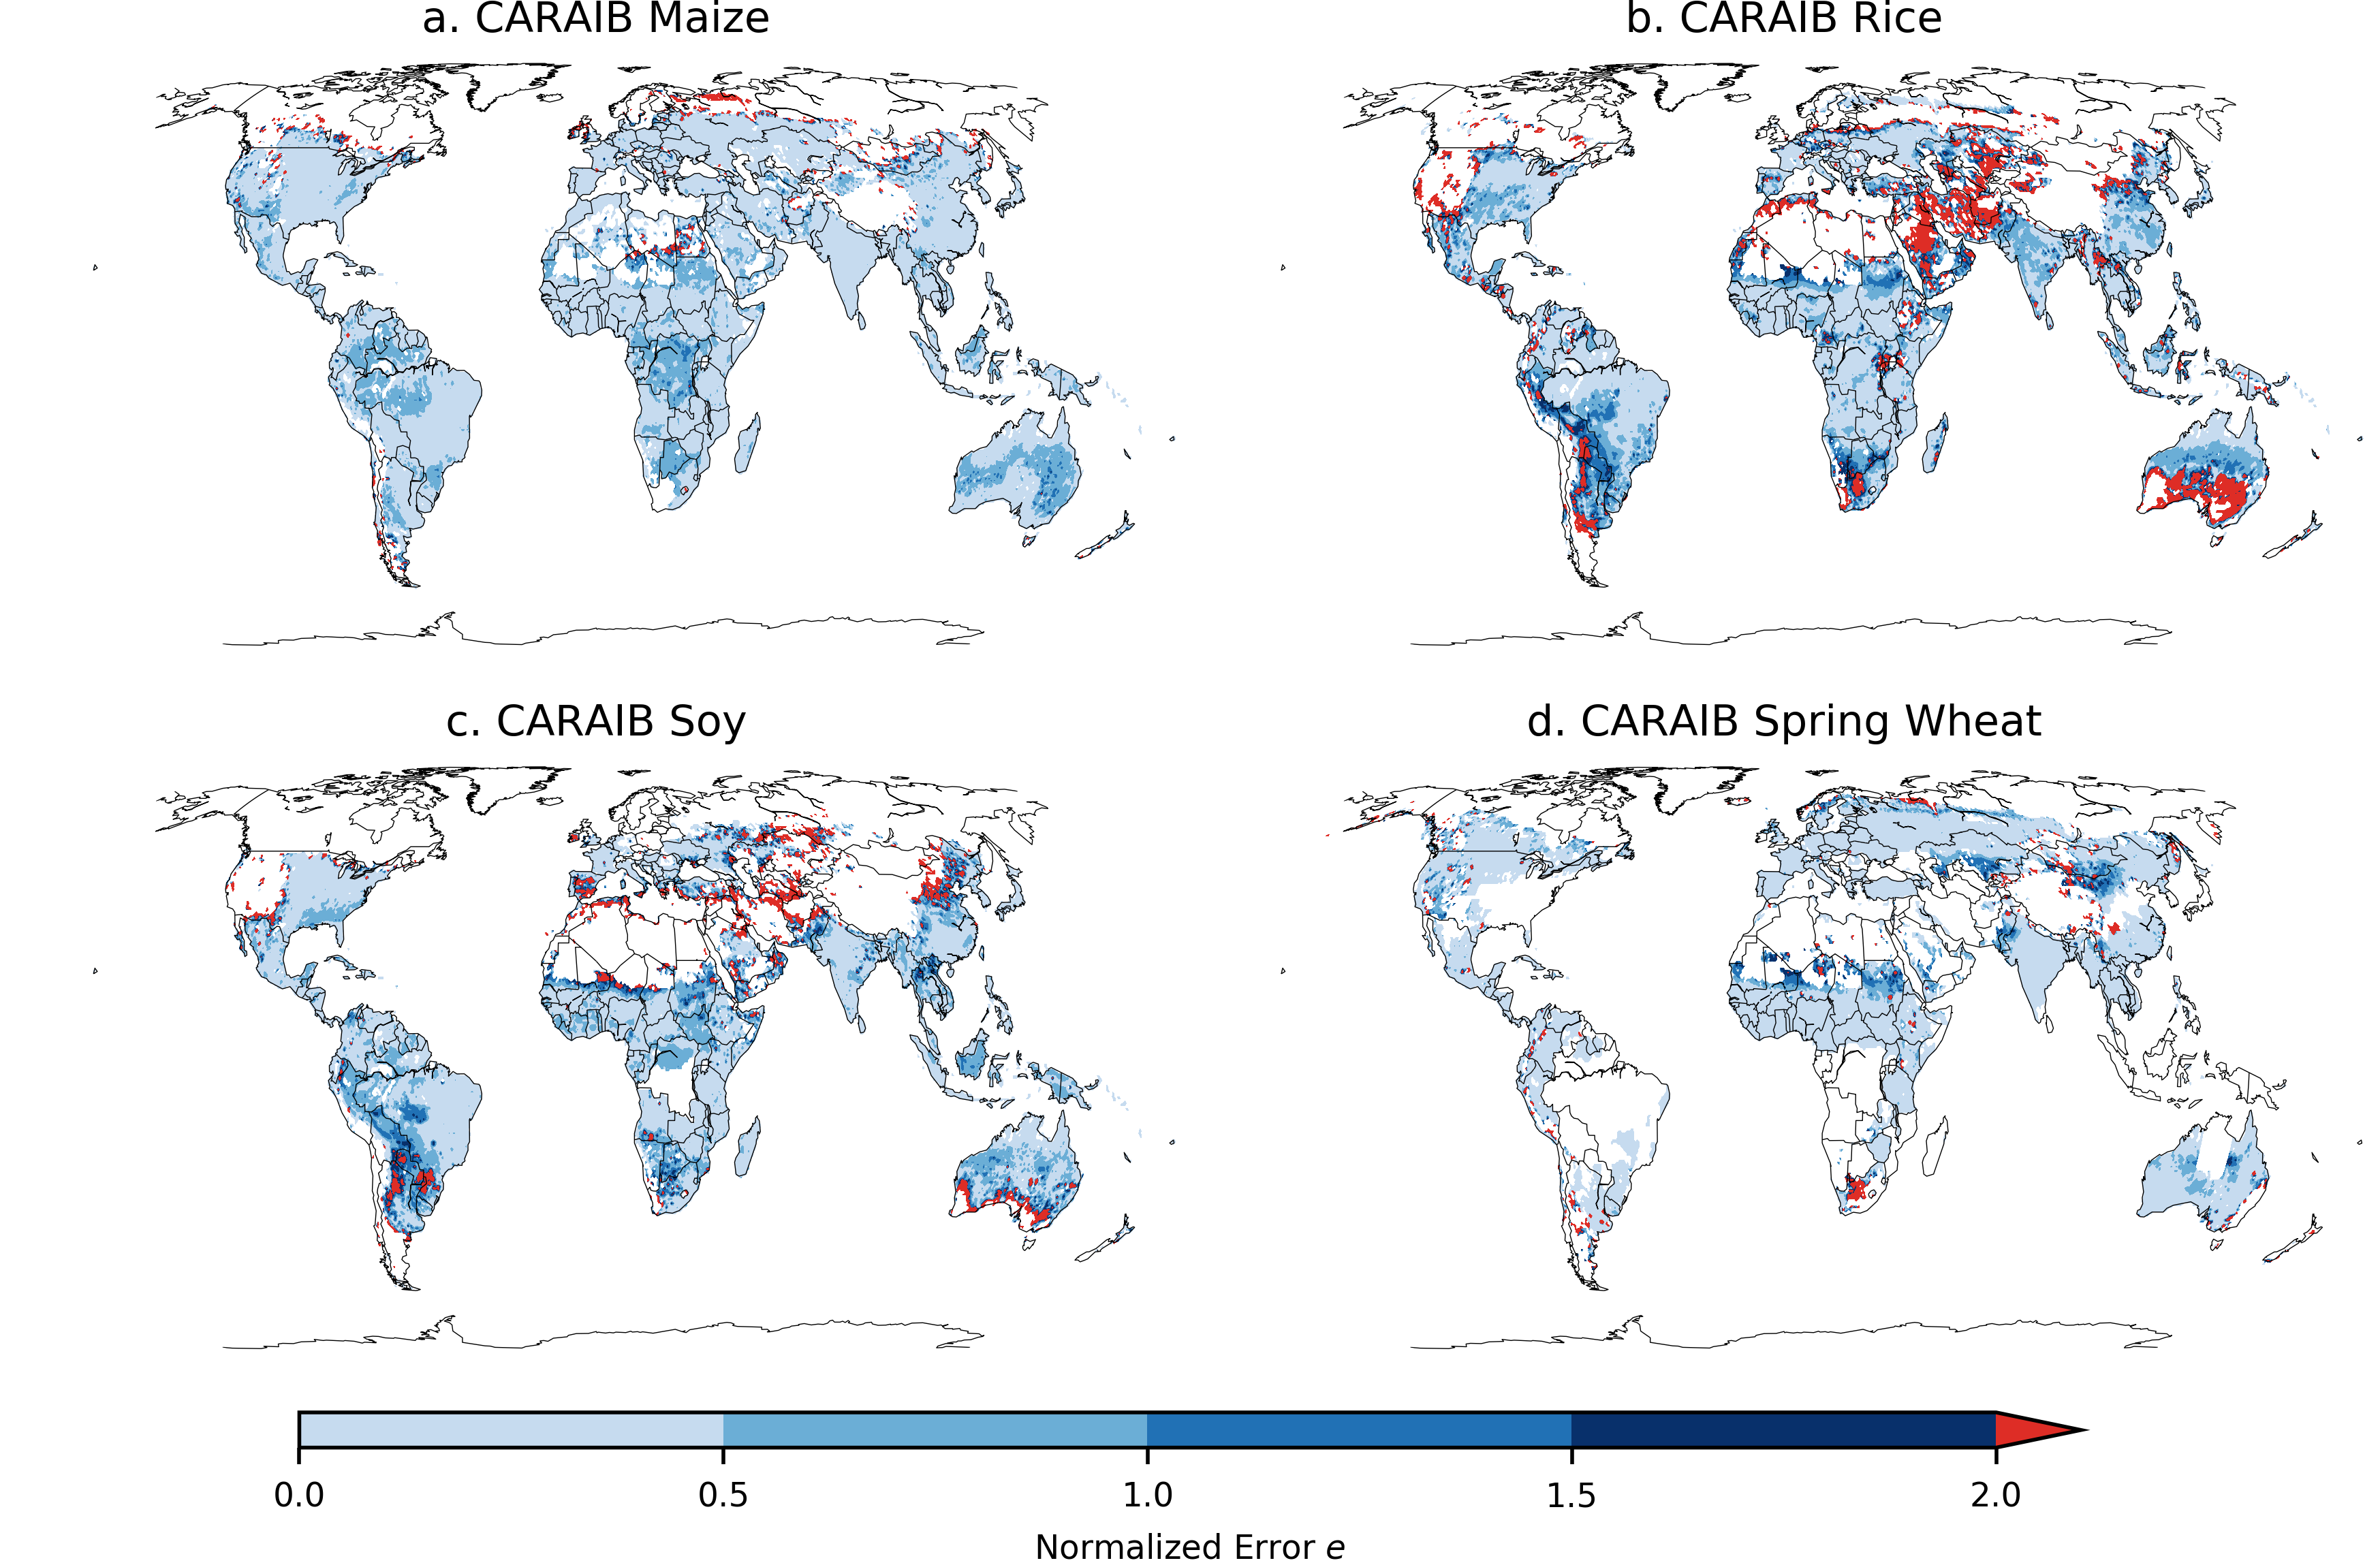
\includegraphics[width=16.3cm]{figures/CARAIB_spatial_error.png}
    \caption{
    Illustration of our first test of emulator performance, applied to the CARAIB model for the T+4 scenario for rainfed crops. 
    Colors indicate the normalized emulator error $e$, where $e > 1$ means that emulator error exceeds the multi-model standard deviation. 
    For consistency, we show $e$ only for geographic areas simulated by at least six models and where baseline yields are greater than 0.5 ton ha$^{-1}$.
    Emulator performance is generally good relative to model spread in areas where crops are currently cultivated (compare to Figure S2-S3) and in temperate zones in general; emulation issues occur primarily in marginal areas with low yield potentials. 
    }
   \label{fig:error}
\end{figure*}

Our emulators collectively consist of nearly 3 million individual regressions, so developing concise performance metrics poses a challenge.
No general agreed-upon criteria exist for defining an acceptable crop model emulator, so we present two different metrics, one relatively loose and one more stringent. 
These are described in detail below. Both metrics assess the ability of the emulator to reproduce model output from the GGCMI Phase II experiment. 
Finally, we also demonstrate the emulator's ability to reproduce a realistic projection of crop response to an evolving climate run. 

\smallskip
\textit{1. Normalized error.} We take as our first metric what we term the ``normalized error'', which compares the fidelity of an emulator to the inter-model spread. 
For a multi-model comparison exercise like GGCMI Phase II, a reasonable though loose emulator criterion is that its errors be small relative to intermodel differences. The normalized error $e$ is defined separately for each C,T,W,N scenario $s$ as the difference between emulated and simulated fractional yield changes, normalized by the standard deviation in simulated changes across all models: 

\begin{align}
	\hspace{10mm} e_{\: s}\  = \ & \frac{F_{em, \: s}-F_{sim, \: s}}{\sigma_{sim, \: s}}
	\intertext{where $F$ is the fractional change in yields $Y$ between scenario $s$ and baseline $b$:}
	\hspace{10mm} F_{\: s} \ = \ & \frac{Y_{s}-Y_{b}}{Y_{b}}
    \label{eqn:error}
\end{align}

Evaluation of this metric implies that GGCMI Phase II emulators are generally satisfactory. 
We calculate the mean error for each grid cell, model, and crop in each C,T,W,N scenario by comparing emulated and simulated yields, and show the averages over currently cultivated area in Figure \ref{fig:error}. 
A normalized error $e<1$ means that any deviation of the emulation from the simulation is less than 1 standard deviation of the inter-model spread.
Emulator performance is generally satisfactory. For maize, for example, all 9 models return $e < 1$ over 97\% of currently cultivated area. 
%and an additional 3 models produce $e < 1$ over 97\% of currently cultivated area. (LPJ-GUESS emulation is lowest in fidelity for maize, as previously shown in Figure \ref{fig:regression_2}, and produces 92\%.) 
Three crop model combinations produce $e < 1$ for less than 90\% of cultivated area: PROMET and CARAIB for soybeans (only 79\% and 83\% of cultivated area) JULES for spring wheat (85\% of cultivated area).
(See Supplemental Figures S10-S13 for examples of worst-case emulator failures for PROMET soy and JULES spring wheat.)
%In crop-model cases where performance is low, it tends to degrade most in the coldest and wettest scenarios, likely because yield increases are saturating in these conditions and cannot be captured with a 3rd order polynomial. 
Emulator performance will also be poor in cases where models show steep yield losses or complete crop failures.

While Figure \ref{fig:error_360} shows only currently cultivated land, performance can be worse in locations where crops are not currently cultivated, or on marginal lands where potential yields are low. (See Figures S14-S15 for analogous figures for all cultivated areas and for high CO$_2$.)
Figure \ref{fig:error} shows normalized error for CARAIB in the T+4 scenario over all simulated area that has non-zero baseline yield and at least 6 models providing simulations.  
Emulator performance can be poor ($e > 2$) in arid or mountainous zones -- the edges of the Sahara, the Near East, S.\ Africa and Southern Australia -- but is much better in regions where crops are grown. 
Over all-crop model combinations, the emulator produces $e < 1$ for 95\% of currently cultivated area and 98.5\% of all simulated area.
See Supplemental Figures S16-S22 for analogous figures for all models.

There is a trade off with number of terms included in the model specification. For example, pDSSAT maize, normalized error $e < 1$ for 98.8\% of currently cultivated land with the reduced statistical specification, and 98.3\% of currently cultivated land with all terms included in the emulator. Across all simulated land the value emulator skill increases with additional terms (from 94\% to 99\% of simulated area). In general, additional terms reduce errors in the aggregate, with large gains in emulator skill in ``fringe'' areas where crops are currently not cultivated and for certain models (JULES and PROMET). 

Note that the normalized error assessment is relatively forgiving for several reasons. 
First, it is an in-sample validation, with the emulation evaluated against the simulations actually used to train the emulator. 
Had we used a spline interpolation, the error would necessarily be zero. 
%(Our second metric involves evaluating on scenarios not included in the training set.)
Second, the metric scales emulator fidelity not by the magnitude of yield changes in the evaluated model but by the spread in yield changes across models. 
The normalized error $e$ for a given model then depends on the particular suite of other models considered in the intercomparison exercise.  
The rationale for the choice is to relate the fidelity of the emulation to the true uncertainty, which we take as the multi-model spread, but  
the metric then has the property that where models differ more widely, the standard for emulators becomes less stringent, and vice versa.
In GGCMI Phase II the effect is manifested in the higher normalized errors for soybeans across all models, which result not because soybean yields are difficult to emulate but because models agree more closely on yield changes for soybeans than for the other crops.

\smallskip
\textit{2. Out-of-sample validation.} We provide a second, more stringent test of emulator performance via a cross validation (also termed an out-of-sample validation). 
%In this test the GGCMI Phase II dataset is split randomly into two parts, with 66\% of the data used to train the model and the held-out 33\% used to test the fidelity of the resulting emulator.
In this test the GGCMI Phase II dataset is split randomly into two parts, with 90\% of the data used to train the model and the held-out 10\% used to test the fidelity of the resulting emulator.
We calculate the root mean square error (RMSE) between emulated (predicted) and actual simulated values across the test set, repeat the process twice and average the results of the two splits. 
The split does not represent a uniform number of samples in each location or in each model.
As a last step, we normalize the RMSE in each grid cell by dividing by its simulated yield change in the experiment sampling space in each gridcell.

\begin{table*}[hb]
    \caption{
    Root mean squared error of the emulator representation of a simulation as a percentage of baseline simulated yield change for the cross-validation process, for rainfed crops. Values are the mean grid cell error as a percentage of baseline yield, over all currently cultivated grid cells weighted by cultivation area. 
    Errors are calculated using the 90-10 cross validation scheme described in text, where the model is trained on 90\% of the data and validated on the held-out 10\% (repeated twice). 
    Values with * are cases where the OLS linear model fails. PEPIC has the lowest number of samples (n=121), so cannot be fit with the OLS and requires the Bayesian Ridge method.
    } 
    \label{table:ASE}
    \begin{tabular}{l | c | c | c | c | c} 
        \hline
        \textbf{Model}     & \textbf{Maize} & \textbf{Soybean} & \textbf{Rice} & \textbf{S. Wheat} & \textbf{W. Wheat} \\ \hline
        \textbf{CARAIB}    & 0.91 & 2.38 & 2.42 & 1.40  & 1.87    \\ \hline
        \textbf{EPIC-TAMU} & 1.76 & 2.55 & 1.60 & 1.94* & 1.12    \\ \hline
        \textbf{JULES}     & 2.64 & 4.02 & 1.70 & 2.15 & NA       \\ \hline
        \textbf{GEPIC}     & 2.40 & 1.25 & 2.13 & 3.29 & 2.89     \\ \hline
        \textbf{LPJ-GUESS} & 1.09 & NA   & NA   & 1.30 & 1.21     \\ \hline
        \textbf{LPJmL}     & 1.81 & 1.32 & 1.08 & 1.05 & 1.28     \\ \hline
        \textbf{pDSSAT}    & 1.72 & 1.13 & 1.57 & 1.27 & 1.51     \\ \hline
        \textbf{PROMET}    & 2.69 & 2.70 & 1.84 & 3.74 & 3.36     \\ \hline
        \textbf{PEPIC}     & 1.79* & 1.87* & 1.39 & 2.29* & 2.87* \\ \hline
    \end{tabular}
\end{table*}

The resulting error metric is generally low as a percentage of yield change.
Table \ref{table:ASE} shows the RMSE error over currently cultivated land for each model-crop combination for rainfed crops and include all simulations in CTWN space. 
Values are below 5\% for all cases.  
In absolute terms, mean grid cell root mean square errors (RMSE) weighted by cultivation area for rainfed crops are less than 0.2 ton ha$^{-1}$ for all cases except JULES soy (0.36 ton ha$^{-1}$).
Errors for irrigated emulators similar to the rainfed case, where the absolute errors are generally lower but are associated with yield changes that are also generally lower than the rainfed case.
Absolute global mean errors across all simulated grid cells (not weighted by cultivation area) are similar but not uniformly distributed across space. See Supplemental Figures S23-S34 for maps of cross validation error for each crop and model.

The metric of Table \ref{table:ASE} is relatively simple and can involve some biases. %We do not compare to yield \textit{changes};
The simple randomized sampling protocol for dividing training and test sets may mean that a training set omits edge simulations (those at the highest or lowest value of CTWN space). 
The test prediction then involves extrapolating out of the training set range (e.g.\ predicting a T+6 case when the training set extends only to T+4), an improper use of an emulator.
In this sense the metric is overly conservative, and values would be lower under a different sampling strategy (e.g.\ ``leave-one-out''). 
%The metric also does not relate emulation error to yield changes. 
For more detailed potential evaluation metrics see e.g.\ \citet{Castruccio14}.

\smallskip
\textit{3. Validation of emulation of realistic climate projections.}
\label{S:4.3}

\begin{figure*}[ht]
  \centering
  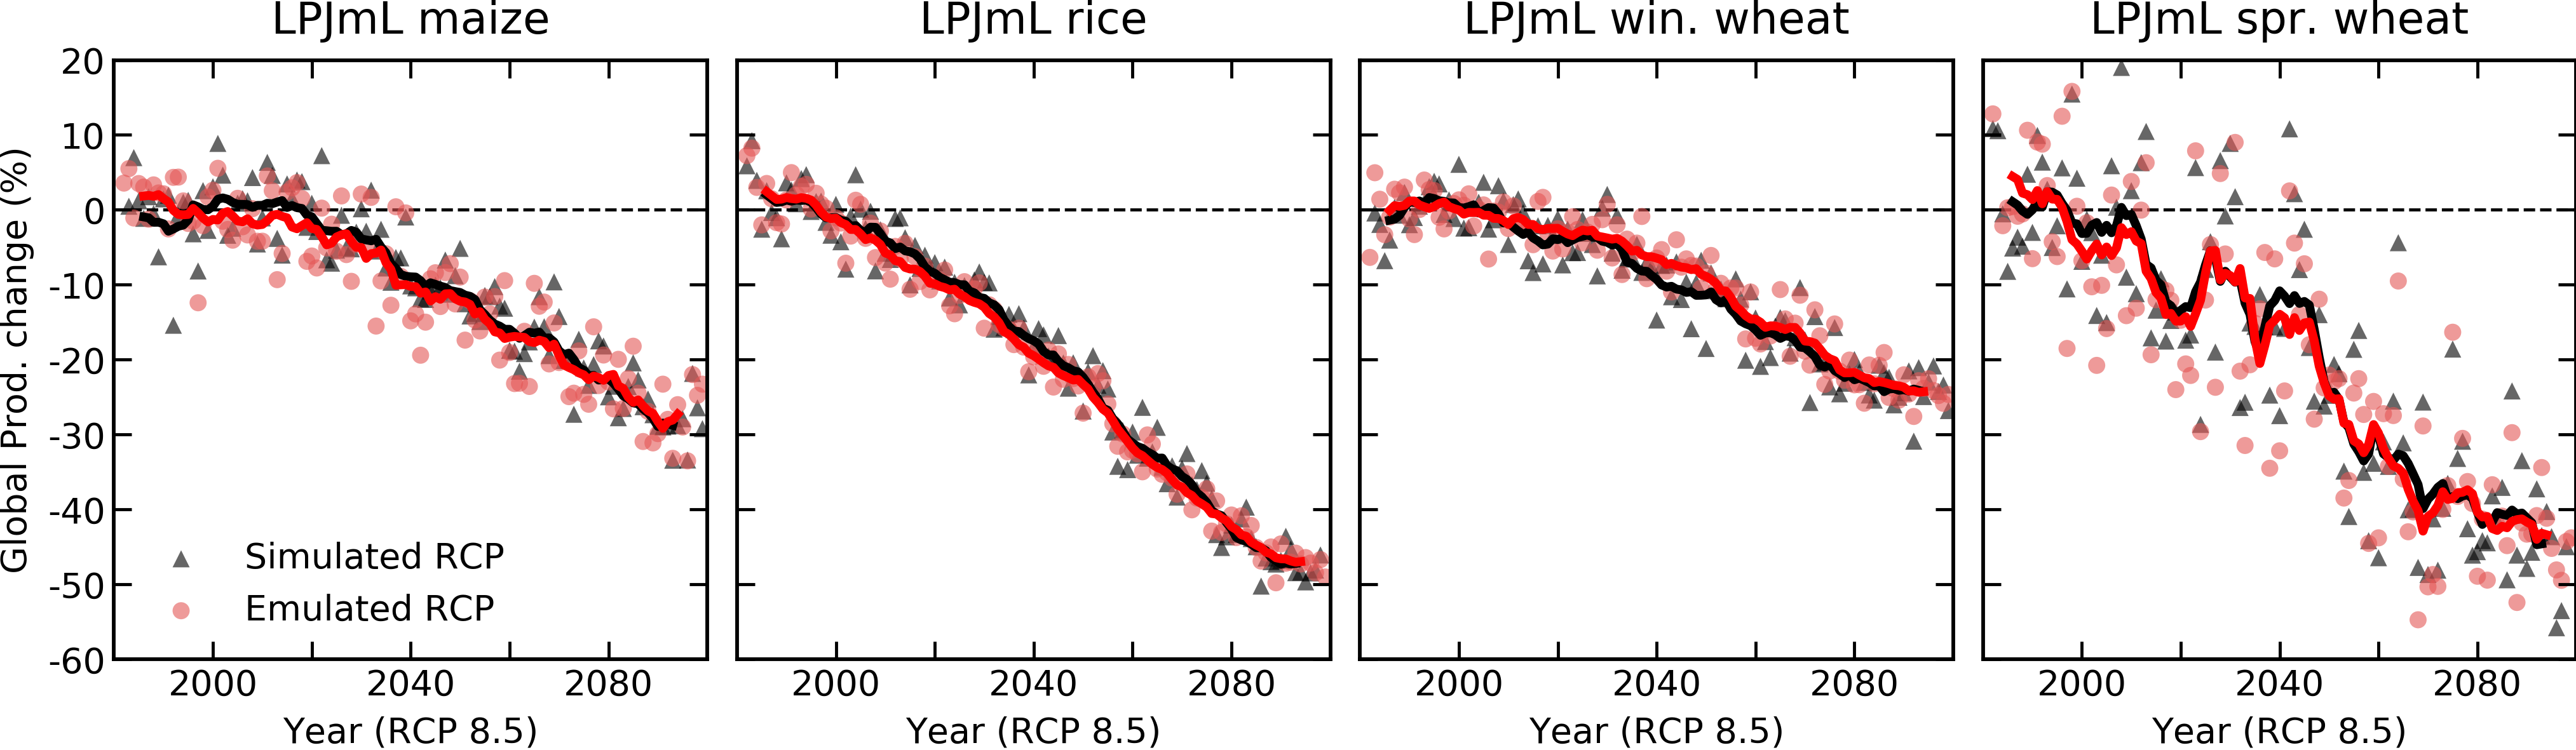
\includegraphics[width = 16.3cm]{figures/LPJMLRCP85comp.png}
  \caption{
  Test of emulator performance in reproducing yield simulations made with a realistic climate projection. 
  Panels show simulated (black) and emulated (red) global production for four crops from the LPJmL model, driven with temperature and precipitation outputs from the HADGEM2-ES climate model for the RCP8.5 scenario. In both cases nitrogen and CO$_2$ are held fixed at 200kg ha-1 and 360ppm.
  Points show yearly global production change from the 1980-2010 mean lines show 3rd order smoothed mean.
  The emulator trained on uniform climatological offset outputs is able to capture the general response under a transient climate run. 
  Those differences that are evident -- overestimation of some historical maize years, and muted response for winter wheat -- may be related to differences in baseline climates used.
  }
  \label{fig:lpjmlrcp}
\end{figure*}

Finally, we test the ability of an emulator based on the GGCMI Phase II perturbed mean training set to reproduce the response of a crop model driven by a realistic evolving climate scenario.
For the test, we drive the LPJmL crop model (representative among GGCMI Phase II models) with climate model output under the business-as-usual RCP 8.5 scenario.
We choose for this purpose a climate model with relatively high changes in growing-season temperature variability relative to other models in the Coupled Model Intercomparison Project Phase 5 (CMIP-5) archive, HADGEM2-ES \citep{Jones2011h}. (See Supplemental Figure S35.)
We then drive the LPJmL emulator with the climatological anomalies for precipitation and temperature calculated from the HADGEM2-ES output. 
The resulting emulated yields reliably reproduce simulated yields under the full climate scenario (Figure \ref{fig:lpjmlrcp}). 

\textcolor{red}{XX needs edits from here on} The ability of our emulator to capture ... suggests that the temperature distribution in a location within the growing season is relatively insignificant when compared to the mean change on longer timescales. 
The year-to-year emulation does not match the yearly simulated values (Figure \ref{fig:lpjmlrcp}, points) as well as the climatological mean (Figure \ref{fig:lpjmlrcp}, lines), indicating the importance of the growing season temperature distribution at the yearly time scale. 
We do not intend the emulator to be used to project yearly yields.
The three potential causes for remaining differences are as follows.
First, the growing season used for calculating the temperature and precipitation changes in the climate model run in especially important here because growing seasons vary dynamically in models based on temperature. 
In the case shown here, using the growing seasons from the baseline GGCMI Phase II simulations provides the best result because the emulator implicitly includes the crop model response to changing growing season. 
If the growing season from the RCP crop model is utilized (an unrealistic use-case because these simulations do not exist for every possible emulator application) you are likely to over- or under-estimate the growing season temperature or precipitation changes depending on the seasonality of weather in the growing season. 
Second, the baseline climate product used in each case have different precipitation and temperature representations including potentially important differences in distributions in the historical P and T. 
For example baseline (1980-2010) production in the phase II simulation is 7\% lower than baseline production in the RCP simulation for winter wheat. 
(The emulator will never be able to capture these differences in baseline production.)
Third, missed relevant changes in distributions in precipitation and temperature at the climatological-mean timescale.
We expect relevant changes in distributions and growing seasons to have the biggest impact for winter wheat.

%%%%%%%%%%%%%%%%%%%%%%%%%%%%%%%%%%%%%%%%%%%%%%%%%%%%%%%%%%%%%%%
%%%%%%%%%%%%%%%%%%%%%%%%%%%%%%%%%%%%%%%%%%%%%%%%%%%%%%%%%%%%%%%
\section{Emulator results and products}
\label{S:5}
\begin{figure*}[ht]
  \centering
  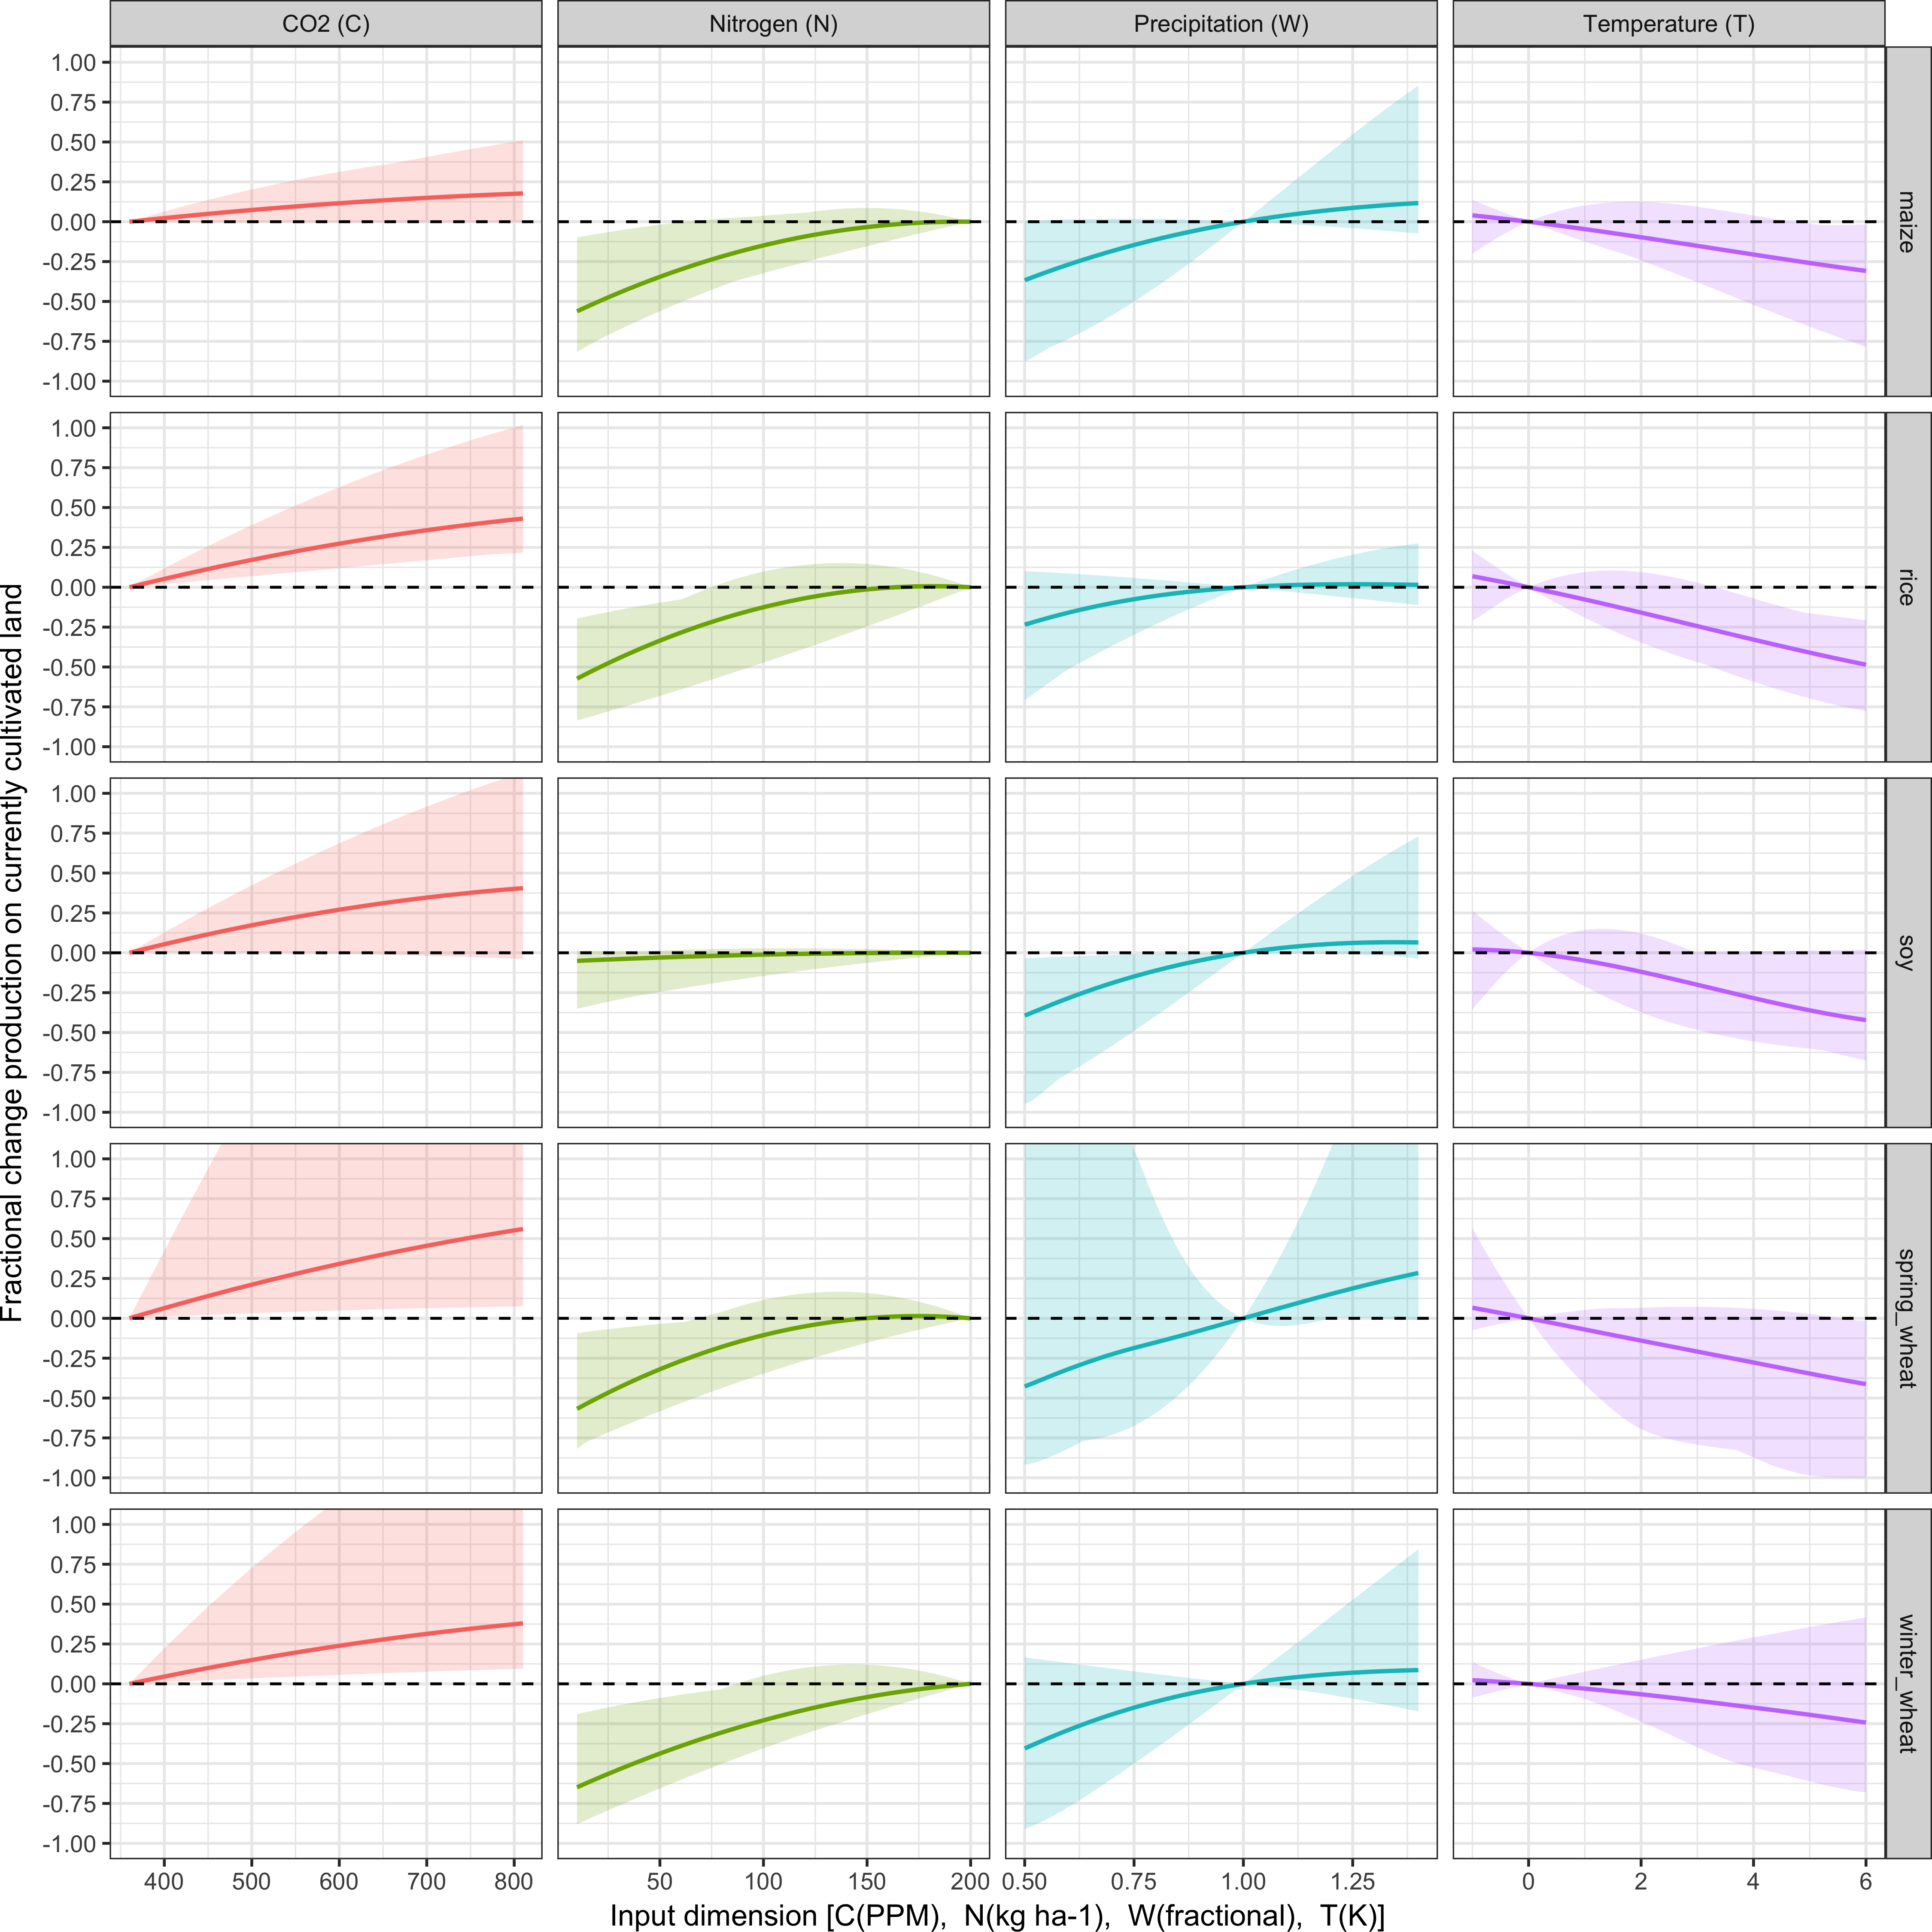
\includegraphics[width = 16.3cm]{figures/em_CTWN_all_crops.png}
  \caption{
  Emulated global damage functions for the five crops included in GGCMI Phase II for the four dimensions varied: CO$_2$, temperature, water, and nitrogen (collectively ``CTWN''). 
  Black line shows the multi-model ensemble mean and the shaded area and colored lines show the individual model projections. 
  All other covariates held constant at baseline values (T+0K, W+0\%, C = 360ppm, and N = 200kg ha-1). 
  Damages are reported as percent change in global production relative to the baseline (1980-2010) case over currently cultivated land.
  }
  \label{fig:all_dims}
\end{figure*}

Because the emulator or ``surrogate model'' transforms the discrete simulation samples into a continuous response surface at any geographic scale, it can be used for a variety of applications, including construction of continuous damage functions in a flexible format. 
As an example, we present global damage functions constructed from the 4D emulation, for all four dimensions tested in this study (Figure \ref{fig:all_dims}) with the ensemble median and ensemble spread shown in bold line and ribbon. 
This is helpful in the crop model intercomparison project context for diagnosing model differences. 
In general, across model spread is qualitatively similar across different crops and different dimensions with some notable exceptions. 
Model spread is highest for spring wheat in general across all dimensions.
Maize has a muted response to CO$_2$ as a C4 plant, and the impacts of temperature are most consistent for soybeans (see also Figure \ref{fig:error_360}).
Increased precipitation does little to increase global production for all crops except spring wheat, and rice is not generally grown in water-limited conditions so it shows the weakest response to reductions in precipitation.
The nitrogen response is relatively consistent across crops, with most models showing saturation at values less that 200 kg ha$^{-1}$, except for soybeans, an efficient atmospheric nitrogen-fixer.

Note that these functions are presented here in Figure \ref{fig:all_dims} only as examples and do not represent true global projections, because they are developed from simulation data with a uniform temperature shift while increases in global mean temperature should manifest non-uniformly in space and distributions \citep[e.g][]{Sippel2015}. 
The global coverage of the GGCMI Phase II simulations allows impacts modelers to apply arbitrary geographically-varying climate projections, as well as arbitrary aggregation masks, to develop damage functions for any climate scenario and any geopolitical or geographic level bigger than 0.5 degrees in latitude and longitude. 

\begin{figure*}[ht]
    \centering
    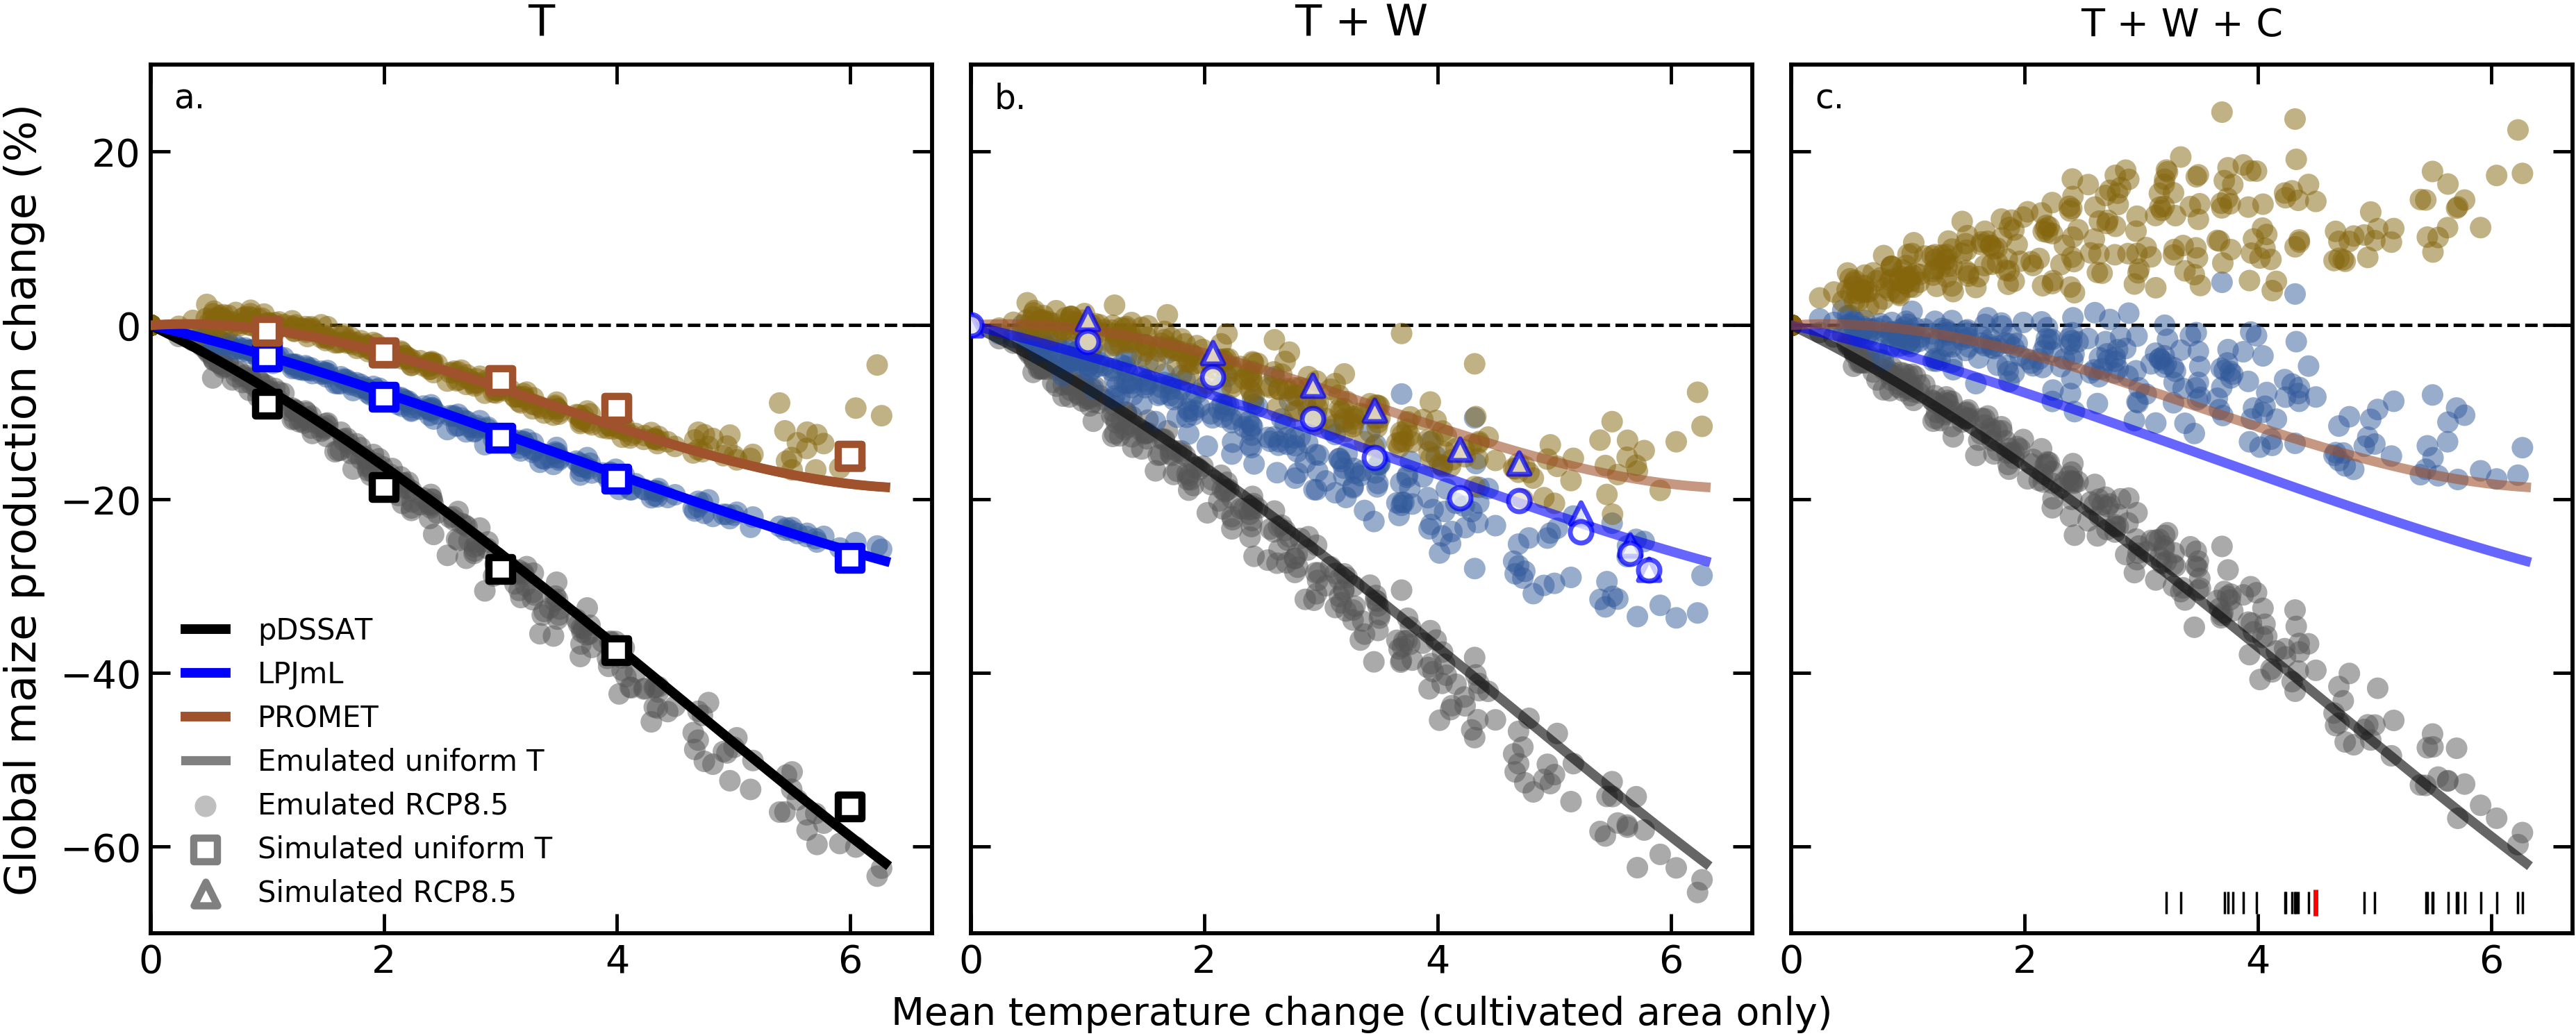
\includegraphics[width = 16.3cm]{figures/global_em_maize.png}
    \caption{
    Illustration of the effects of factors affecting yields in more realistic climate scenarios. 
    Figure shows emulated yield changes for maize on currently cultivated land under RCP8.5 (relative to 1980-2010 mean) for three representative crop models, with changes to T only (\textbf{a}), to T and W (\textbf{b}), and to T, W, and CO$_2$ (\textbf{c}).
    Circles are emulated yearly global production changes for 2010-2100 in scenarios from 5 CMIP-5 climate models, i.e.\ 490 total per crop model, with x-axis the mean T shift over all grid cells where maize are grown (unweighted by within-cell cultivated area). %Rug plot at bottom shows range of final (mean 2090-2100) temperatures across climate models.
    Bold lines are the emulated values over uniform T shifts. 
    Open squares in panel \textbf{a} are GGCMI Phase II simulated values for each T level (with CWN at baseline).  
    Emulations capture simulated behavior well (compare squares to lines), with the exception of PROMET at extreme temperature change. (See also Figure \ref{fig:regression}.)
    Mean yields are very similar whether T changes occur as a uniform temperature shift or in a more realistic spatial pattern (compare lines to circles). 
    \textbf{b:} adding in projected precipitation changes depresses yields slightly for PROMET and increases spread between projections for a given temperature change for the other models. 
    \textbf{c:} adding in CO$_2$ changes produces very different responses across models. 
    CO$_2$ fertilization is small in pDSSAT, moderate in LPJmL, and very large in PROMET. 
    Emulation uncertainty is small compared to the differences across climate and crop models.
    Square points show the T+6,C=810ppm phase II simulated production change values.
    }
    \label{fig:globe_em}
\end{figure*}

The emulator can also be used for investigating the contributions of the different major climate drivers to production outcomes as it can project many different climate scenarios or models quickly.
The emulated crop model yield responses to a high-end climate change scenario (Representative Concentration Pathway (RCP) 8.5) are shown in Figure \ref{fig:globe_em} for 5 climate models from the CMIP-5 archive \citep{Taylor2012} at the yearly scale. 

The differences between the emulation and the simulations for a uniform T shift are small compared to the differences across different crop models.
PROMET, the most quantitatively difficult models to emulate for maize, is shown in Figure \ref{fig:globe_em} to illustrate that emulation error at the global production scale is still small compared to the spread across crop models or the spread across climate projections when all factors are included.
The uniform temperature shift over growing area is not very different from realistic scenarios (though it biases LPJmL low). 
That is, projected temperature change distribution in space do not matter that much over currently cultivated area, but are likely important to production in high latitude regions which will warm much faster than lower latitudes.

Precipitation changes introduce some noise because different climate models have different P response for a given temperature change. 
PROMET shows a near uniform reduction in yields with precipitation effects included.
Including the direct effects of elevated CO$_2$ introduces the largest intermodel uncertainty with different crop models showing very different responses. 
This difference in model response to CO$_2$ is much larger than differences resulting from different climate model sensitivity to CO$_2$ (T(CO$_2$)).
Individual climate model sensitives can be seen in the separation in the PROMET response to CO$_2$.
Emulation based on GGCMI climatological mean shifts is useful for realistic scenarios and emulator errors are small compared to climate model differences and tiny compared to crop model differences.

%Finally, the emulator constructed from the GGCMI perturbed mean training set reliably reproduces a realistic RCP scenario indicating that the temperature distribution in a location within the growing season is relatively insignificant when compared to the mean change.
%First, the spatial pattern of temperature change under a realistic climate scenario is relatively insignificant at the global mean production level.
%Second, the spread across climate model response increases considerably with precipitation changes and CO$_2$ effects included, with precipitation changes reducing production and CO$_2$ increasing it.
%The CO$_2$ response is more heterogeneous across crop models that precipitation changes for maize. 
%The globally gridded nature of the emulator allows for easy analysis at almost any spatial scale.
%Note that no direct comparison to the simulations is possible in cases b or c.
%Finally, the emulator can be used to quickly project crop yield responses to climate change under a variety of conditions. 

%%%%%%%%%%%%%%%%%%%%%%%%%%%%%%%%%%%%%%%%%%%%%%%%%%%%%%%%%%%%%%%
%%%%%%%%%%%%%%%%%%%%%%%%%%%%%%%%%%%%%%%%%%%%%%%%%%%%%%%%%%%%%%%
\section{Discussion and conclusions} 
\label{S:6}
We show that the systematic parameter sampling in the GGCMI Phase II experiments allow emulating climatological crop yield responses with a relatively simple reduced-form statistical model. 
The sampling provides information on the influence of multiple interacting factors in a way that realistic climate model simulations cannot, and allows isolating long-term impacts from confounding factors that lead to different year-over-year responses. 
The use of a relatively simple functional form in turn offers the possibility of physical interpretation of parameter values that can assist in model intercomparison and evaluation. 
The yield output for a single GGCMI Phase II model that simulates all scenarios and all five crops is $\sim$12.5 GB; the emulator is $\sim$20 MB, a reduction of nearly three orders of magnitude.
One-thousand years of global 0.5 degree yields (appropriately 40,000 locations) can be emulated in 20 seconds on a laptop computer. 

Several cautions should be noted when using the emulator. 
While the emulator allows estimating agricultural impacts under arbitrary climate scenarios, extrapolation outside the sample space should be avoided. 
Emulators by design reduce the complexity of process-based simulations and can thus deviate from the raw simulation output. 
This limitation is especially prominent in models with limited sampling or in geographic regions outside the current cultivated area.
Additionally, because the simulation protocol was designed to focus on change in yield under climate perturbations and not on replicating real-world yields, the models are not formally calibrated so they should not be used for impacts projections of absolute yields except in conjunction with historical yield information. 
Finally, because the GGCMI Phase II simulations apply uniform perturbations to historical climate inputs, they do not sample potential changes in climate variability. 
\textcolor{red}{but this only matters so much... but we have not not tested in all the crop models or across all climate models}
Although such changes are uncertain and remain poorly characterized \citep[e.g.][]{Alexande2006, Kodra2014}, follow-up experiments may wish to consider them. 
Several recent studies have described procedures for generating simulations that combine historical data with model projections of changes in the marginal distributions or temporal dependence of temperature and precipitation (e.g.\ \citet{Leeds2015, poppick2016, Won16} and \citet{Haugen2018}).

The GGCMI Phase II dataset invites a broad range of potential future avenues of analysis, especially because emulation allows statistical distillation of the large dataset (40 billion simulated yields) into a tractable form. 
Potential studies might include a detailed examination of interaction terms between the major input drivers, robust quantification of model sensitivities to input drivers, exploration of yield responses to extremes, and evaluation of geographic shifts in optimal growing regions. 
The dataset also enables studies of emulation itself, including a more systematic evaluation of different statistical and machine learning model specifications.
In general, the development of multi-model ensembles involving systematic parameters sweeps has large promise for better understanding potential future crop responses and for improving process-based crop models.

%%%%%%%%%%%%%%%%%%%%%%%%%%%%%%%%%%%%%%%%%%%%%%%%%%%%%%%%%%%%%%%
\codedataavailability{The polynomial emulator parameter matrices for all crop model emulators are available at {doi.org/XXXXX}}

%\appendix
%\section{}
%\subsection{Data Access}
%\noappendix %% use this to mark the end of the appendix section

\authorcontribution{J.E., C.M, A.R., J.F., and E.M.\ designed the research. C.M., J.J., P.F., C.F., L.F., R.C.I., I.J., C.J., W.L., S.O., M.P., T.P., A.Re., K.W., and F.Z.\ performed the simulations. J.F., J.J., A.S., M.L., Z.W., and E.M.\ performed the analysis and J.F., C.M., and E.M.\ prepared the manuscript.}

\competinginterests{The authors declare no competing interests.}

\begin{acknowledgements}
We thank Michael Stein and Kevin Schwarzwald, who provided helpful suggestions that contributed to this work. 
This research was performed as part of the Center for Robust Decision-making on Climate and Energy Policy (RDCEP) at the University of Chicago, and was supported through a variety of sources. 
RDCEP is funded by NSF grant \#SES-1463644 through the Decision Making Under Uncertainty program. 
J.F.\ was supported by the NSF NRT program, grant \#DGE-1735359 and by an NSF Graduate Research Fellowship, grant \#DGE-1746045. 
C.M.\ was supported by the MACMIT project (01LN1317A) funded through the German Federal Ministry of Education and Research (BMBF). 
C.F.\ was supported by the European Research Council Synergy grant \#ERC-2013-SynG-610028 Imbalance-P. 
P.F.\ and K.W.\ were supported  by the Newton Fund through the Met Office Climate Science for Service Partnership Brazil (CSSP Brazil). 
K.W.\ was supported by the IMPREX research project supported by the European Commission under the Horizon 2020 Framework programme, grant \#641811. 
A.S.\ was supported by the Office of Science of the U.S.\ Department of Energy as part of the Multi-sector Dynamics Research Program Area. 
S.O.\ acknowledges support from the Swedish strong research areas BECC and MERGE together with support from LUCCI (Lund University Centre for studies of Carbon Cycle and Climate Interactions). 
R.C.I.\ acknowledges support from the Texas Agrilife Research and Extension, Texas A \& M University. 
This is paper number 35 of the Birmingham Institute of Forest Research. 
Computing resources were provided by the University of Chicago Research Computing Center (RCC).
\vspace{1cm}
\textit{This material is based upon work supported by the National Science Foundation Graduate Research Fellowship Program under Grant No. (DGE-1746045). 
Any opinions, findings, and conclusions or recommendations expressed in this material are those of the authors and do not necessarily reflect the views of the National Science Foundation.}
\end{acknowledgements}

\bibliographystyle{copernicus}
\bibliography{bib}

\end{document}

%%%%%%%%%%%%%%%%%%%%%%%%%%%%%%%%%%%%%%%%%%%%%%%%%%%%%%%%%%%%%%%

%%%%%%%%%%%%%%%%%%%%%%%%%%%%%%%%%%%%%%%%%%%%%%%%%%%%%%%%%%%%%%%

%%%%%%%%%%%%%%%%%%%%%%%%%%%%%%%%%%%%%%%%%%%%%%%%%%%%%%%%%%%%%%%

%%%%%%%%%%%%%%%%%%%%%%%%%%%%%%%%%%%%%%%%%%%%%%%%%%%%%%%%%%%%%%%

%%%%%%%%%%%%%%%%%%%%%%%%%%%%%%%%%%%%%%%%%%%%%%%%%%%%%%%%%%%%%%%

\begin{table*}[hb]
    \caption{
        Mean squared error of emulator representation of a simulation as a percentage of baseline simulated yield for the cross-validation process, for rainfed and irrigated (parentheses) crops. Values are the median grid cell error as a percentage of baseline yield, over all currently cultivated grid cells with baseline yield $>$ 0.5 ton ha$^{-1}$. (We mask lower-yield locations because they are especially problematic in a yield-normalized metric.) % minor disparities result in high errors. 
        Errors are calculated using the 3-fold stratified k-fold cross validation scheme described in text, where the model is trained on 66\% of the data and validated on the held-out 33\% (repeated three times). 
        Emulator errors considered unacceptable are highlighted in bold. 
        Values with * are cases where the OLS linear model fails. PEPIC has the lowest number of samples (n=121), so cannot be fit with the OLS and requires the Bayesian Ridge method.
    } 
    \label{table:ASE}
    \begin{tabular}{l | c | c | c | c | c} 
        \hline
        \textbf{Model}     & \textbf{Maize} & \textbf{Soybean} & \textbf{Rice} & \textbf{S. Wheat} & \textbf{W. Wheat} \\ \hline
        \textbf{CARAIB}    & 0.45 (0.35) & 1.22 (0.50) & 1.67 (0.32) & 0.48 (0.26) & 1.21 (0.47) \\ \hline
        \textbf{EPIC-TAMU} & 2.08 (0.61) & 4.59 (0.20) & 0.74 (0.27) & 2.81* (0.20) & 1.34 (0.14)  \\ \hline
        \textbf{JULES}     & \textbf{7.46} (0.03) & \textbf{27.0} (10.21)& \textbf{11.7} (0.23) & \textbf{19.0} (5.23)  & NA  \\ \hline
        \textbf{GEPIC}     & 3.13 (0.18) & 1.35 (0.20) & 3.12 (0.36) & 2.28 (0.13) & 3.55 (0.20) \\ \hline
        \textbf{LPJ-GUESS} & 0.66 (0.85) & NA    & NA  & 1.13 (2.83) & 0.67 (0.98)                        \\ \hline
        \textbf{LPJmL}     & 2.04 (0.14) & 1.52 (0.24) & 1.09 (0.22) & 0.51 (0.20) & 0.65 (0.22)           \\ \hline
        \textbf{pDSSAT}    & 2.82 (0.52) & 2.30 (0.25) & 3.85 (2.30) & 0.51 (0.20) & 3.27 (0.97)            \\ \hline
        \textbf{PROMET}    & 2.45 (0.30) & 2.96 (1.91) & \textbf{11.8} (1.87) & 4.98 (0.13) & 4.47 (0.21)  \\ \hline
        \textbf{PEPIC}     & 2.04* (0.79) & 0.82* (3.27) & 1.21* (1.82) & 1.25* (0.54) & 4.33* (0.51)      \\ \hline
    \end{tabular}
\end{table*}

%\textcolor{red}{thisis one ref I found but it may not be the best reference and if we drop the claim of "weeks or even months" we can probably also do without a citation here...}
%Previous studies have suggested that in all but very arid regions, yields are not sensitive to how precipitation is distributed within a month \citep{Glotter14} although the impact of precipitation distribution within a crop season can be significant \citep{CHALLINOR200499}. 

%(Equations \ref{eqn:per_yield} and  \ref{eqn:error}). 
%for a is to ask whether is what we term the ``normalized error'', which compares the fidelity of an emulator for a given model and scenario to the inter-model uncertainty. 

%Note that 
%The emulator fails when the yield response has a discontinuity or is irregular in some regard. 
%For example, some simulation models report no yield under current conditions (too cold) and continue to report no yield until a simulation case with a significant amount of warming. 
%Under a warming of several degrees, agriculture is now viable in this model and non-zeros yields are returned (Figure \ref{fig:regression}, PROMET in gray). 
%Barring simulation model errors, theses locations are almost exclusively confined to areas with little to no cultivation in the real world. 
%\textcolor{red}{Why not show PROMET for all in Figure 5? Looks weird to show two different models.}

%The emulator is fitted across all available simulation outputs for each grid cell, model, and crop, and then the error is calculated across the each of the simulation scenarios provided by all nine models (See Figure SX for number of simulations in each case). 
%Problems with emulating PROMET for rice and soybean may have to do with the parametrization of the phenology for those crops which lengthens the growing season and simulated crop failures in some cases. %\textcolor{red}{ PROMET sentence was confusing and surely you can figure out which explanation holds there?}

%open circles and black lines show the climatological mean responses, and colored lines the responses for the 30 individual years in each scenario, and solid circles individual years in selected scenarios.  In general, 
%The differences are especially significant for temperature for some crops, with yield fluctuations generally stronger in response to short-term temperature fluctuations than in response to changes in climatological means. 
%Year-to-year temperature response for maize follows the mean climatological response in most cases. 

%The year-to-year response for precipitation never matches the climatological-mean response, with some crops in some areas being more sensitive to year-to-year precipitation changes than the  climatological mean change and other crops being less sensitive.

%This behavior is illustrated in Figure \ref{fig:yearvclim}, which shows irrigated (left) and rainfed (right) maize in a representative location in Iowa, with black lines and open circles showing the climatological mean responses and colored lines and solid circles those for the 30 individual years in selected scenarios. Yields are three times as sensitive to year-over-year temperature fluctuations as they are to climatological  temperature shifts (1.9 vs.\ 0.6 tons ha$^{-1}$\ K$^{-1}$ in the baseline climate, Figure \ref{fig:yearvclim}, left). 
%Both responses rise slightly at warmer temperatures.
%Yield sensitivity to precipitation, on the other hand, is similar for both year-over-year and climatological changes (Figure \ref{fig:yearvclim}, right). 
%Both responses are highly nonlinear and become more severe with increasing dryness. 

%A full third order polynomial with interaction terms for the four regressors (CTWN) has 35 total terms (Equation \ref{eqn:features_original}), too many for robust fitting even with the large GGCMI Phase II dataset. 
%We therefore reduce the number of free parameters through a feature selection process (discussed below), eliminating 12 terms that do not play a significant role in predicting crop yields; these are shown in {\color{dark-gray}gray} in Equation \ref{eqn:features_original}. 
%The resulting 23-parameter model (Equation \ref{eqn:features_original}) can be well-fitted to crop model response in nearly all regions, with the only exceptions being extremely low-yield regions where crops are not currently grown.


\begin{figure*}[ht]
  \centering
  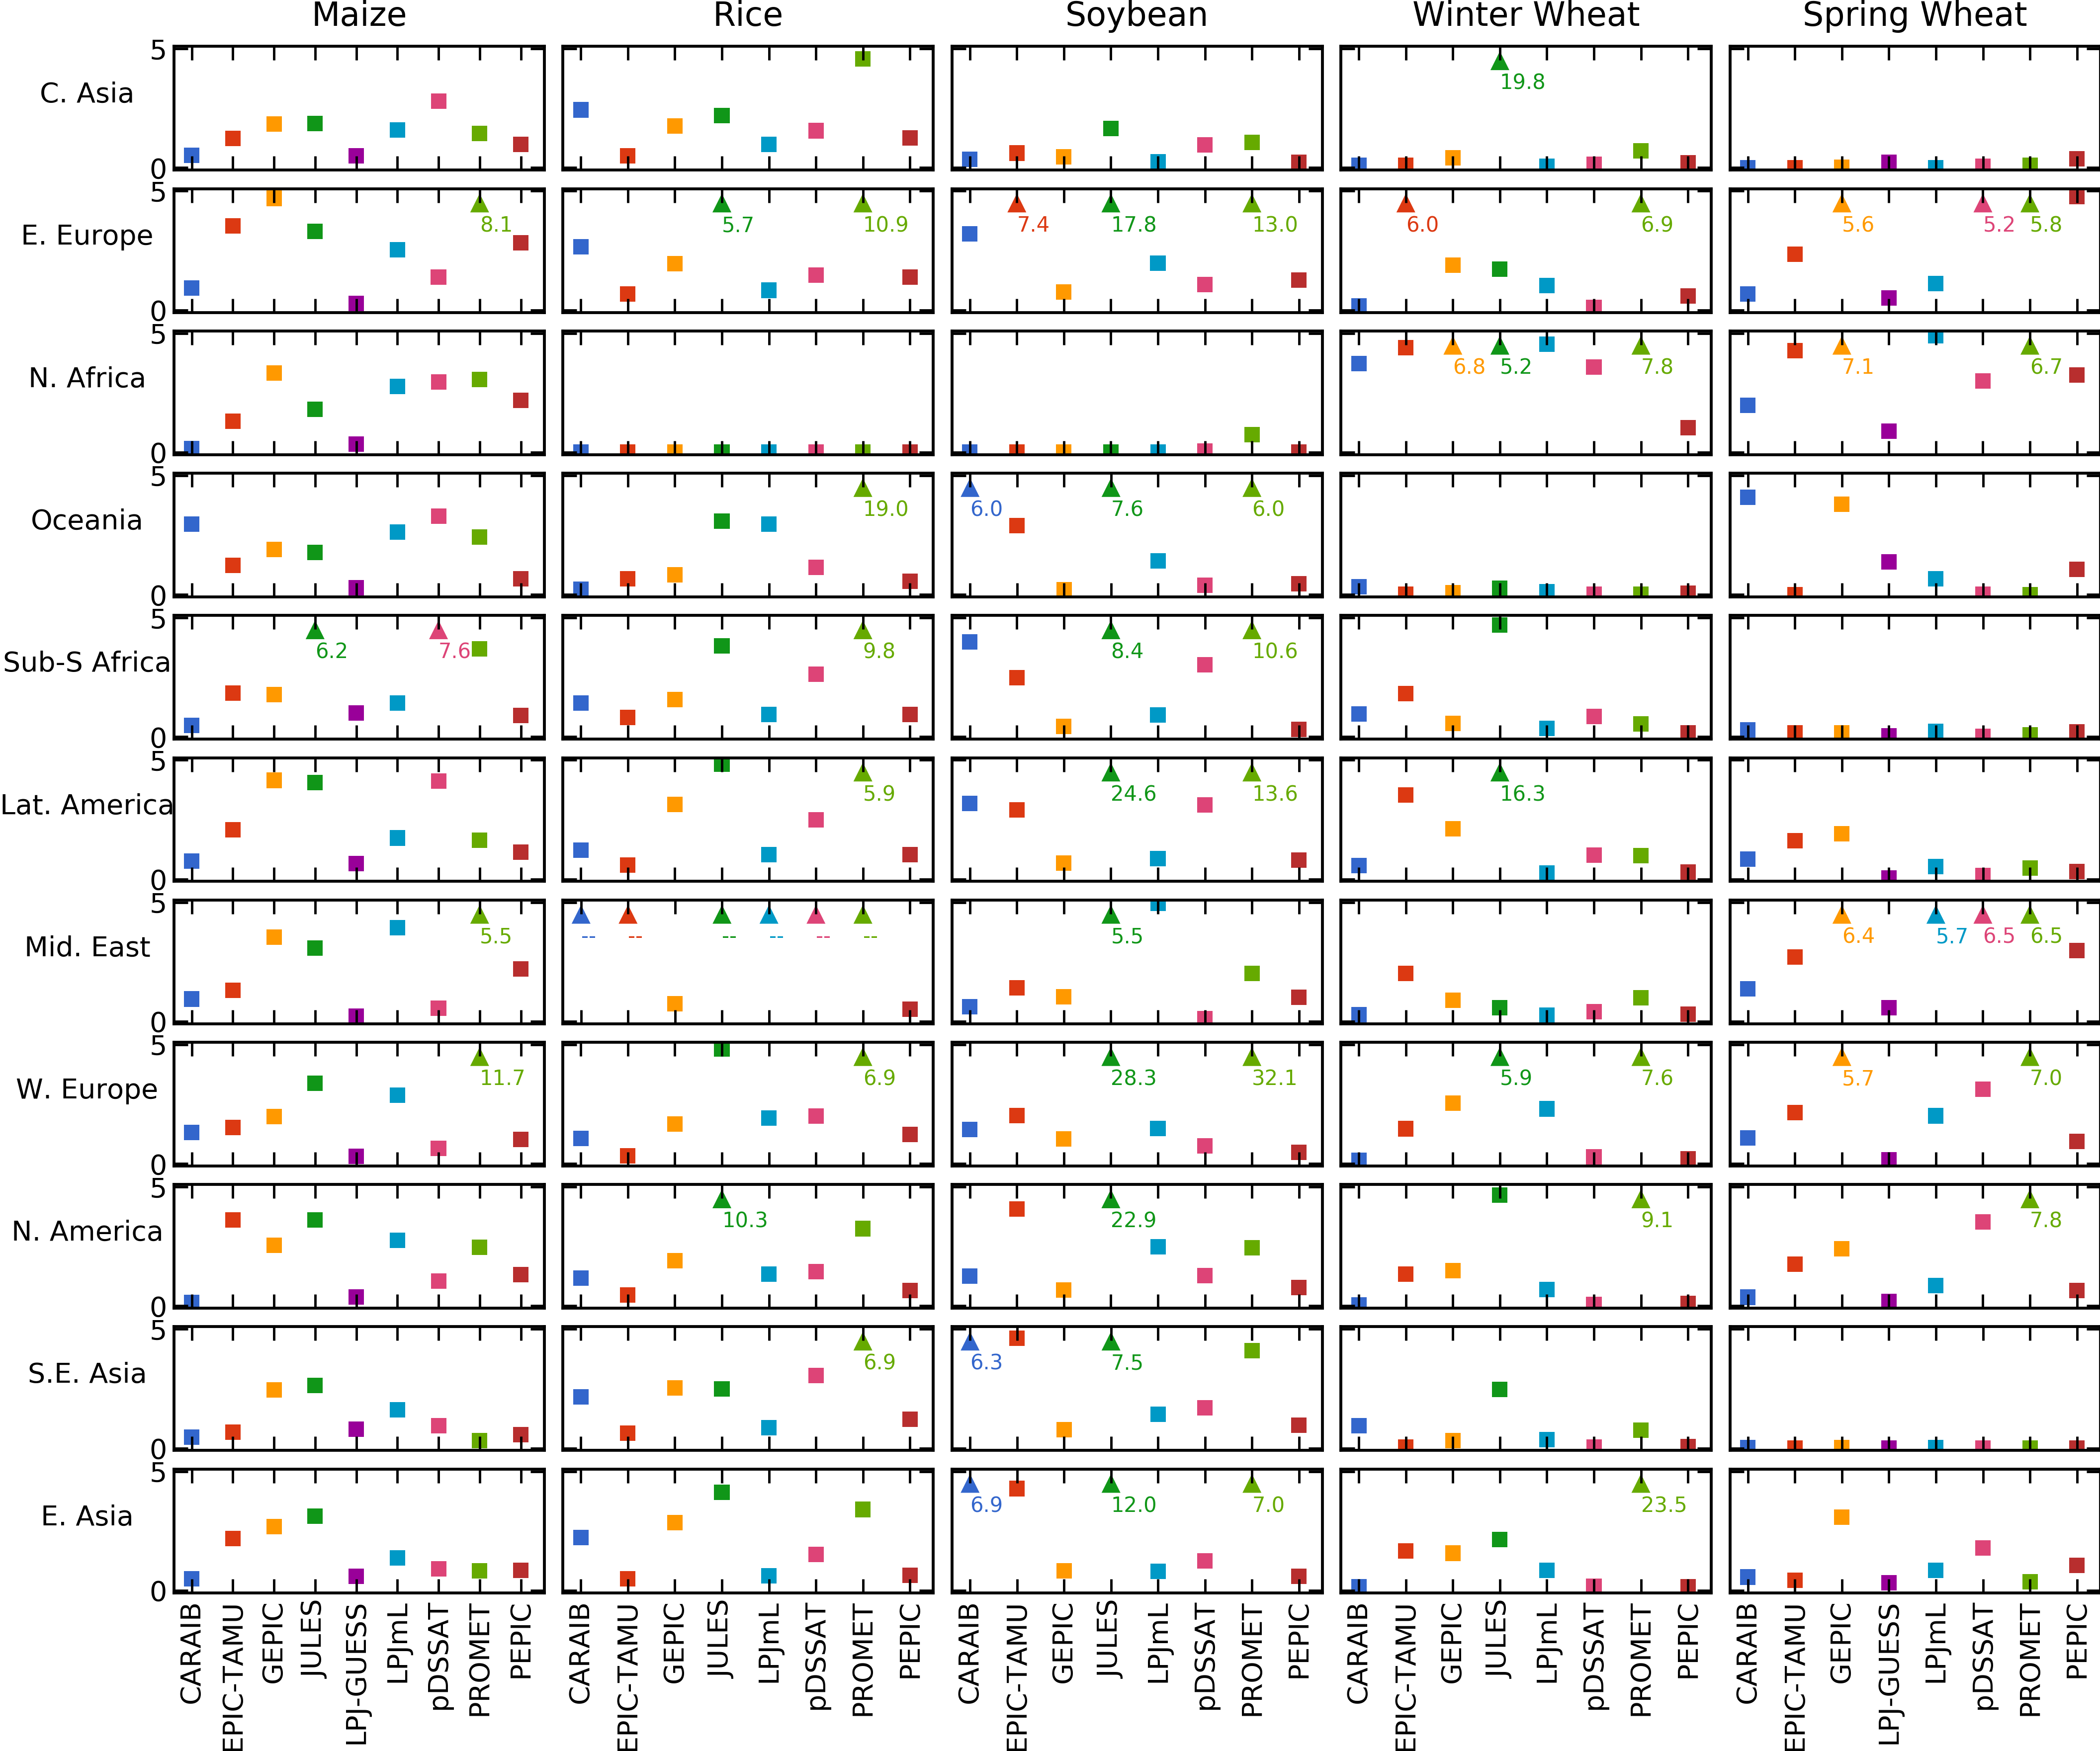
\includegraphics[width = 15cm]{figures/emulator_error.png}
  \caption{
    Mean absolute error of emulator representation of a simulation as a percentage of baseline simulated yield for the cross-validation process for rainfed crops. 
    A 4-fold stratified k-fold cross validation scheme is utilized where the model is trained on 75\% of the data and validated on the held-out 25\% (repeated four times). 
    The split does not represent a uniform number of samples in each location or in each model because simulation sampling extent in variable space is heterogeneous. 
    The table shows the mean error (as a percentage of baseline yield) weighted by hectares grown in each grid cell.
  }
  \label{fig:all_dims}
\end{figure*}


\Author[1,2]{James}{Franke}
\Author[3]{Christoph}{M\"{u}ller}
\Author[2,4]{Joshua}{Elliott}
\Author[5]{Alex C.}{Ruane}
\Author[6]{Abigail}{Snyder}
\Author[3,2,4,5]{Jonas}{J\"{a}germeyr}
%\Author[7,8]{Juraj}{Balkovic}
\Author[9,10]{Philippe}{Ciais}
\Author[11]{Marie}{Dury}
\Author[12]{Pete}{Falloon}
%\Author[7]{Christian}{Folberth}
\Author[11]{Louis}{Fran{\c{c}}ois}
\Author[13]{Tobias}{Hank}
%\Author[14,23]{Munir}{Hoffmann}
\Author[15,16]{R.\ Cesar}{Izaurralde}
\Author[11]{Ingrid}{Jacquemin}
\Author[15]{Curtis}{Jones}
%\Author[7]{Nikolay}{Khabarov}
\Author[14]{Marian}{Koch}
\Author[2,17]{Michelle}{Li}
\Author[9,18]{Wenfeng}{Liu}
\Author[19]{Stefan}{Olin}
\Author[5,20]{Meridel}{Phillips}
\Author[21,22]{Thomas A.\ M.}{Pugh}
\Author[15]{Ashwan}{Reddy}
%\Author[9,10]{Xuhui}{Wang}
\Author[12]{Karina}{Williams}
\Author[13]{Florian}{Zabel}
\Author[1,2]{Elisabeth}{Moyer}
%%%%%%%%%%%%%%%%%%%%%%%%%%%%%%
\affil[1]{Department of the Geophysical Sciences, University of Chicago, Chicago, IL, USA}
\affil[2]{Center for Robust Decision-making on Climate and Energy Policy (RDCEP), University of Chicago, Chicago, IL, USA}
\affil[3]{Potsdam Institute for Climate Impact Research, Member of the Leibniz Association, Potsdam, Germany}
\affil[3]{Department of Computer Science, University of Chicago, Chicago, IL, USA}
\affil[5]{NASA Goddard Institute for Space Studies, New York, NY, United States}
\affil[6]{Joint Global Change Research Institute, Pacific Northwest National Laboratory, College Park, MD, USA}
%\affil[7]{Ecosystem Services and Management Program, International Institute for Applied Systems Analysis, Laxenburg, Austria}
%\affil[8]{Department of Soil Science, Faculty of Natural Sciences, Comenius University in Bratislava, Bratislava, Slovak Republic}
\affil[9]{Laboratoire des Sciences du Climat et de l'Environnement, CEA-CNRS-UVSQ, 91191 Gif-sur-Yvette, France}
\affil[10]{Sino-French Institute of Earth System Sciences, College of Urban and Env. Sciences, Peking University, Beijing, China}
\affil[11]{Unit{\'{e}} de Mod{\'{e}}lisation du Climat et des Cycles Biog\'eochimiques, UR SPHERES, Institut d'Astrophysique et de G\'eophysique, University of Li\`ege, Belgium}
\affil[12]{Met Office Hadley Centre, Exeter, United Kingdom}
\affil[13]{Department of Geography, Ludwig-Maximilians-Universit\"{a}t, Munich, Germany}
\affil[14]{Georg-August-University G\"{o}ttingen, Tropical Plant Production and Agricultural Systems Modeling, G\"{o}ttingen, Germany}
\affil[15]{Department of Geographical Sciences, University of Maryland, College Park, MD, USA}
\affil[16]{Texas Agrilife Research and Extension, Texas A\&M University, Temple, TX, USA}
\affil[17]{Department of Statistics, University of Chicago, Chicago, IL, USA}
\affil[18]{EAWAG, Swiss Federal Institute of Aquatic Science and Technology, D\"{u}bendorf, Switzerland}
\affil[19]{Department of Physical Geography and Ecosystem Science, Lund University, Lund, Sweden}
\affil[20]{Earth Institute Center for Climate Systems Research, Columbia University, New York, NY, USA}
\affil[21]{School of Geography, Earth and Environmental Sciences, University of Birmingham, Birmingham, UK.}
\affil[22]{Birmingham Institute of Forest Research, University of Birmingham, Birmingham, UK.}
\affil[23]{Leibniz Centre for Agricultural Landscape Research (ZALF), D-15374 Müncheberg, Germany}


%\begin{figure*}[ht]
%\centering
   %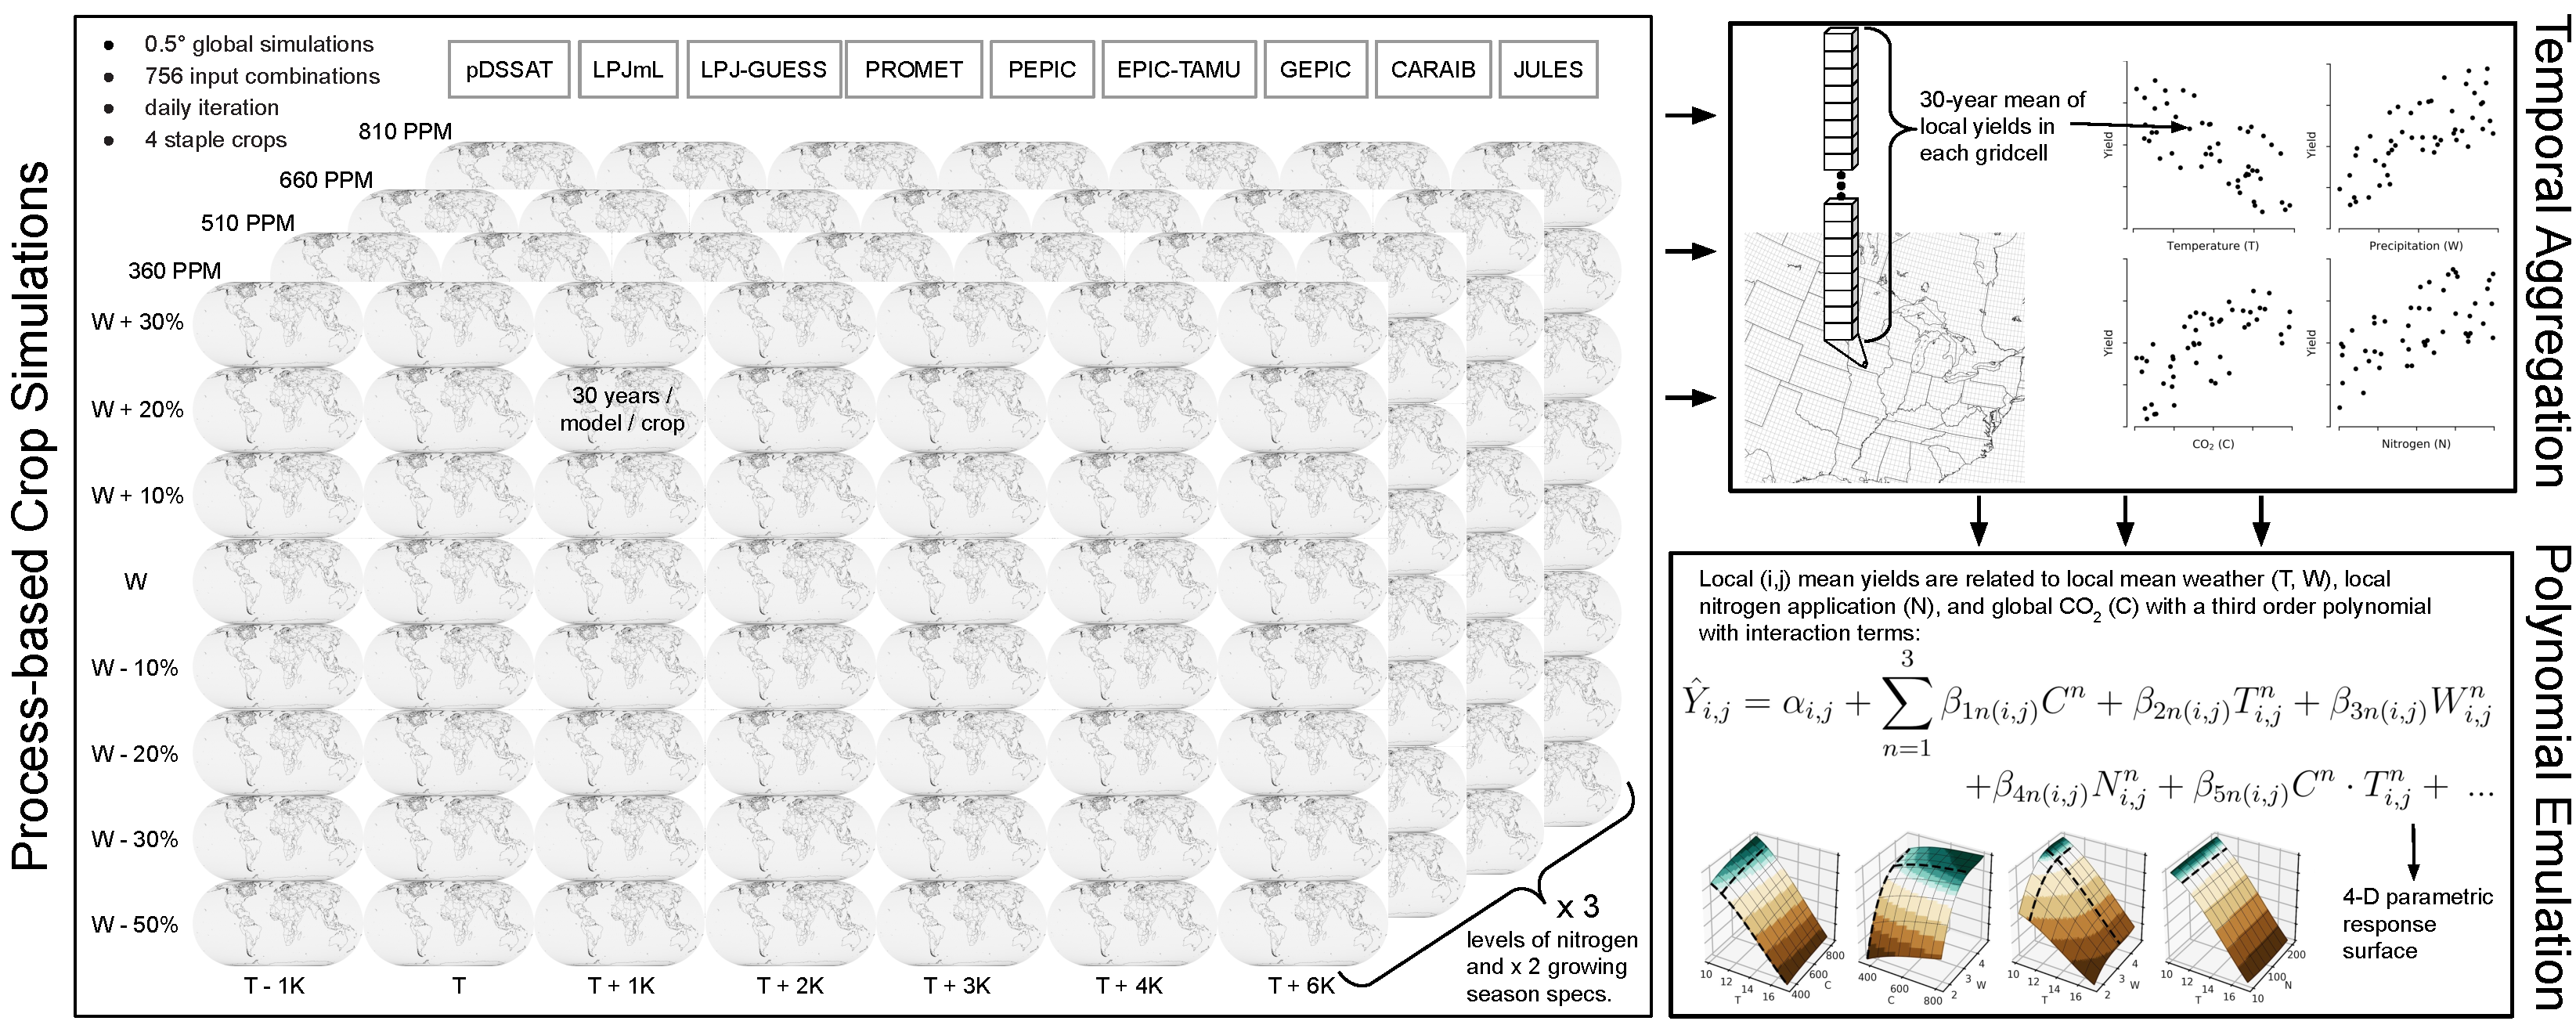
\includegraphics[width=17.5cm]{figures/flowchart.pdf}
   %%\caption{
   %Conceptual framework. 
   %}
   %\label{fig:yearvclim}
%\end{figure*}

%\textcolor{red}{The experiment involves twelve different globally gridded crop models, each simulating multiple crops (maize, rice, soybean and spring and winter wheat) over as many as 1400 simulations, each driven by historical climate inputs with systematically perturbations to CO$_2$, temperature, precipitation, and nitrogen application (CTWN).
%The resulting dataset allows }
%is the most comprehensive crop model emulation effort to date, significantly expanding the scope of previous parameter-sweep crop model emulation work by incorporating 

 %Furthermore, the year-over-year response is nonlinear with baseline climate: while the climatological response is nearly the same in T+0 to T+6 scenarios, evolving only from XX-XX tons ha$^{-1}$/K, the year-over-year response rises by over a quarter, from 1.9 to 2.5 tons ha$^{-1}$/K. 
%The same general principal applies to a lesser degree the precipitation dimension however in this case it is more manifestly an artifact of sampling range in the historical period (Figure \ref{fig:yearvclim}, right).

%While differences in year-over-year and climatological temperature responses can arise for many reasons, including memory in the crop model and lurking covariates, the most reasonable explanation is that the regressors here, mean growing-season temperature, does not fully describe the conditions that affect crop yields. That is, changes in growing-season temperature \textit{means}  may involve different changes in growing-season temperature \textit{distributions}  in the forced and unforced cases \citep[e.g.][]{Ruane2016}. 
%In the GGCMI Phase II experiment, the imposed perturbations involve no changes in underlying distributions (reasonable since summertime change are expected to be small \cite{XX}), but year-over-year variations are \textit{XX}. Note that year-over-year distributions of yields do become wider in highly impacted climate states in GGCMI Phase II (Figure \ref{fig:yearly}), but only because yield responses to both temperature and precipitation perturbations are nonlinear.
%It is expected that precipitation perturbations would produce more similar responses on year-over-year and climatological scales, because changes in precipitation distributions affect yields less than do those in temperature. Crops respond not to precipitation but to soil moisture, which integrates on timescales of weeks or even months \cite{XX}. Previous studies have suggested that in all but very arid regions, yields are not sensitive to how precipitation is distributed within a month \citep{Glotter14}.

%Ensemble spread dependence can be readily seen when comparing assessments of emulator performance in simulations at baseline CO$_2$ (Figure \ref{fig:error_360}) with those at higher CO$_2$ levels (Figure SXX) because models disagree on the magnitude of CO$_2$ fertilization. 
%We therefore do not provide a formal parameter uncertainty analysis, but note that the GGCMI Phase II dataset is well-suited to statistical exploration of emulation approaches and quantification of emulator fidelity. 
%More rigorous emulator assessments that could be preformed in future work include: testing other statistical specifications including non-parametric models and calculating standard error on emulator parameters.

%construct this test in some case we are extrapolating, which is not the intended use... 
%cross validation process often does not include ``edge'' simulations in the training set (i.e. those at the highest or lowest value in that dimension) on one or more folds of the training set split.
%The ``edge'' cases are then predicted during the prediction phase of cross validation.
%Such an extrapolation during cross validation is not representative based on the intended use of the emulator, which should only be used within the sample space of the overall training set.
%(the process is then repeated four times to cover all data in the training set). 
